\documentclass[11pt,aspectratio=169]{beamer}

% --- Tema og fonte ---
\usetheme{Madrid}
\usefonttheme{serif}
% --- Farver ---
\definecolor{myteal}{RGB}{14,71,57}
\setbeamercolor{title}{fg=white}
\setbeamercolor{frametitle}{fg=white,bg=myteal}
\setbeamercolor{block title}{fg=white,bg=myteal}
\setbeamercolor{block body}{bg=myteal!10}
\setbeamercolor{normal text}{fg=myteal}
\setbeamercolor{background canvas}{bg=white}
\setbeamercolor{structure}{fg=myteal}
\setbeamercolor{palette primary}{fg=white,bg=myteal}
\setbeamercolor{palette secondary}{fg=white,bg=myteal!80}
\setbeamercolor{palette tertiary}{fg=white,bg=myteal!60}
\setbeamercolor{author in head/foot}{fg=white,bg=myteal}
\setbeamercolor{title in head/foot}{fg=white,bg=myteal!80}
\setbeamercolor{date in head/foot}{fg=white,bg=myteal!60}
\setbeamercolor{titlelike}{fg=myteal}
\setbeamercolor{section in toc}{fg=myteal}
\setbeamercolor{item}{fg=myteal}
% --- Sprog og encoding ---
\usepackage[utf8]{inputenc}
\usepackage[danish]{babel}
\usepackage[T1]{fontenc}
\usepackage{lmodern}
% --- Matematik ---
\usepackage{amsmath,amsfonts,amssymb}
% --- Grafik og layout ---
\usepackage{graphicx}
\usepackage{ragged2e}
\usepackage{booktabs}
\usepackage{arydshln}
\usepackage[most]{tcolorbox}
% --- Ikoner og figurer ---
\usepackage{fontawesome5}
\usepackage{tikz}
\usetikzlibrary{positioning,arrows.meta,shapes.geometric,calc}
\usepackage{circuitikz}
% --- Positionering ---
\usepackage[absolute,overlay]{textpos}
% --- CSV ---
\usepackage{csvsimple}
% --- Kildehenvisning nederst på slides ---
\setbeamercolor{framesource}{fg=gray,bg=white}
\setbeamerfont{framesource}{size=\scriptsize}
\newcommand{\framesource}[1]{%
  \begin{textblock*}{12cm}(0.5cm,8.6cm)
    \raggedleft
    \beamercolorbox[wd=\textwidth,rightskip=0.5cm]{framesource}{#1}
  \end{textblock*}
}
% --- Automatisk billedattribution ---
\csvreader[
  head to column names,
  no head
]{Billeder/billedkilder.csv}{}{}
\newcommand{\billedkilde}[1]{%
  \csvreader[
    head to column names,
    full filter=\ifcsvstrcmp{\filnavn}{#1}{\csvfilteraccept}{\csvfilterreject},
    no head
  ]{Billeder/billedkilder.csv}{}%
  {%
    \tiny\forfatter\ / Wikimedia Commons (\licens)%
  }%
}
% --- Boksstile til jagttid-sliden ---
\tcbset{
  gruppe/.style={
    enhanced,
    colback=white,
    colframe=myteal,
    coltitle=myteal,
    boxrule=0.8pt,
    dashed,
    sharp corners,
    fonttitle=\bfseries\large,
    attach boxed title to top left={yshift=-2mm,xshift=3mm},
    boxed title style={colback=white,colframe=white,boxrule=0pt,sharp corners},
    top=1mm,left=1mm,right=1mm,bottom=1mm
  },
  felt/.style={
    enhanced,
    colback=white,
    colframe=myteal,
    boxrule=0.6pt,
    sharp corners,
    halign=center,
    valign=center,
    width=\linewidth,
    height=1.55cm,
    fit,
    fit algorithm=fontsize,
    fit basedim=7pt,
    boxsep=0.3mm,
    left=0.5mm, right=0.5mm, top=0.3mm, bottom=0.3mm
  },
  feltfri/.style={
    enhanced,
    colback=white,
    colframe=myteal,
    boxrule=0.6pt,
    sharp corners,
    halign=center,
    valign=center,
    width=\linewidth,
    boxsep=0.3mm,
    left=0.5mm, right=0.5mm, top=0.3mm, bottom=0.3mm,
    fontupper=\scriptsize
  }
}
% --- Matematiske operatorer ---
\DeclareMathOperator{\sen}{sen}
\DeclareMathOperator{\tg}{tg}
% --- Beamer-indstillinger ---
\setbeamertemplate{caption}[numbered]
\setbeamertemplate{navigation symbols}{}
% --- Forfatter ---
\author[Østerbro Jagttegn]{Østerbro Jagttegn \\ \textbf{Aleksander Sønder}}
% --- Hyperref (altid sidst) ---
\usepackage{hyperref}
\hypersetup{
  colorlinks=true,
  linkcolor=myteal,
  urlcolor=myteal,
  citecolor=myteal
}

\title{Obligatorisk Teori 2 \\ Hold ss26}
\date{\today}

\begin{document}

% Titelside
\begin{frame}
  \titlepage
\end{frame}

% Indholdsfortegnelse (valgfri)
\begin{frame}{Program}
  \tableofcontents
\end{frame}

\section{Artsfredningsbekendtgørelsen}

\begin{frame}
  \vspace{3em}
  \begin{center}
    {\LARGE \textbf{Artsfredningsbekendtgørelsen}}
    \vspace{2em}
    \\ Bekendtgørelse om fredning af visse dyre- og plantearter og pleje af tilskadekommet vildt
\par
% Våbenbekendtgørelsen
{\normalsize \href{https://www.retsinformation.dk/eli/lta/2021/521}{BEK nr 521 af 25/03/2021 \\ §§ 1-9 | § 10, stk. 1 | § 11 | §§ 25-31}}
\vspace{1em}
\par
  \end{center}
\end{frame}

\begin{frame}{Anvendelsesområde}
\begin{itemize}
  \item Bekendtgørelsen omfatter:
  \begin{itemize}
    \item Fuglearter i vild tilstand i EU-Europa (fuglebeskyttelsesdirektivet)
    \item Pattedyr, krybdyr, fisk, padder, invertebrater (bilag 1)
    \item Planter (bilag 2)
    \item Dyr fra bilag 3 (igler/snegle mv.)
  \end{itemize}
  \item Gælder også udsatte/undslupne pattedyr \& fugle med vildtlevende, reproducerende bestande (ikke traditionelle husdyr)
  \item Omfatter alle livsstadier + dele/produkter (dyr \& planter)
  \item Vildt = naturligt forekommende pattedyr \& fugle i DK (inkl. trækfugle)
\end{itemize}
\end{frame}

\begin{frame}{Undtagelser}
\begin{itemize}
  \item \textbf{Gælder ikke:}
  \begin{itemize}
    \item Landbrugsmæssigt opdrættede dyr (jf. lov om hold af dyr)
    \item Dyr opdrættet i fangenskab af lovligt erhvervede forældre
  \end{itemize}
  \end{itemize}
\end{frame}

\begin{frame}{Forbud mod drab \& indfangning}
\begin{itemize}
  \item Forsætligt drab eller indfangning af vilde fugle (§ 1, stk. 1) forbudt – uanset metode
  \item Også forbud mod besiddelse af levende vilde fugle
  \item Gælder IKKE for arter der må
  \begin{itemize}
    \item jages/indfanges efter jagttidsbekendtgørelsen
    \item reguleres efter vildtskadebekendtgørelsen
  \end{itemize}
\end{itemize}
\end{frame}

\begin{frame}{Forbud mod handel mv.}
\begin{itemize}
  \item Forbud mod handel, transport til handel, opbevaring til handel, udbud til salg, konservering, udstilling af vilde fugle (§ 1, stk. 1 \& 3)
  \item Gælder også genkendelige dele \& produkter
  \item \textbf{Undtagelse:} Gælder IKKE for fugle på \textbf{bilag 4}, hvis lovligt dræbt/indfanget/erhvervet
\end{itemize}
\end{frame}

\begin{frame}{Bilag 4 – Arter der kan handles (undtagelse fra forbud)}
\tiny
Fugle fra fuglebeskyttelsesdirektivets bilag III A/B – handel tilladt hvis lovligt erhvervet.\\
* = Invasive (EU 1143/2014: forbud mod handel med levende eksemplarer)

\begin{itemize}
  \item Agerhøne \textit{(Perdix perdix)}
  \item Amerikansk skarveand \textit{(Oxyura jamaicensis)} *
  \item Canadagås \textit{(Branta canadensis)}
  \item Fasan \textit{(Phasianus colchicus)}
  \item Grågås \textit{(Anser anser)}
  \item Gråand \textit{(Anas platyrhynchos)}
  \item Krikand \textit{(Anas crecca)}
  \item Nilgås \textit{(Alopochen aegyptiaca)} *
  \item Ringdue \textit{(Columba palumbus)}
  \item Skovsneppe \textit{(Scolopax rusticola)}
\end{itemize}

\tiny
Undtagelse: Tillader handel, transport, opbevaring, konservering, udstilling mv.
\end{frame}

\begin{frame}{Beskyttelse af redetræer \& reder}
\begin{itemize}
  \item Kolonirugende fugles redetræer: fædningsforbud 1. feb.–31. jul.
  \item Rovfugle \& uglers redetræer: fældningsforbud 1. feb.–31. aug.
  \item Ørne, sort stork, rød glente: redetræer må \textbf{aldrig} fældes
  \item Hule træer \& træer med spættehuller: fældningsforbud 1. nov.–31. aug.
  \item Digesvalereder: må ikke ødelægges 1. apr.–31. aug.
\end{itemize}
\end{frame}

\begin{frame}{Import \& handel med levende fugle}
\begin{itemize}
  \item Forbud mod import af levende fugle (fuglebeskyttelsesdirektivet, artikel 1) fra lande uden for EU – medmindre dokumenteret fangenskabsopdræt
  \item Gælder også underarter (selvom ikke naturlige i EU)
  \item Handel/forsendelse af levende fugle: kun tilladt hvis fangenskabsopdrættet er registreret
  \item Dokumentationspligt over for Miljøstyrelsen
\end{itemize}
\end{frame}

\begin{frame}{Streng beskyttelse (Habitatdirektiv bilag IV)}
\begin{itemize}
  \item Gælder vildtlevende dyr på habitatdirektivets bilag IV (jf. bilag 1 i bekendtgørelsen)
  \item \textbf{Totalt forbud} mod:
  \begin{itemize}
    \item Alle former for forsætlig indfangning eller drab
    \item Forsætlig ødelæggelse/ind samling af æg i naturen
  \end{itemize}
  \item Planter på bilag IV (jf. bilag 2): Forbud mod forsætlig plukning, indsamling, afskæring, opgravning, oprivning med rod eller ødelæggelse
  \item Eksempler: Mange flagermus, odder, ulv (tidl.), visse padder/insekter, orkideer mv.
  \item \textbf{Hovedregel:} Ingen undtagelse for jagt – strengeste niveau!
\end{itemize}
\end{frame}


\begin{frame}{Handel med jagtbart vildt}
\begin{itemize}
  \item
  \begin{itemize}
    \item Handel/transport af \textbf{døde pattedyr} tilladt – hvis lovligt nedlagt/ombragt
    \item \textbf{Levende vildt:} Kun efter tilladelse fra Miljøstyrelsen
  \end{itemize}
  \item Erhvervsmæssige købere skal dokumentere køb de sidste 2 år (hvad \& fra hvem) på Miljøstyrelsens forlangende
  \item \textbf{Budskab:} Sporbarhed er vigtig – ulovligt vildt må ikke handles
\end{itemize}
\end{frame}

\begin{frame}{Bilag 5 – Forbud mod konservering (dansk natur)}
\tiny
Pattedyr og fugle – ingen udstopning/konservering uden dispensation

\begin{columns}[T]
\column{0.33\textwidth}
\textbf{Pattedyr}
\begin{itemize}
  \item Birkemus (\textit{Sicista betulina})
  \item Hasselmus (\textit{Muscardinus avellanarius})
  \item Hvaler (Cetacea, alle)
  \item Odder (\textit{Lutra lutra})
  \item Småflagermus (Microchiroptera spp.)
  \item Ulv (\textit{Canis lupus})
  \item Bæver (\textit{Castor fiber})
\end{itemize}

\column{0.33\textwidth}
\textbf{Rovfugle \& ugler}
\begin{itemize}
  \item Blå kærhøg (\textit{Circus cyaneus})
  \item Dværgfalk (\textit{Falco columbarius})
  \item Fiskeørn (\textit{Pandion haliaetus})
  \item Havørn (\textit{Haliaeetus albicilla})
  \item Hedehøg (\textit{Circus pygargus})
  \item Jagtfalk (\textit{Falco rusticolus})
  \item Kongeørn (\textit{Aquila chrysaetos})
  \item Kirkeugle (\textit{Athene noctua})
  \item Mosehornugle (\textit{Asio flammeus})
  \item Lærkefalk (\textit{Falco subbuteo})
  \item Rød glente (\textit{Milvus milvus})
  \item Stor hornugle (\textit{Bubo bubo})
  \item Slangeørn (\textit{Circaetus gallicus})
  \item Vandrefalk (\textit{Falco peregrinus})
\end{itemize}

\column{0.33\textwidth}
\textbf{Andre fugle}
\begin{itemize}
  \item Biæder (\textit{Merops apiaster})
  \item Ellekrage (\textit{Coracias garrulus})
  \item Dværgterne (\textit{Sterna albifrons})
  \item Hvid stork (\textit{Ciconia ciconia})
  \item Hærfugl (\textit{Upupa epops})
  \item Høgesanger (\textit{Sylvia nisoria})
  \item Rørdrum (\textit{Botaurus stellaris})
  \item Sandterne (\textit{Gelochelidon nilotica})
  \item Sortterne (\textit{Chlidonias niger})
  \item Skestork (\textit{Platalea leucorodia})
  \item Sort stork (\textit{Ciconia nigra})
  \item Tinksmed (\textit{Tringa glareola})
  \item Trane (\textit{Grus grus})
  \item Pirol (\textit{Oriolus oriolus})
\end{itemize}
\end{columns}
\tiny
Gælder kun dyr fra dansk natur. Dispensation mulig (typisk kun museer mv.).
\end{frame}

\begin{frame}{Pleje af almindeligt tilskadekommet vildt udført af privat}
\begin{itemize}
  \item Gælder \textbf{ikke} vildtarter anført i bilag 6
  \item Må plejes med henblik på genudsætning (uanset fredningsregler i kap. 2-4)
  \item Genudsæt hurtigst muligt – helst på oprindeligt levested
  \item Hvis ingen realistisk genudsætning inden \textbf{6 måneder} → afliv hurtigst muligt
  \item Miljøstyrelsen kan dispensere i særlige tilfælde (på vilkår)
  \item \textbf{Budskab:} Hjælp OK, men begrænset tid – ingen permanent hold
\end{itemize}
\end{frame}

\begin{frame}{Pleje af strengt beskyttede arter (bilag 6) - kun særligt bemyndigede}
\begin{itemize}
  \item 
  \begin{itemize}
    \item Bilag 6-arter (fx odder, visse flagermus, ulv, bæver, sjældne fugle): Kun pleje hos \textbf{bemyndigede} personer/virksomheder 
    \item Ikke-omgående aflivning → kun hos bemyndiget
  \end{itemize}
  \item Miljøstyrelsen kan tilbagekalde bemyndigelse ved overtrædelser eller ved manglende formål
  \item \textbf{Budskab:} Streng kontrol – almindelige jagttegnsindehaver må ikke pleje disse arter
\end{itemize}
\end{frame}

\begin{frame}{Bilag 6 – Arter der kun må plejes af bemyndiget person/virksomhed}
\tiny
Tilskadekommet vildt eller nødstedt yngel (§ 30, stk. 3) – må IKKE plejes af private uden bemyndigelse fra Miljøstyrelsen/Styrelsen for Grøn Arealomlægning og Vandmiljø

\begin{columns}[T]
\column{0.5\textwidth}
\textbf{Pattedyr}
\begin{itemize}
  \item Bæver (\textit{Castor fiber})
  \item Flagermus (\textit{Chiroptera spp.}), alle arter
  \item Guldsjakal (\textit{Canis aureus})
  \item Hvaler (\textit{Cetacea spp.}), alle arter
  \item Kalve af krondyr, dådyr, sika (\textit{Cervus/Dama spp.})
  \item Lam af rådyr (\textit{Capreolus capreolus})
  \item Odder (\textit{Lutra lutra})
  \item Pindsvin (\textit{Erinaceus europaeus})
  \item Sæler (\textit{Phocidae spp.}), alle arter
  \item Ulv (\textit{Canis lupus})
\end{itemize}

\column{0.5\textwidth}
\textbf{Fugle}
\begin{itemize}
  \item Biæder (\textit{Merops apiaster})
  \item Ellekrage (\textit{Coracias garrulus})
  \item Engsnarre (\textit{Crex crex})
  \item Hærfugl (\textit{Upupa epops})
  \item Høgesanger (\textit{Curruca nisoria})
  \item Hvid stork (\textit{Ciconia ciconia})
  \item Hvidbrystet præstekrave (\textit{Charadrius alexandrinus})
  \item Isfugl (\textit{Alcedo atthis})
  \item Rørdrum (\textit{Botaurus stellaris})
  \item Rovfugle (\textit{Accipitriformes spp.}), alle arter
  \item Rovterne (\textit{Sterna caspia})
  \item Sandterne (\textit{Sterna nilotica})
  \item Sort stork (\textit{Ciconia nigra})
  \item Sortterne (\textit{Chlidonias niger})
  \item Trane (\textit{Grus grus})
  \item Ugler (\textit{Strigiformes spp.}), alle arter
\end{itemize}
\end{columns}

\tiny
Andre arter (ikke på bilag 6): Må plejes af alle med henblik på genudsætning (§ 29). Kontakt Styrelsen for Grøn Arealomlægning og Vandmiljø ved tvivl.
\end{frame}



\section{Dykænder}

\begin{frame}
  \vspace{3em}
  \begin{center}
    {\LARGE \textbf{Dykænder}}
    \vspace{2em}
    \\ Artsbestemmelse og vildtbiologi
\par
{\normalsize }
\vspace{1em}
\par
  \end{center}
\end{frame}

% ========== EDERFUGL ==========
\begin{frame}{%
  \begin{minipage}[c]{0.30\textwidth}
    Ederfugl
  \end{minipage}%
  \hfill
  \begin{minipage}[c]{0.45\textwidth}
    \footnotesize
    \textbf{Jagttid:} 1.\ oktober -- 31.\ januar \\[0.15em]
    {\scriptsize (kun hanner; hunner fredet)}
  \end{minipage}%
  \hfill
  \begin{minipage}[c]{0.15\textwidth}
    \noindent\raggedleft
    
\includegraphics[width=0.5cm, height=0.5cm, keepaspectratio]{Billeder/Ikoner/star.png}%
    \hspace{0.2em}%
    
\includegraphics[width=0.5cm, height=0.5cm, keepaspectratio]{Billeder/Ikoner/star.png}%
    \hspace{0.2em}%
    
\includegraphics[width=0.5cm, height=0.5cm, keepaspectratio]{Billeder/Ikoner/star.png}
  \end{minipage}%
}
  \vspace{0.25em}
  \begin{columns}[T]
    % --- Venstre kolonne: Tekst ---
    \column{0.55\textwidth}
    \setlength{\parskip}{0.5em}
    \tiny
    \RaggedRight
    \textbf{\textit{Somateria mollissima}} – største dykand i Danmark \par
    \textbf{Udseende:} \\
    \quad – Kok: Trekantet hoved, grønne aftegning i nakken, bølgeformede striber \par
    \quad – Høne: trekantet hoved, bølgeformede striber \par
    \textbf{Levesteder:} Kystfugl, på havet og i fjorde. \par
    \textbf{Føde:} Primært blåsmuslinger. \par
    \textbf{Udbredelse:} Både stationære og trækfugle. \par
    \textbf{Træk/standfugl:} Begge
    \begin{itemize}
      \itemsep0pt
      \item \textbf{Yngleforhold:} Yngler i hele Danmark.
      \item \textbf{Kønsmoden:} Ca. 3 år
      \item \textbf{Mono/polygam:} Monogam
      \item \textbf{Bestandsomsætning:} Langsom
      \item \textbf{Kuld:} 4–6 æg
      \item \textbf{Jagttid:} 1.\ oktober -- 31.\ januar (kun hanner; hunner fredet)
    \end{itemize}
    % --- Højre kolonne: To billeder ---
    \column{0.40\textwidth}
    \centering
    \fbox{%
      \begin{minipage}{\linewidth}
        \centering
        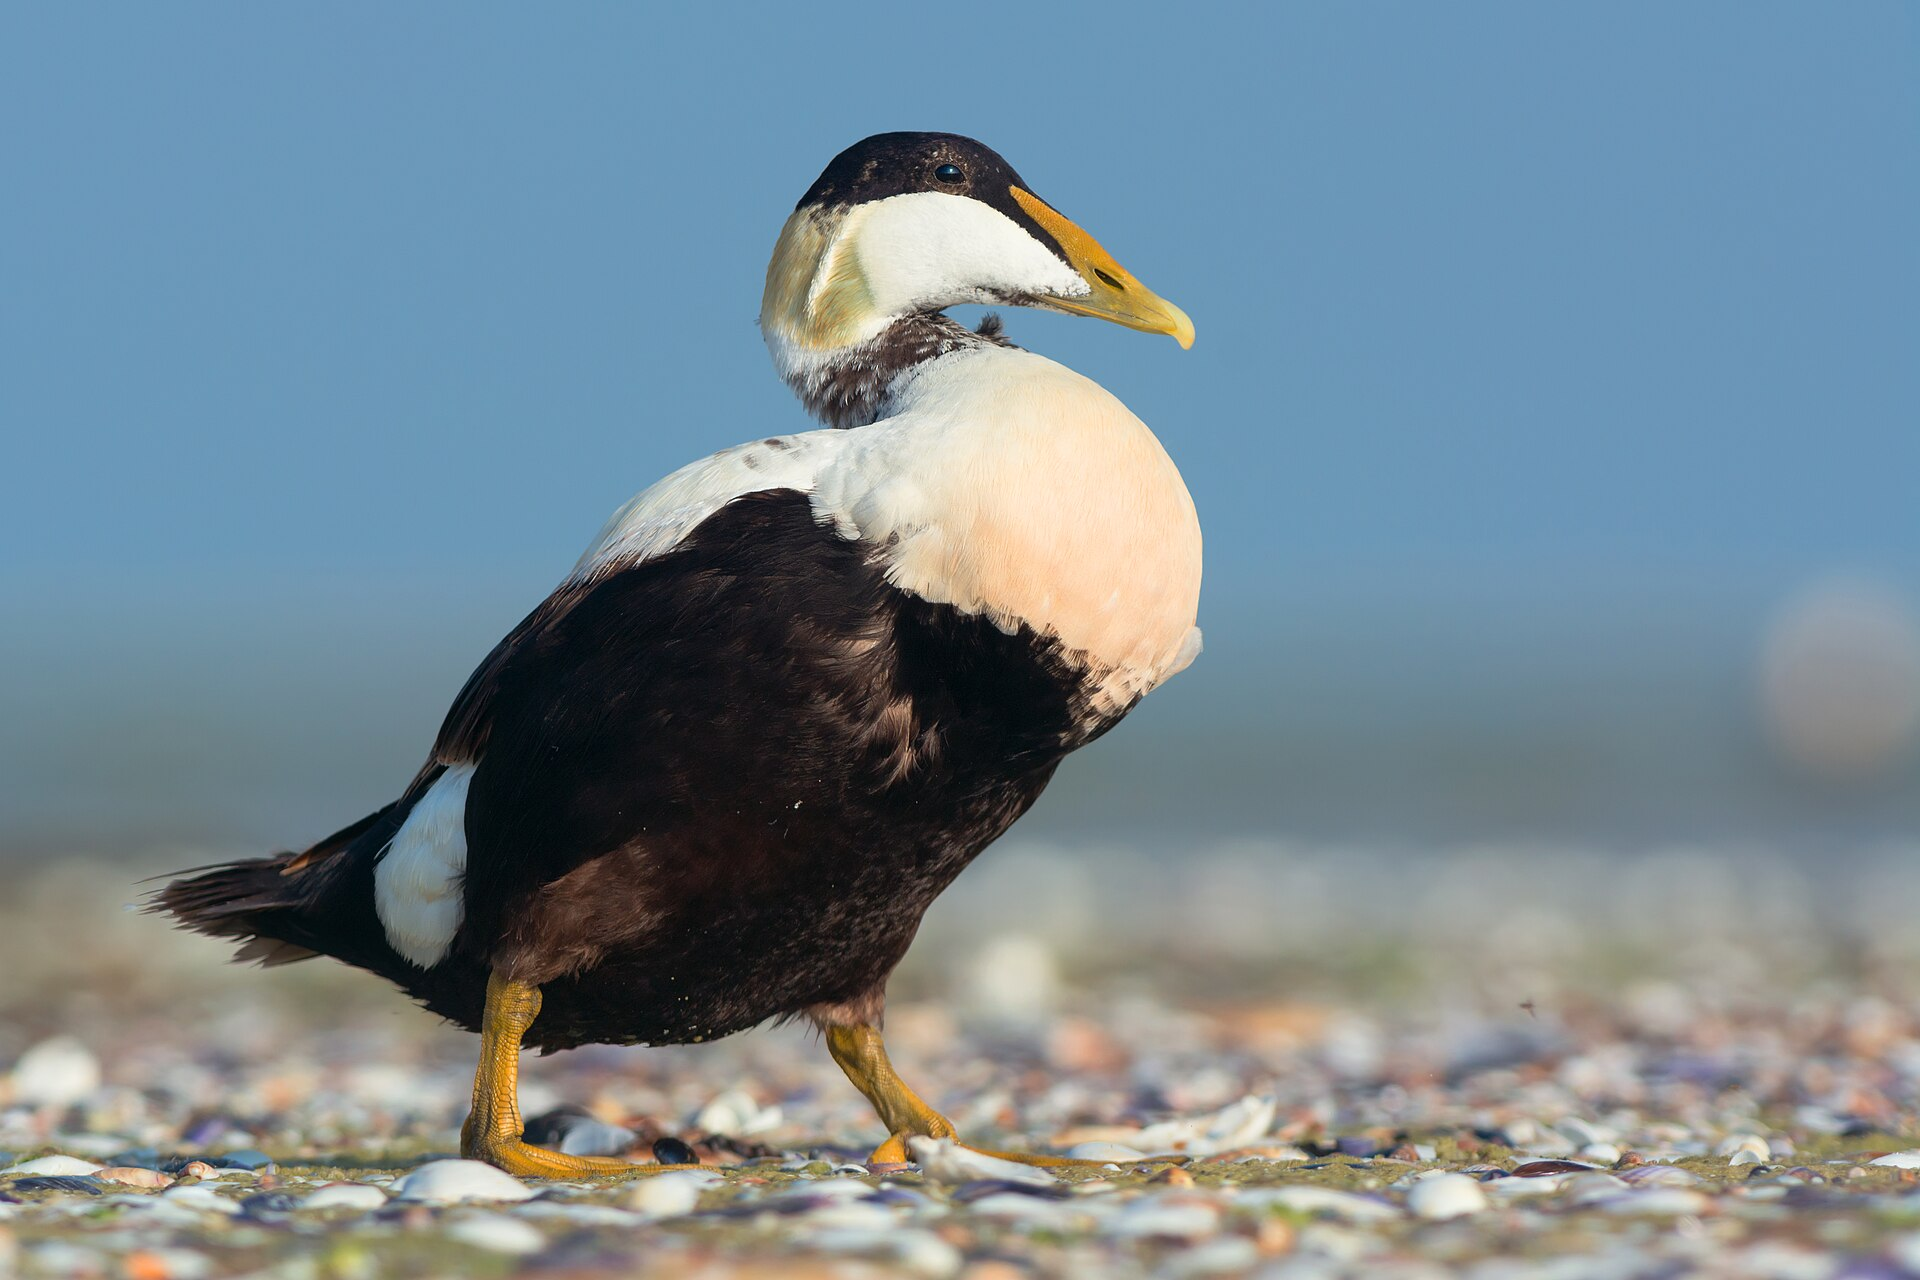
\includegraphics[width=0.7\linewidth, height=3cm, keepaspectratio]{Billeder/Dyr/Fugle/Aender/Dykaender/ederfugl_han.jpg}\\[0.5em]
        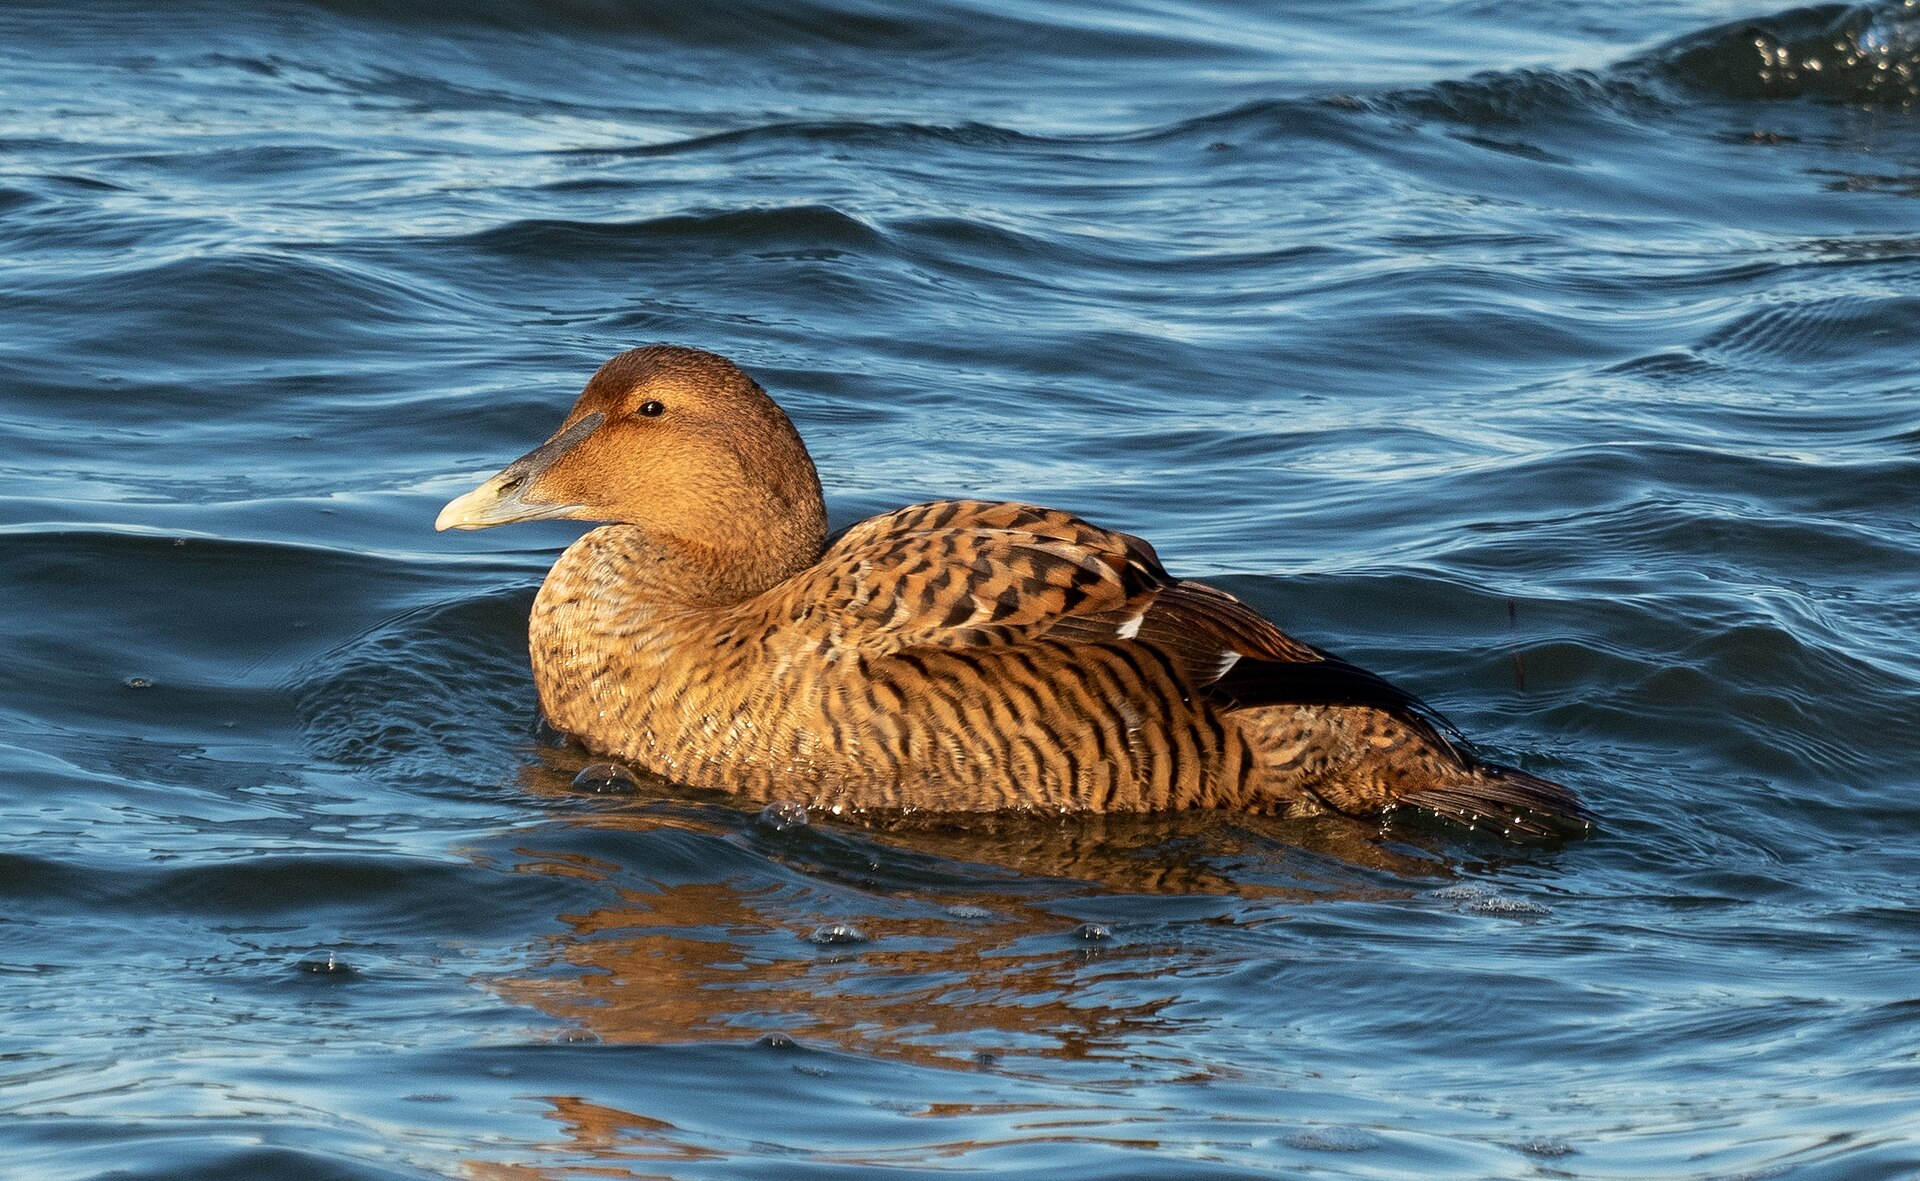
\includegraphics[width=0.7\linewidth, height=3cm, keepaspectratio]{Billeder/Dyr/Fugle/Aender/Dykaender/ederfugl_hun.jpg}
      \end{minipage}
    }%
    \vspace{0.05em}
    \footnotesize Han (kok) øverst, hun (høne) nederst
  \end{columns}
\end{frame}

% ========== HVINAND ==========
\begin{frame}{%
  \begin{minipage}[c]{0.30\textwidth}
    Hvinand
  \end{minipage}%
  \hfill
  \begin{minipage}[c]{0.45\textwidth}
    \footnotesize
    \textbf{Jagttid:} 1.\ oktober -- 31.\ januar
  \end{minipage}%
  \hfill
  \begin{minipage}[c]{0.15\textwidth}
    \noindent\raggedleft
    
\includegraphics[width=0.5cm, height=0.5cm, keepaspectratio]{Billeder/Ikoner/star.png}%
    \hspace{0.2em}%
    
\includegraphics[width=0.5cm, height=0.5cm, keepaspectratio]{Billeder/Ikoner/star.png}
  \end{minipage}%
}
  \vspace{0.25em}
  \begin{columns}[T]
    % --- Venstre kolonne: Tekst ---
    \column{0.55\textwidth}
    \setlength{\parskip}{0.5em}
    \tiny
    \RaggedRight
    \textbf{\textit{Bucephala clangula}} – mellemstor kraftig dykand \par
    \textbf{Udseende:}\\
    \quad – Andrik: Hvid plet på kinden \par
    \quad – And: Brunt hoved og askegrå krop \par
    \textbf{Levesteder:} Lavvandede kyster og beskyttede fjorde/vige. \par
    \textbf{Føde:} Snegle, muslinger, krebsdyr. \par
    \textbf{Udbredelse:} Hele Danmark. \par
    \textbf{Træk/standfugl:} Begge
    % --- Højre kolonne: Billeder ---
    \column{0.40\textwidth}
    \centering
    \fbox{%
      \begin{minipage}{\linewidth}
        \centering
        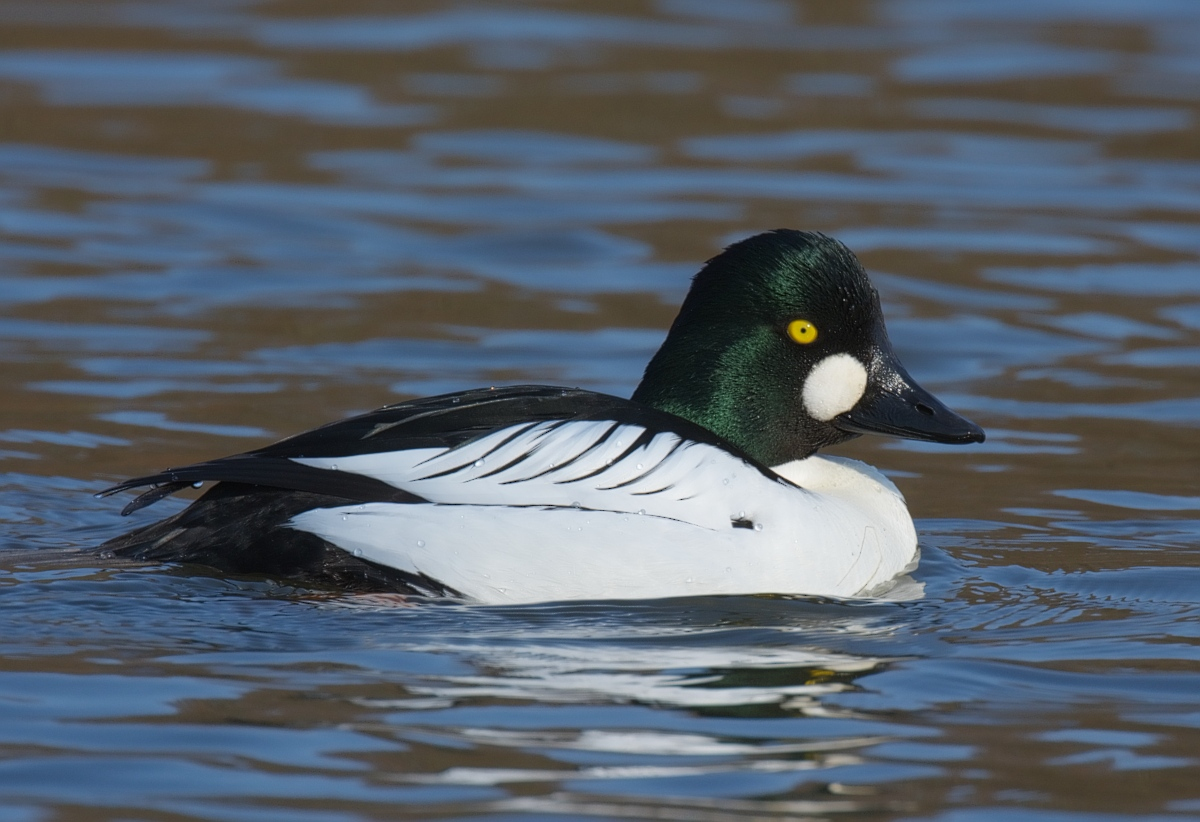
\includegraphics[width=0.7\linewidth, height=3cm, keepaspectratio]{Billeder/Dyr/Fugle/Aender/Dykaender/hvinand_han.jpg}\\[0.5em]
        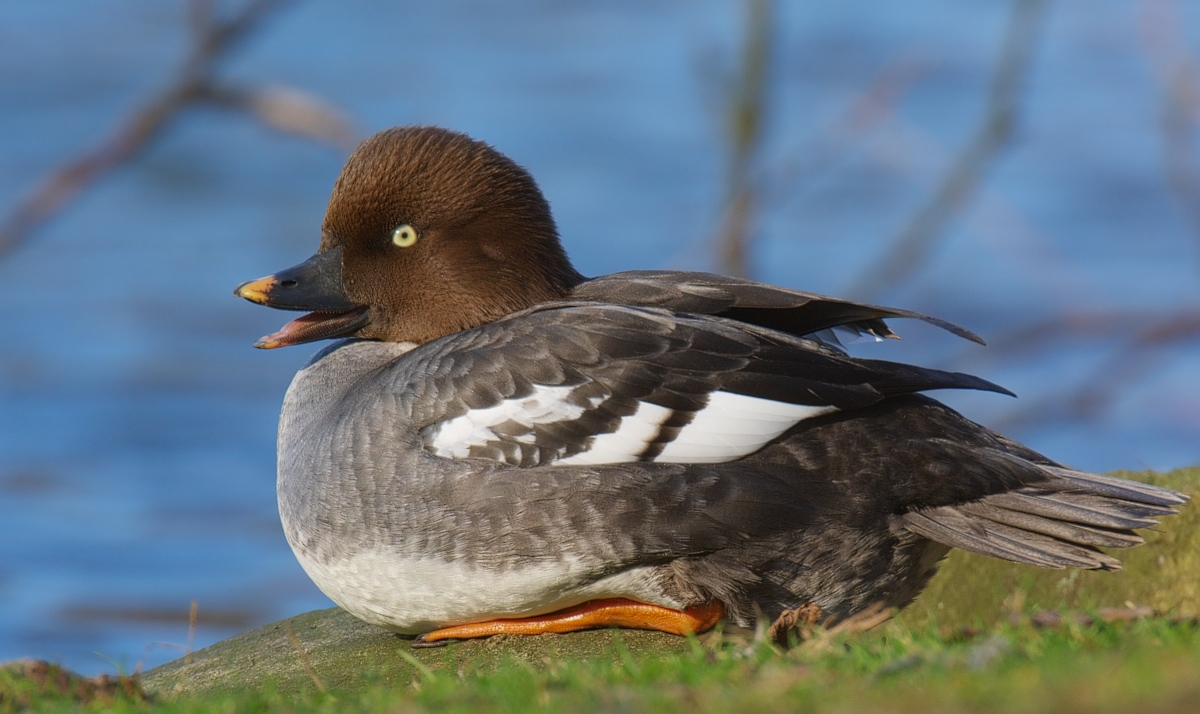
\includegraphics[width=0.7\linewidth, height=3cm, keepaspectratio]{Billeder/Dyr/Fugle/Aender/Dykaender/hvinand_hun.jpg}
      \end{minipage}
    }%
    \vspace{0.05em}
    \footnotesize Andrik øverst, and nederst
  \end{columns}
\end{frame}

% ========== TROLDAND ==========
\begin{frame}{%
  \begin{minipage}[c]{0.30\textwidth}
    Troldand
  \end{minipage}%
  \hfill
  \begin{minipage}[c]{0.45\textwidth}
    \footnotesize
    \textbf{Jagttid:} 1.\ oktober -- 31.\ januar
  \end{minipage}%
  \hfill
  \begin{minipage}[c]{0.15\textwidth}
    \noindent\raggedleft
    
\includegraphics[width=0.5cm, height=0.5cm, keepaspectratio]{Billeder/Ikoner/star.png}%
    \hspace{0.2em}%
    
\includegraphics[width=0.5cm, height=0.5cm, keepaspectratio]{Billeder/Ikoner/star.png}
  \end{minipage}%
}
  \vspace{0.25em}
  \begin{columns}[T]
    % --- Venstre kolonne: Tekst ---
    \column{0.55\textwidth}
    \setlength{\parskip}{0.5em}
    \tiny
    \RaggedRight
    \textbf{\textit{Aythya fuligula}} – lille dykand med karakteristisk nakketop \par
    \textbf{Udseende:}\\
    \quad – Andrik: Lang sort nakketop \par
    \quad – And: Lille sort nakketop \par
    \textbf{Levesteder:} Lavvandede vådområder og indre farvande. \par
    \textbf{Føde:} Muslinger, snegle og krebsdyr. \par
    \textbf{Udbredelse:} Hele Danmark. \par
    \textbf{Træk/standfugl:} Begge
    % --- Højre kolonne: Billeder ---
    \column{0.40\textwidth}
    \centering
    \fbox{%
      \begin{minipage}{\linewidth}
        \centering
        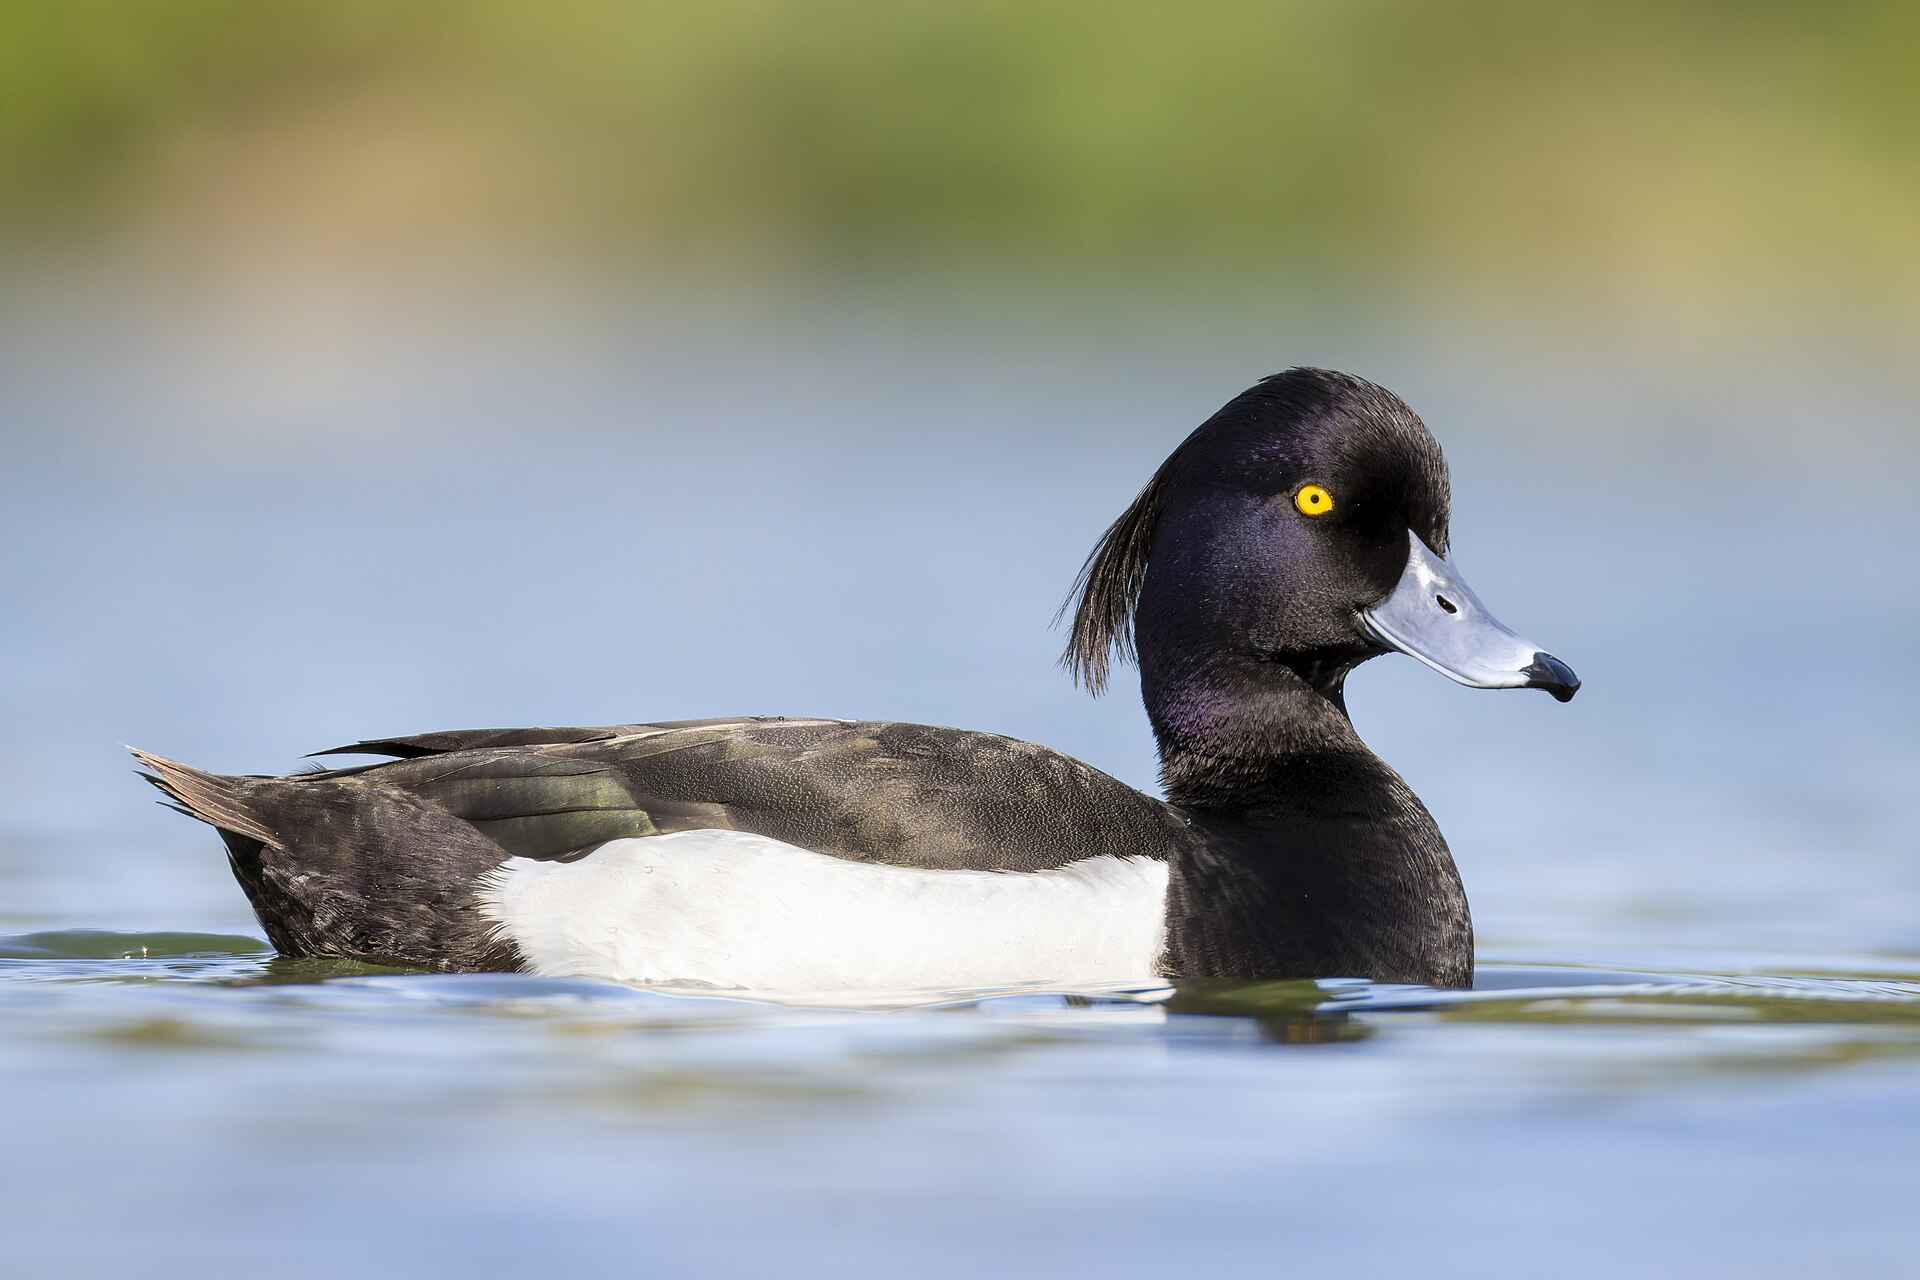
\includegraphics[width=0.7\linewidth, height=3cm, keepaspectratio]{Billeder/Dyr/Fugle/Aender/Dykaender/troldand_han.jpg}\\[0.5em]
        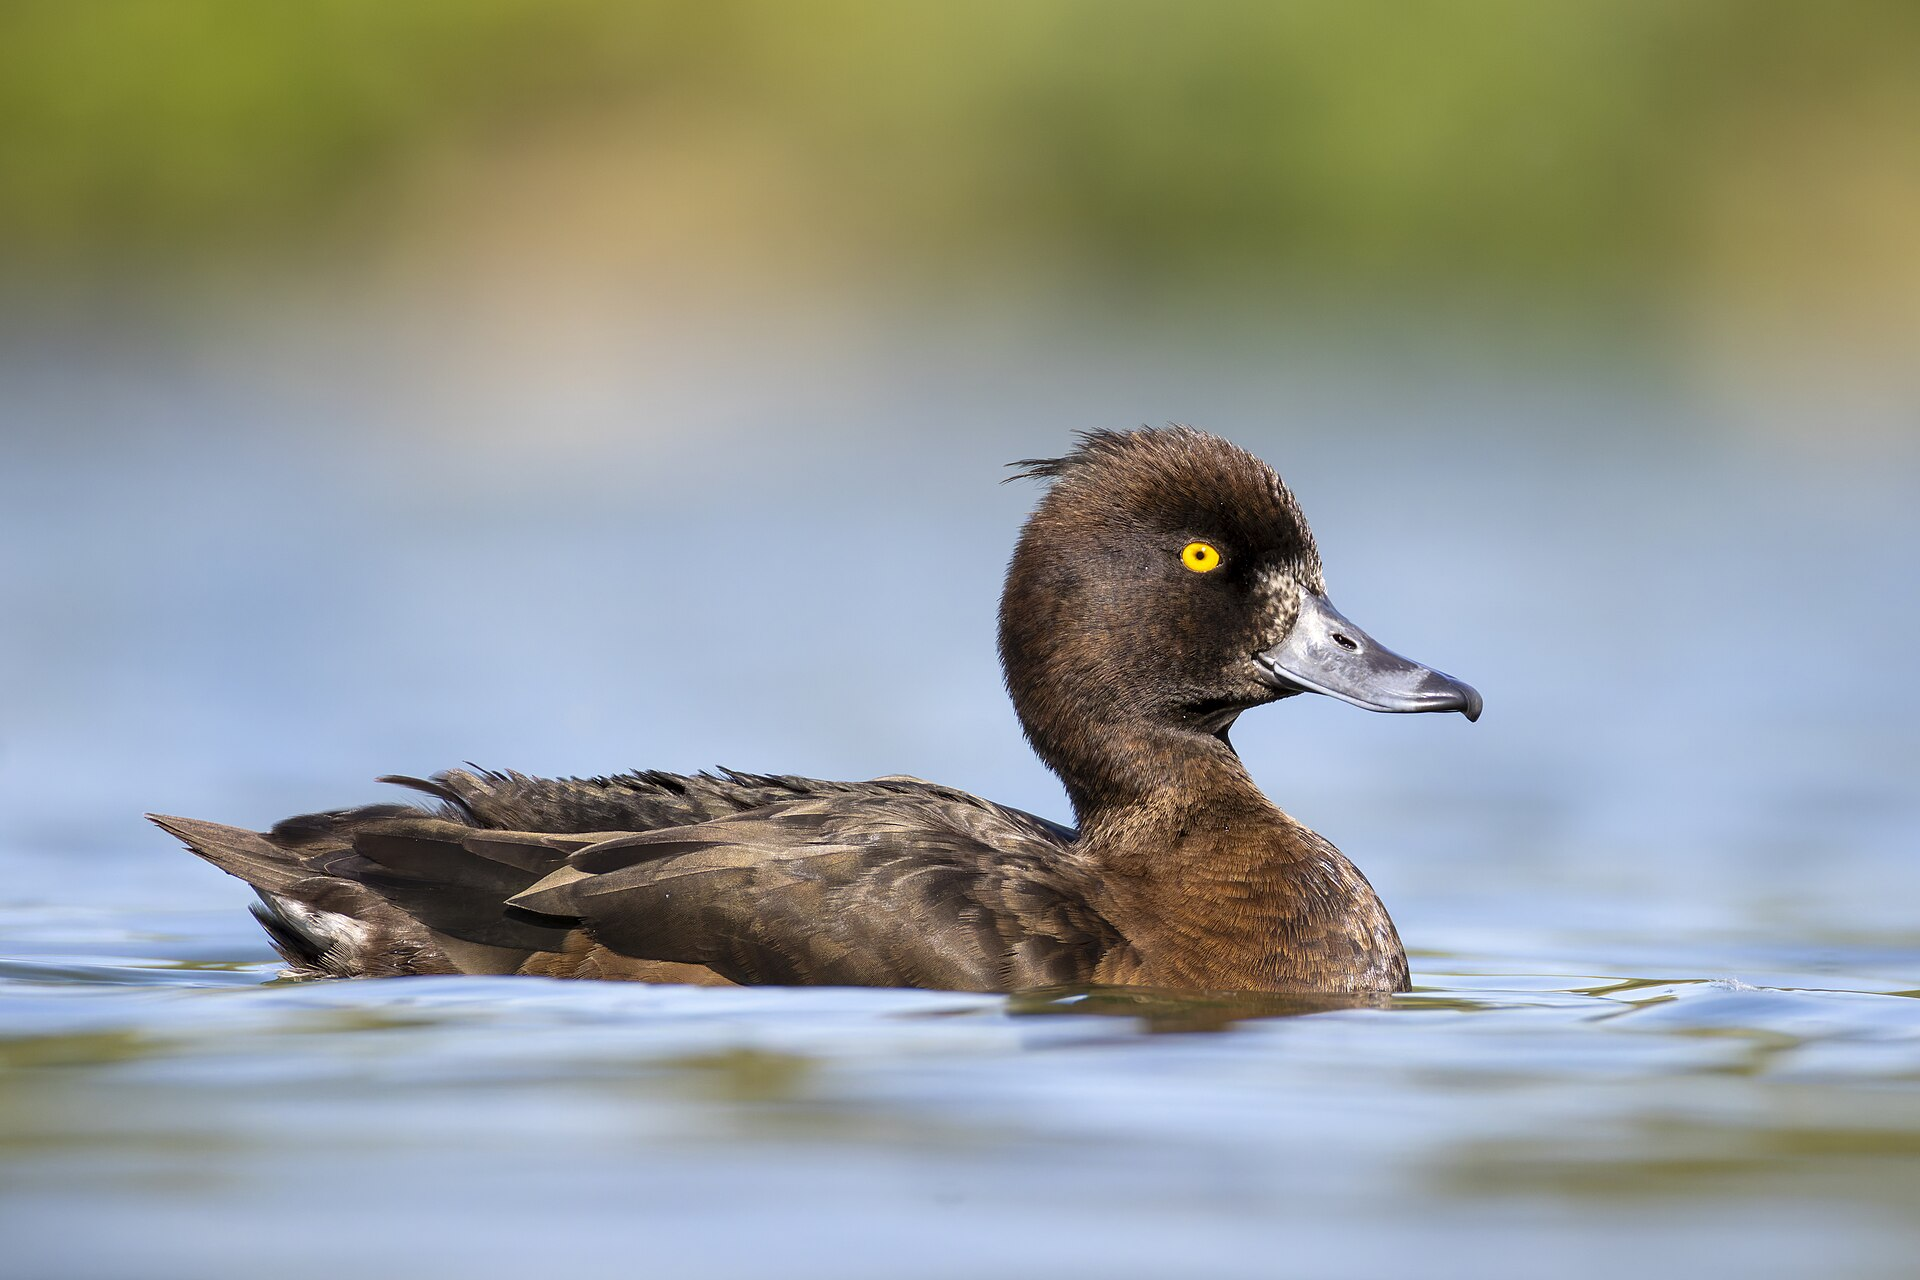
\includegraphics[width=0.7\linewidth, height=3cm, keepaspectratio]{Billeder/Dyr/Fugle/Aender/Dykaender/troldand_hun.jpg}
      \end{minipage}
    }%
    \vspace{0.05em}
    \footnotesize Andrik øverst, and nederst
  \end{columns}
\end{frame}

% ========== RØDHOVEDET AND ==========
\begin{frame}{%
  \begin{minipage}[c]{0.30\textwidth}
    Rødhovedet and
  \end{minipage}%
  \hfill
  \begin{minipage}[c]{0.45\textwidth}
    \footnotesize
    \textbf{Jagttid:} Ingen jagttid
  \end{minipage}%
  \hfill
  \begin{minipage}[c]{0.15\textwidth}
    \noindent\raggedleft
    
\includegraphics[width=0.5cm, height=0.5cm, keepaspectratio]{Billeder/Ikoner/star.png}
  \end{minipage}%
}
  \vspace{0.25em}
  \begin{columns}[T]
    % --- Venstre kolonne: Tekst ---
    \column{0.55\textwidth}
    \setlength{\parskip}{0.5em}
    \tiny
    \RaggedRight
    \textbf{\textit{Netta rufina}} – stor dykand der både fouragerer i og under overfladen \par
    \textbf{Udseende:}\\
    \quad – Andrik: Rødt hoved, skinnende rødt næb, sort bryst \par
    \quad – And: Mørkebrun med lidt lysere kinder, mørkt næb med rosa spids
    % --- Højre kolonne: Billeder ---
    \column{0.40\textwidth}
    \centering
    \fbox{%
      \begin{minipage}{\linewidth}
        \centering
        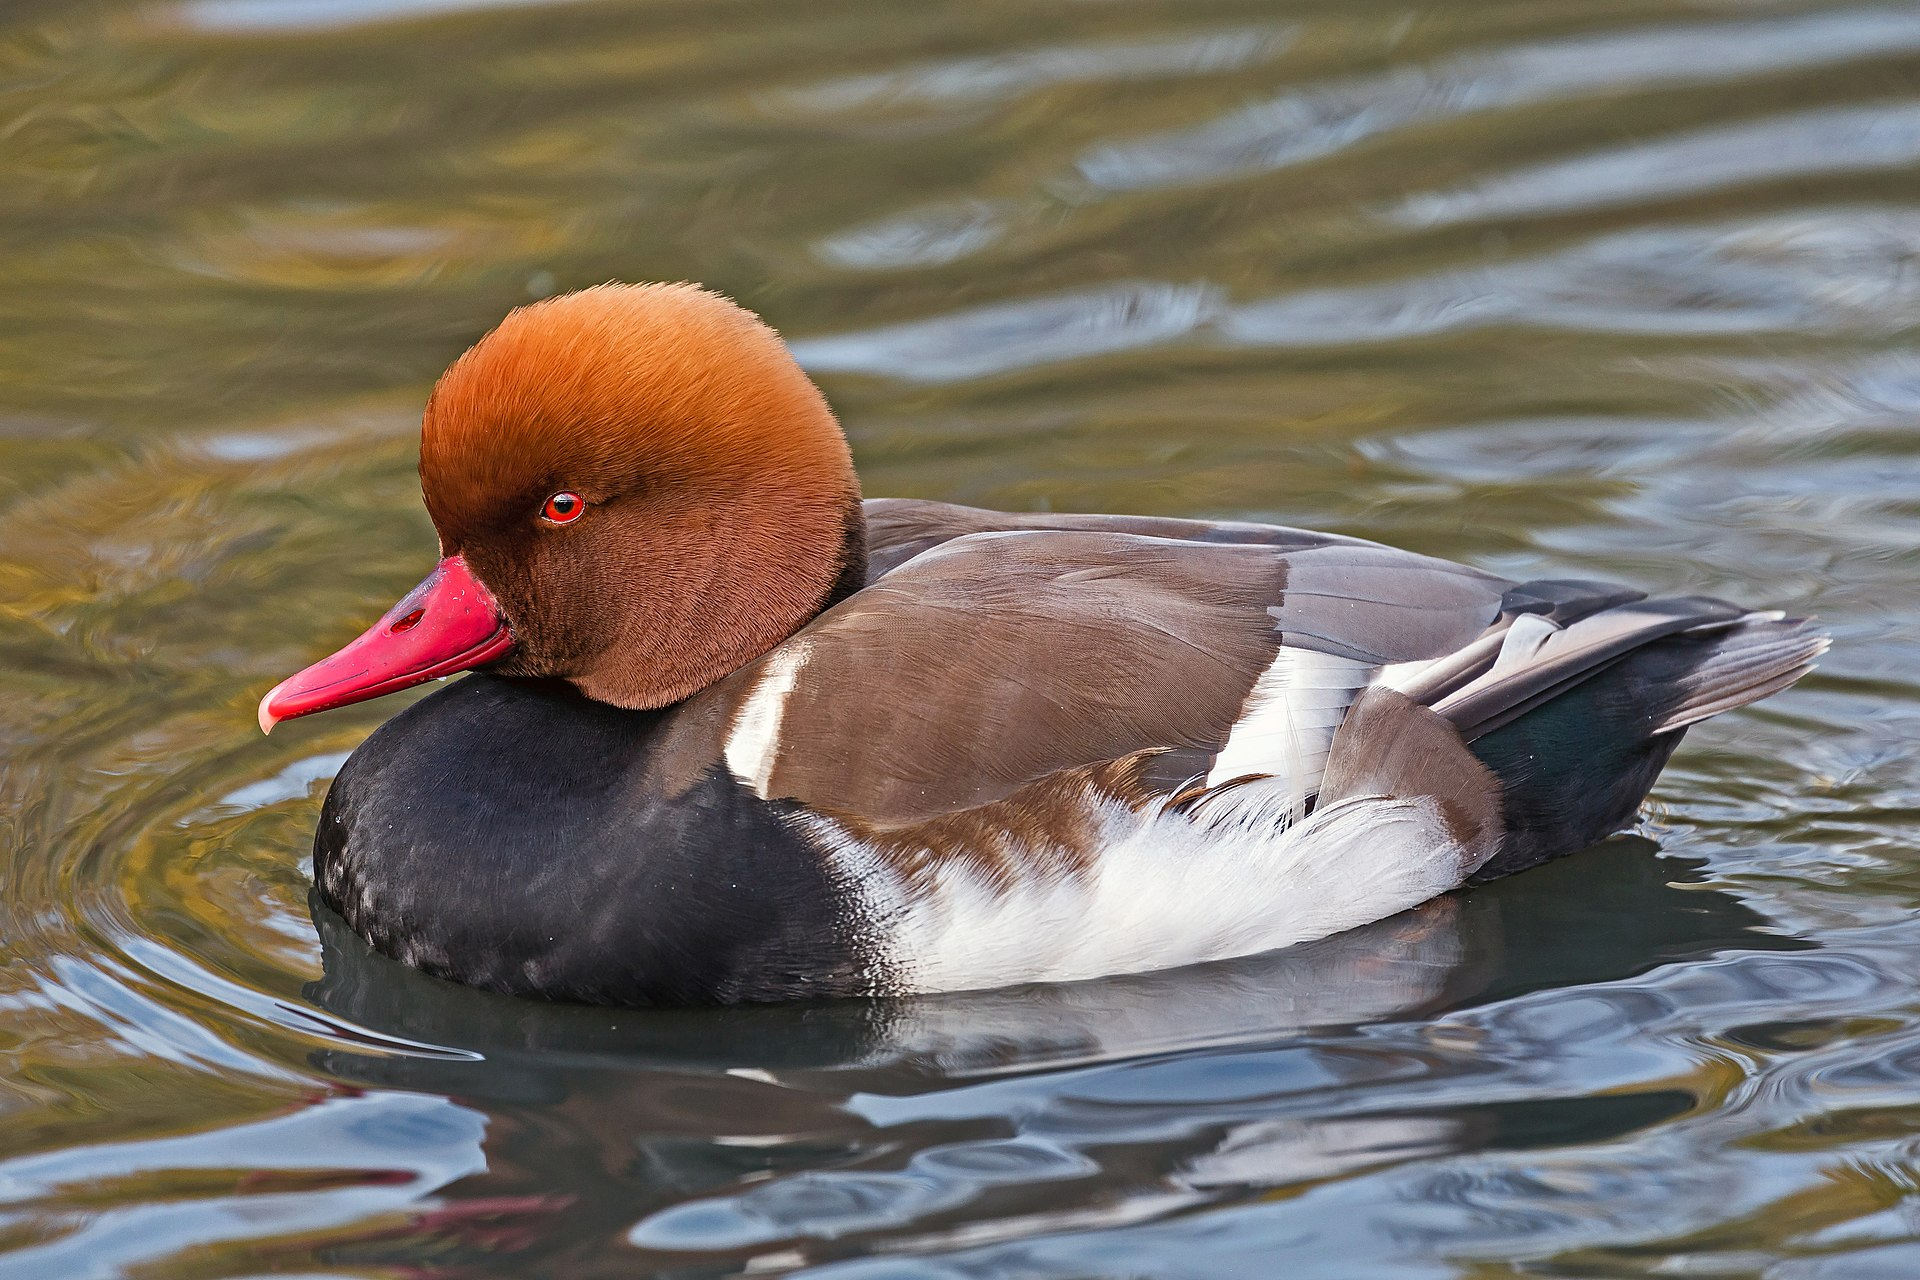
\includegraphics[width=0.7\linewidth, height=3cm, keepaspectratio]{Billeder/Dyr/Fugle/Aender/Dykaender/rødhovedetand_han.jpg}\\[0.5em]
        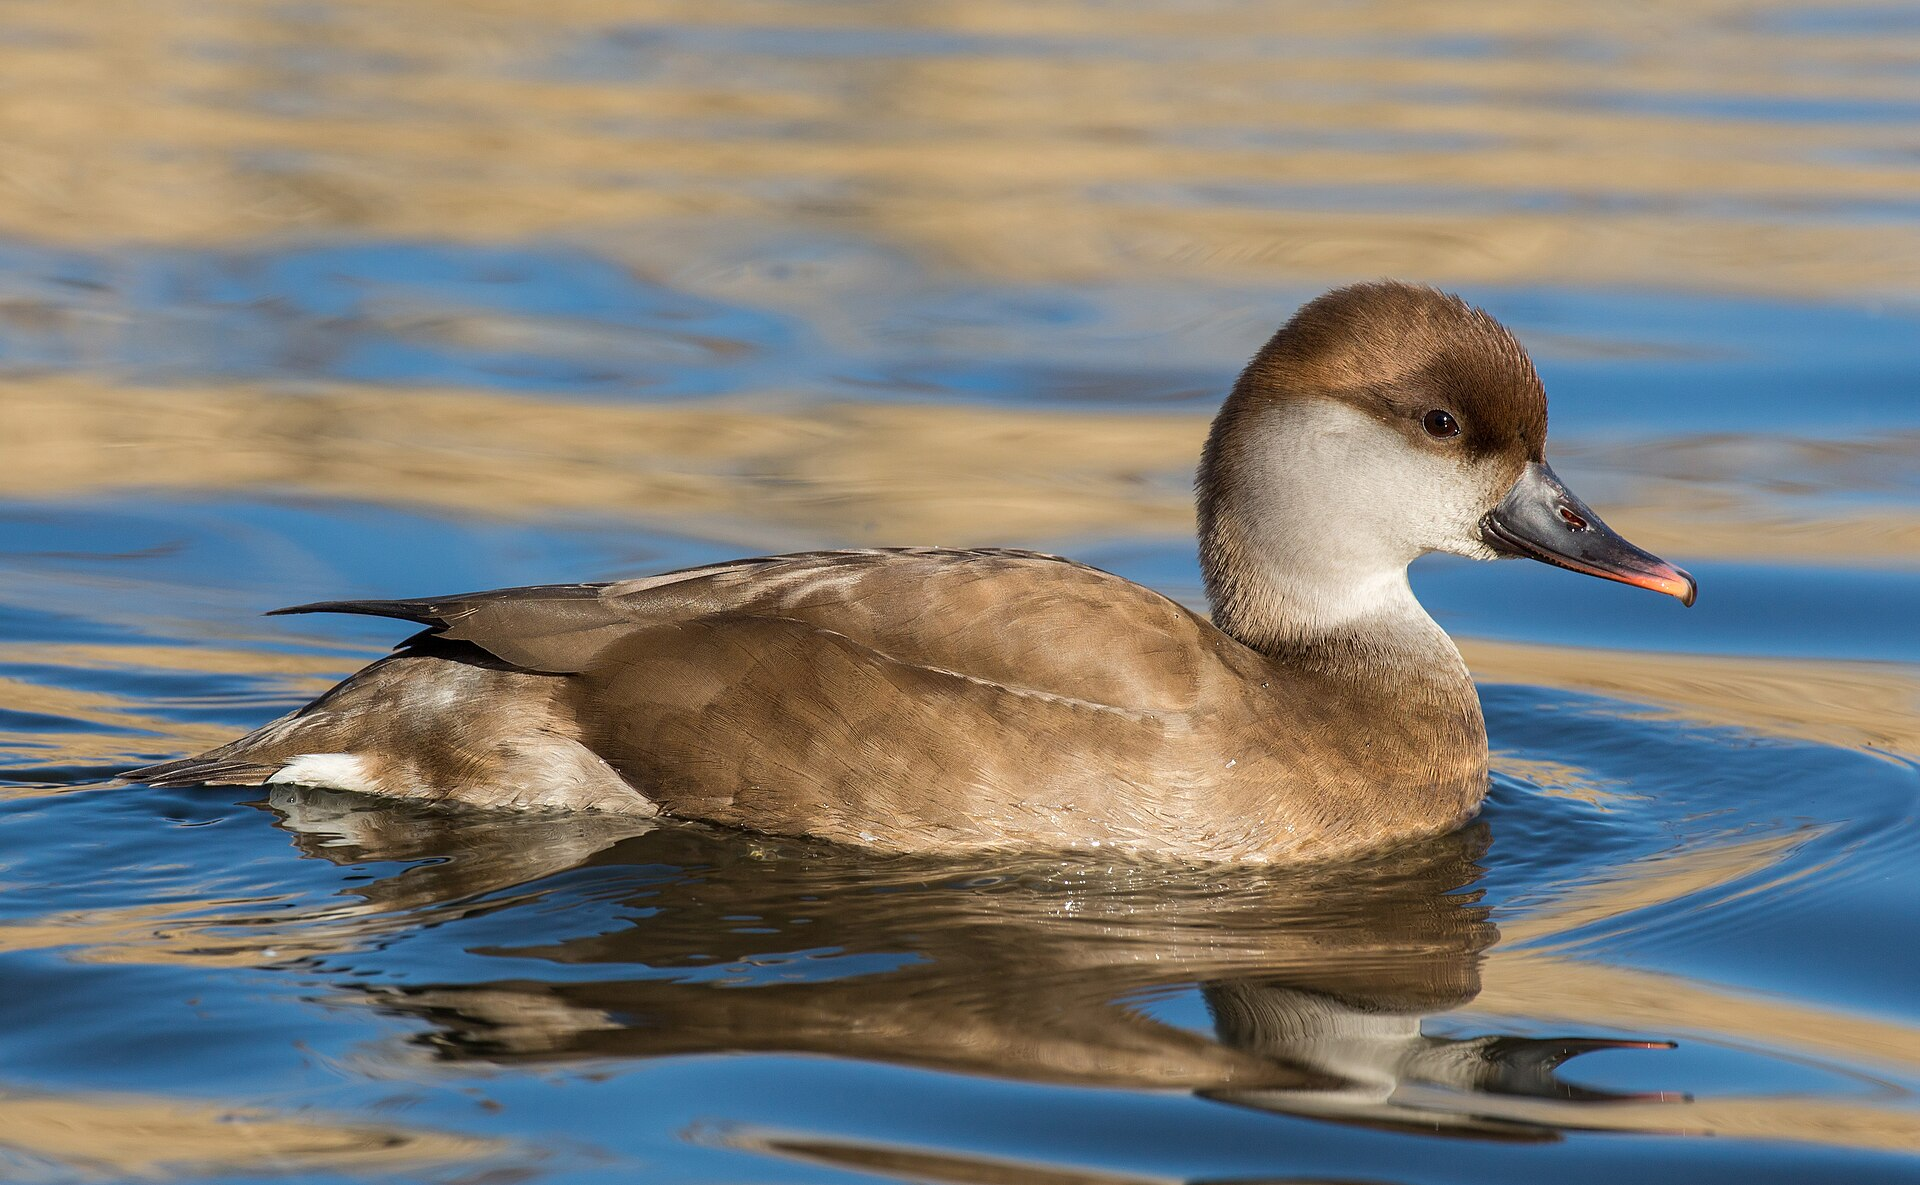
\includegraphics[width=0.7\linewidth, height=3cm, keepaspectratio]{Billeder/Dyr/Fugle/Aender/Dykaender/rødhovedetand_hun.jpg}
      \end{minipage}
    }%
    \vspace{0.05em}
    \footnotesize Andrik øverst, and nederst
  \end{columns}
\end{frame}

% ========== TAFFELAND ==========
\begin{frame}{%
  \begin{minipage}[c]{0.30\textwidth}
    Taffeland
  \end{minipage}%
  \hfill
  \begin{minipage}[c]{0.45\textwidth}
    \footnotesize
    \textbf{Jagttid:} Ingen jagttid
  \end{minipage}%
  \hfill
  \begin{minipage}[c]{0.15\textwidth}
    \noindent\raggedleft
    
\includegraphics[width=0.5cm, height=0.5cm, keepaspectratio]{Billeder/Ikoner/star.png}
  \end{minipage}%
}
  \vspace{0.25em}
  \begin{columns}[T]
    % --- Venstre kolonne: Tekst ---
    \column{0.55\textwidth}
    \setlength{\parskip}{0.5em}
    \tiny
    \RaggedRight
    \textbf{\textit{Aythya ferina}} – mellemstor dykand som opholder sig i ferske vande. Taffel = bord → for meget taffel = røde øjne \par
    \textbf{Udseende:}\\
    \quad – Andrik: Rødbrunt hoved, røde øjne \par
    \quad – And: Mørkebrun med gule aftegninger
    % --- Højre kolonne: Billeder ---
    \column{0.40\textwidth}
    \centering
    \fbox{%
      \begin{minipage}{\linewidth}
        \centering
        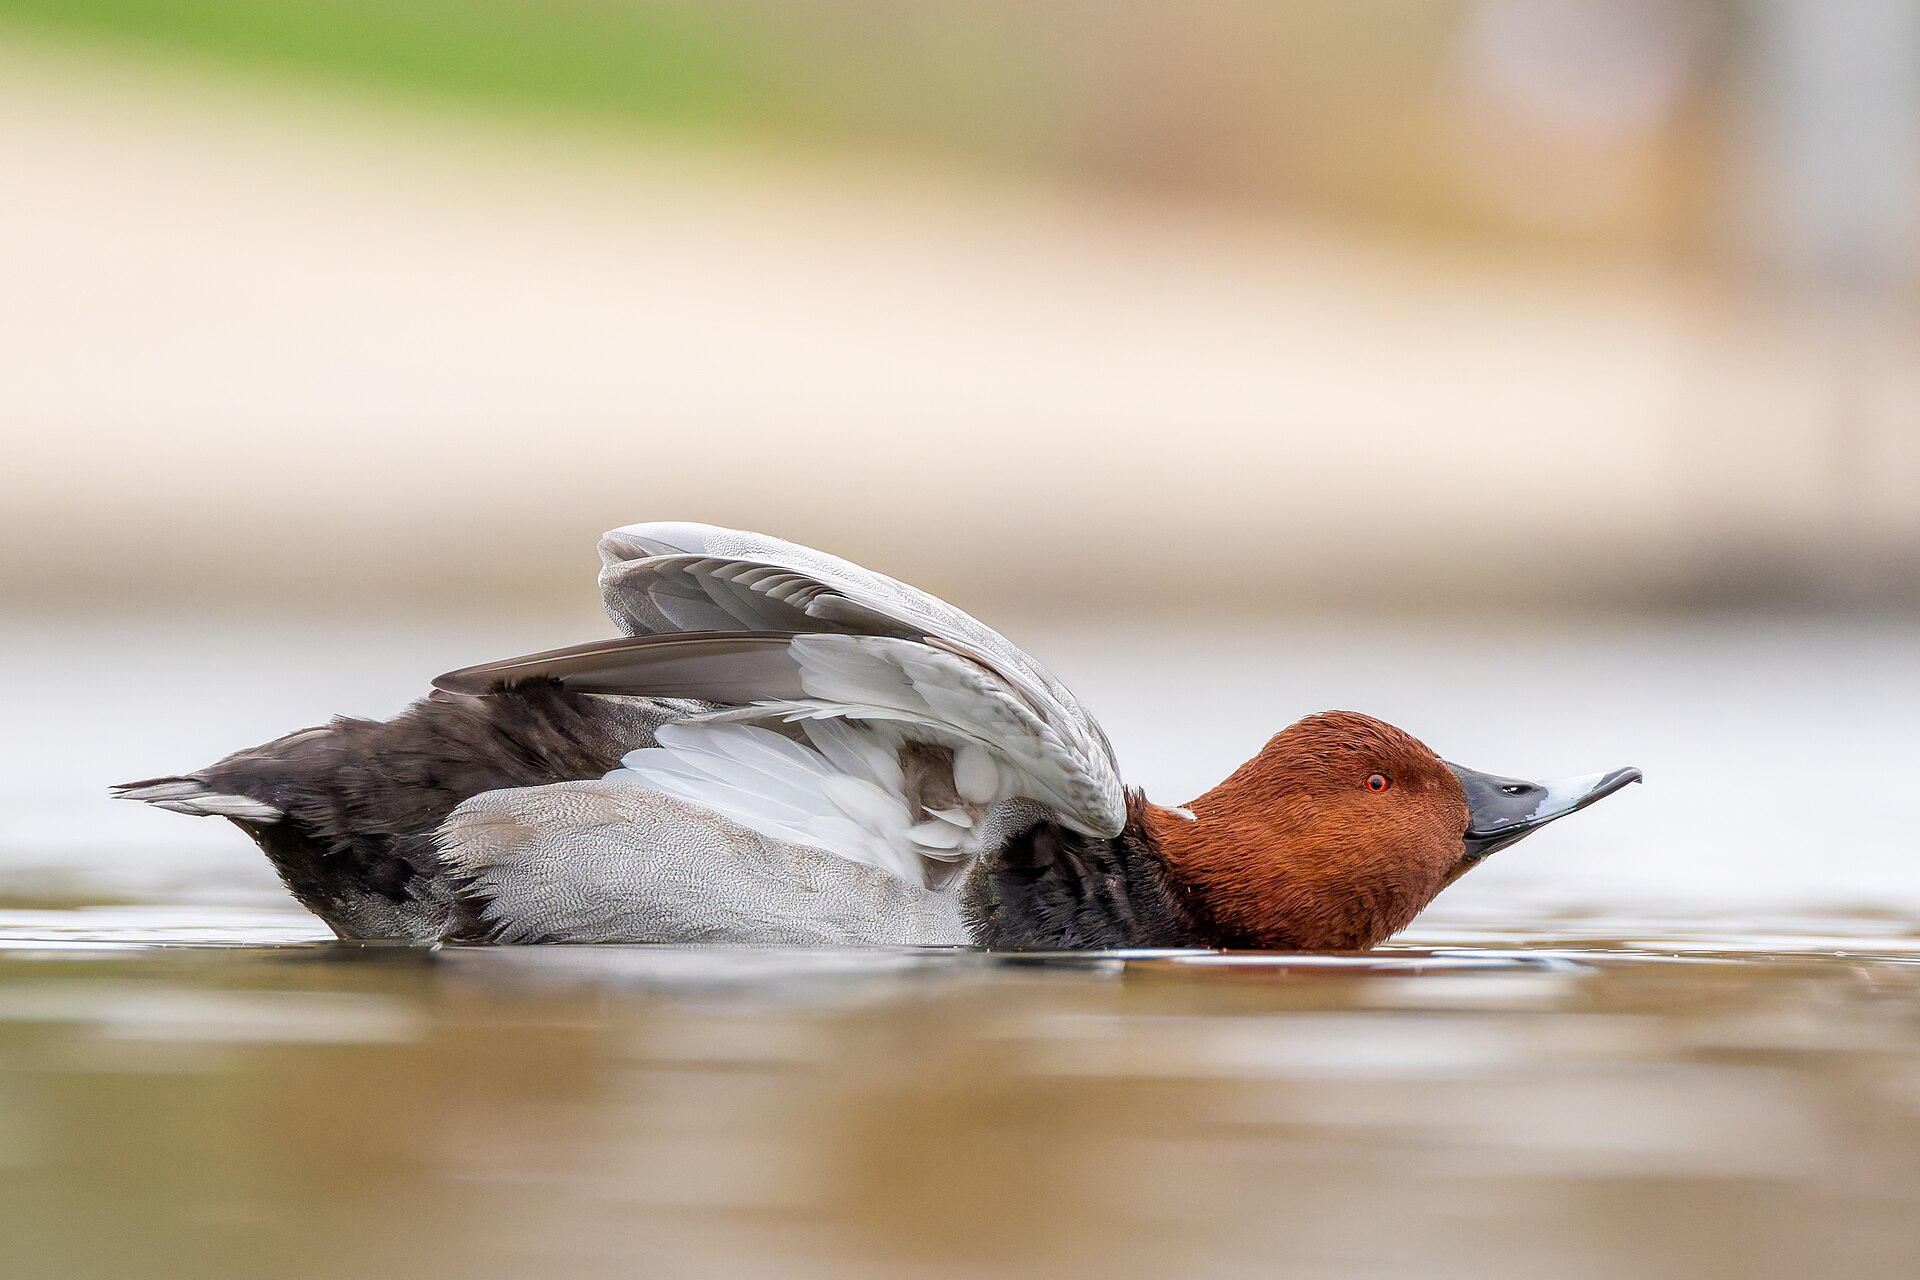
\includegraphics[width=0.7\linewidth, height=3cm, keepaspectratio]{Billeder/Dyr/Fugle/Aender/Dykaender/taffeland_han.jpg}\\[0.5em]
        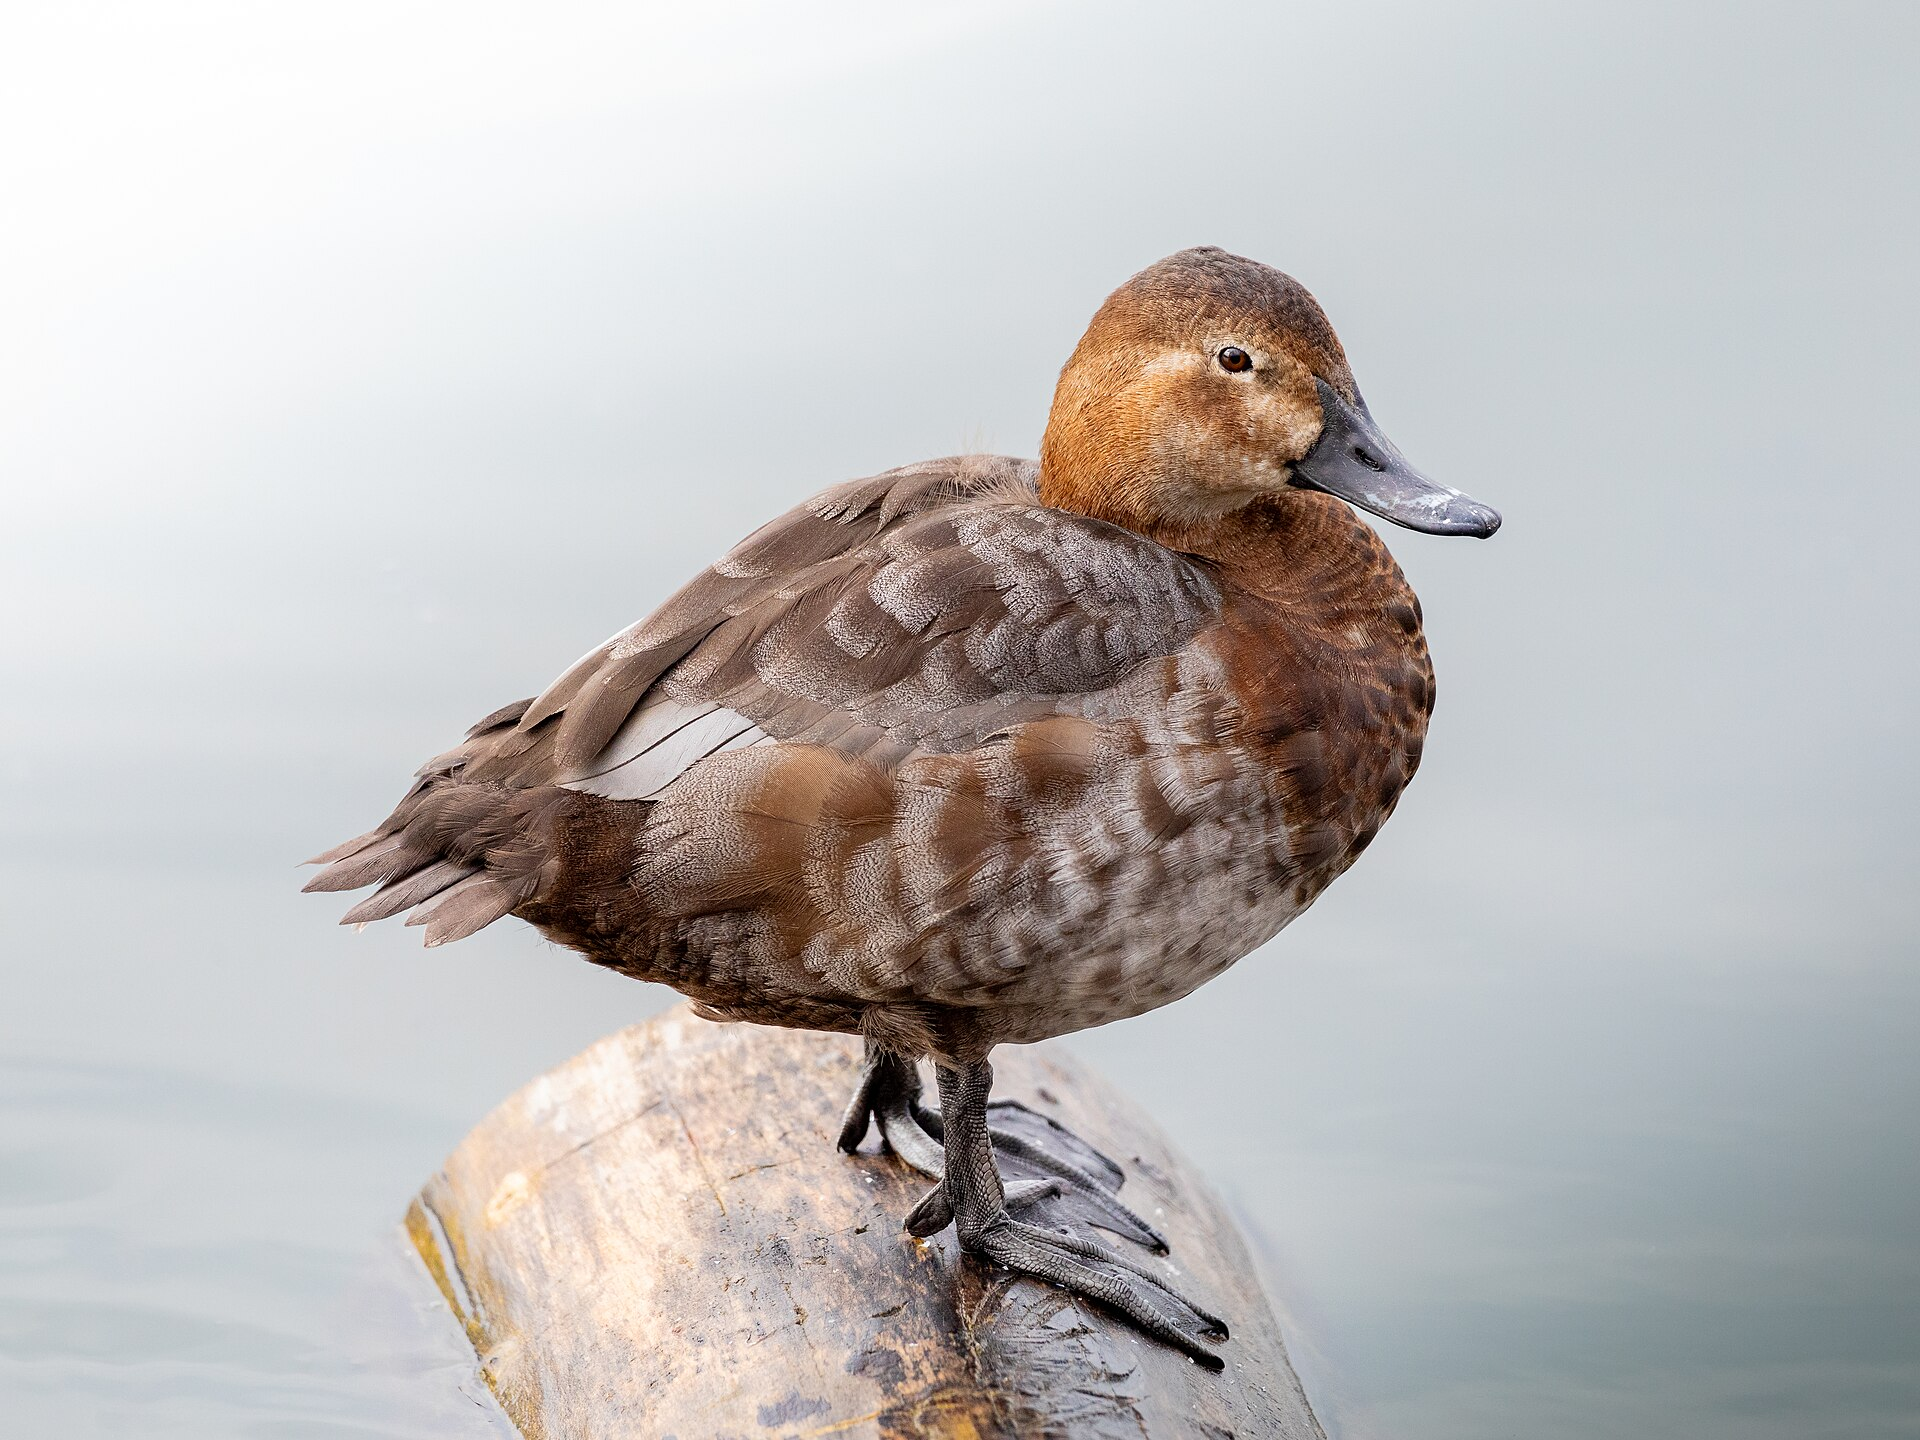
\includegraphics[width=0.7\linewidth, height=3cm, keepaspectratio]{Billeder/Dyr/Fugle/Aender/Dykaender/taffeland_hun.jpg}
      \end{minipage}
    }%
    \vspace{0.05em}
    \footnotesize Andrik øverst, and nederst
  \end{columns}
\end{frame}

% ========== BJERGAND ==========
\begin{frame}{%
  \begin{minipage}[t]{0.32\textwidth}
    Bjergand
  \end{minipage}%
  \hfill
  \begin{minipage}[t]{0.36\textwidth}
    \centering
    \footnotesize\textbf{Jagttid:} 1.\ oktober -- 31.\ januar
  \end{minipage}%
  \hfill
  \begin{minipage}[t]{0.15\textwidth}
    \noindent\raggedleft
    
\includegraphics[width=0.5cm, height=0.5cm, keepaspectratio]{Billeder/Ikoner/star.png}
  \end{minipage}%
}
  \vspace{0.25em}
  \begin{columns}[T]
    % --- Venstre kolonne: Tekst ---
    \column{0.55\textwidth}
    \setlength{\parskip}{0.5em}
    \tiny
    \RaggedRight
    \textbf{\textit{Aythya marila}} – mellemstor dykand der kan forveksles med troldand \par
    \textbf{Udseende:}\\
    \quad – Andrik: Sort hoved med grønligt skær, lysegrå ryg \par
    \quad – And: Hvid plet bag næbbet (ligner bjergtop med sne)
    % --- Højre kolonne: Billeder ---
    \column{0.40\textwidth}
    \centering
    \fbox{%
      \begin{minipage}{\linewidth}
        \centering
        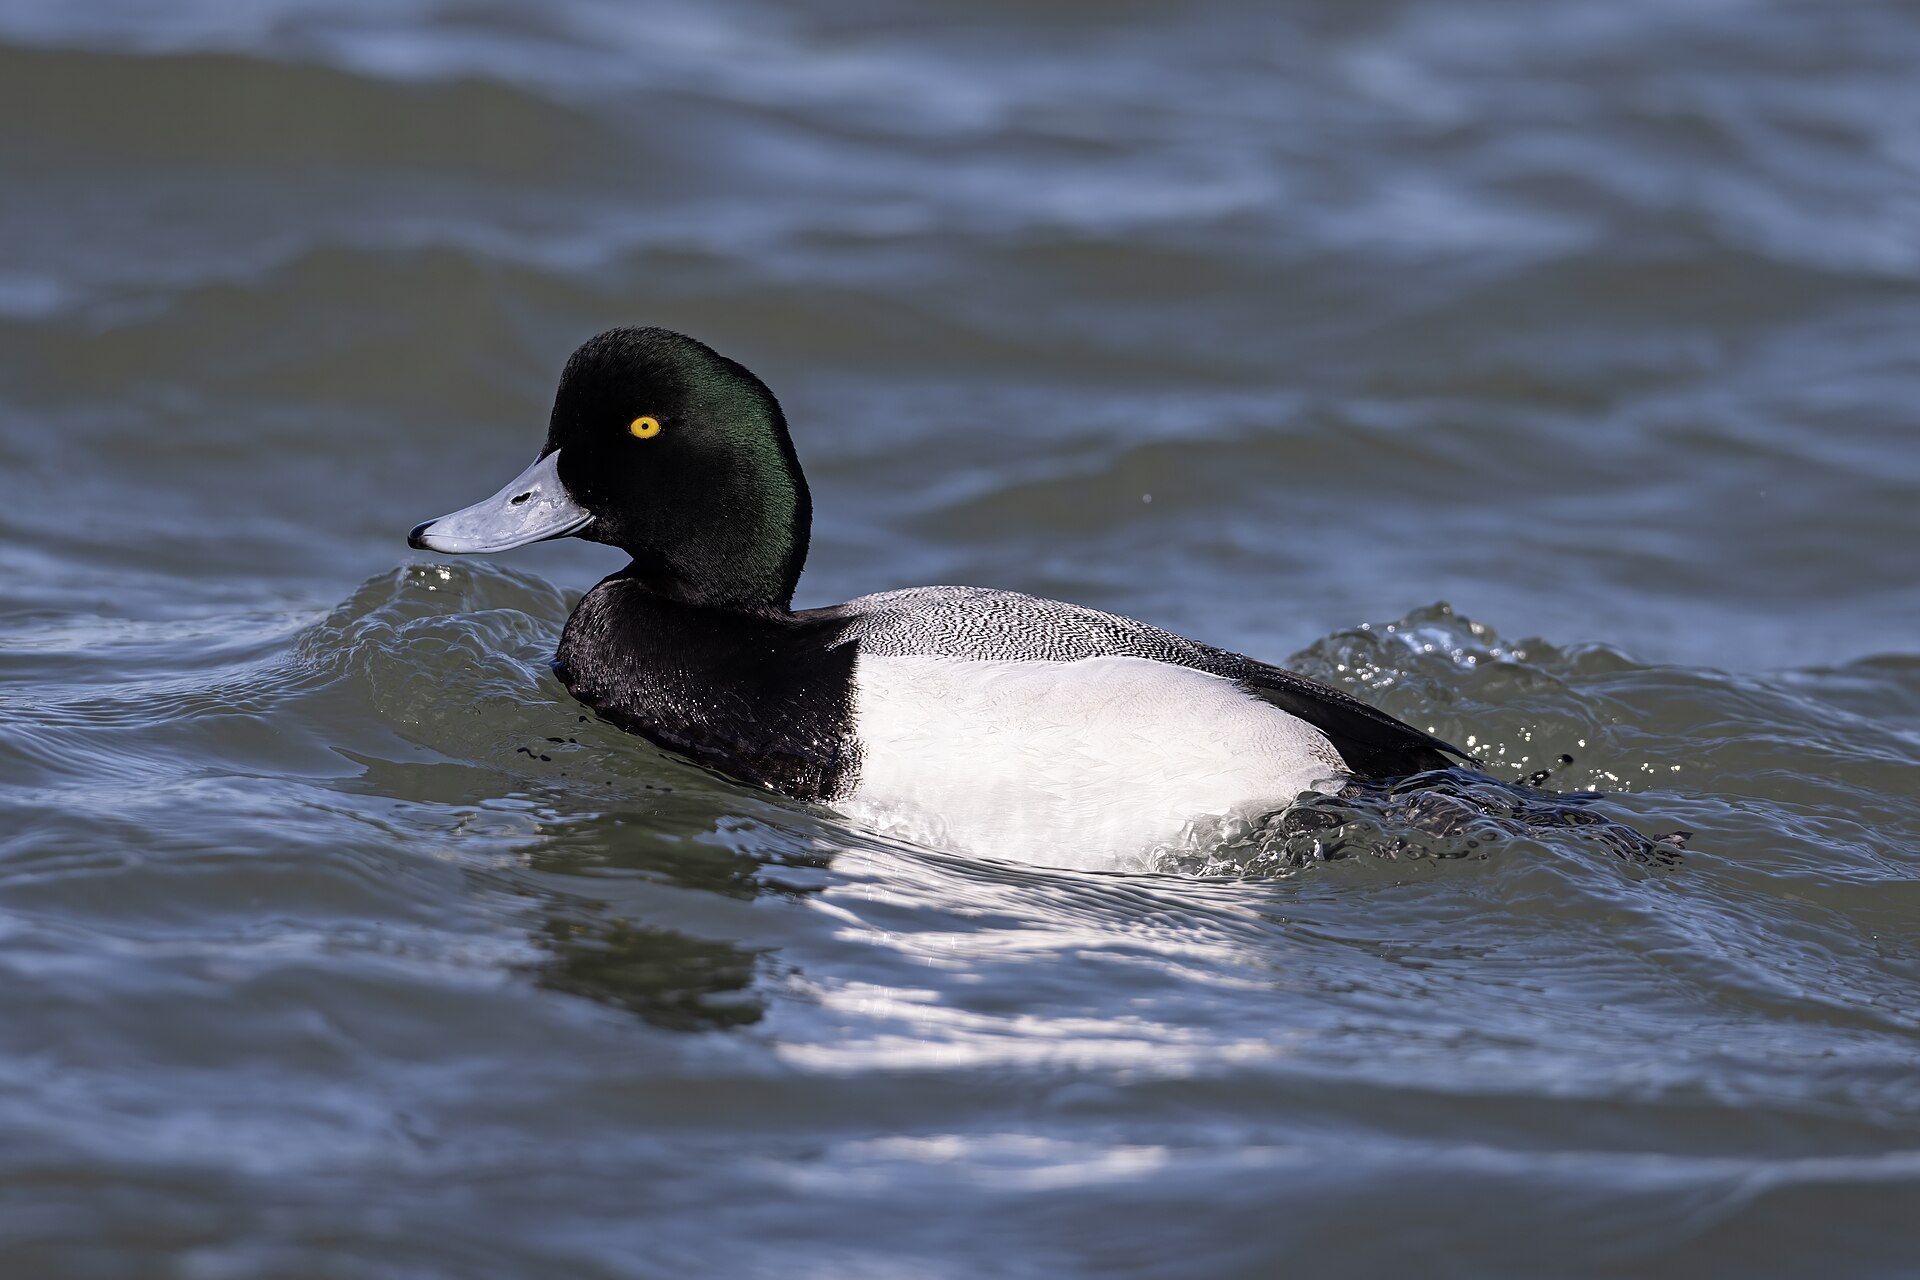
\includegraphics[width=0.7\linewidth, height=3cm, keepaspectratio]{Billeder/Dyr/Fugle/Aender/Dykaender/bjergand_han.jpg}\\[0.5em]
        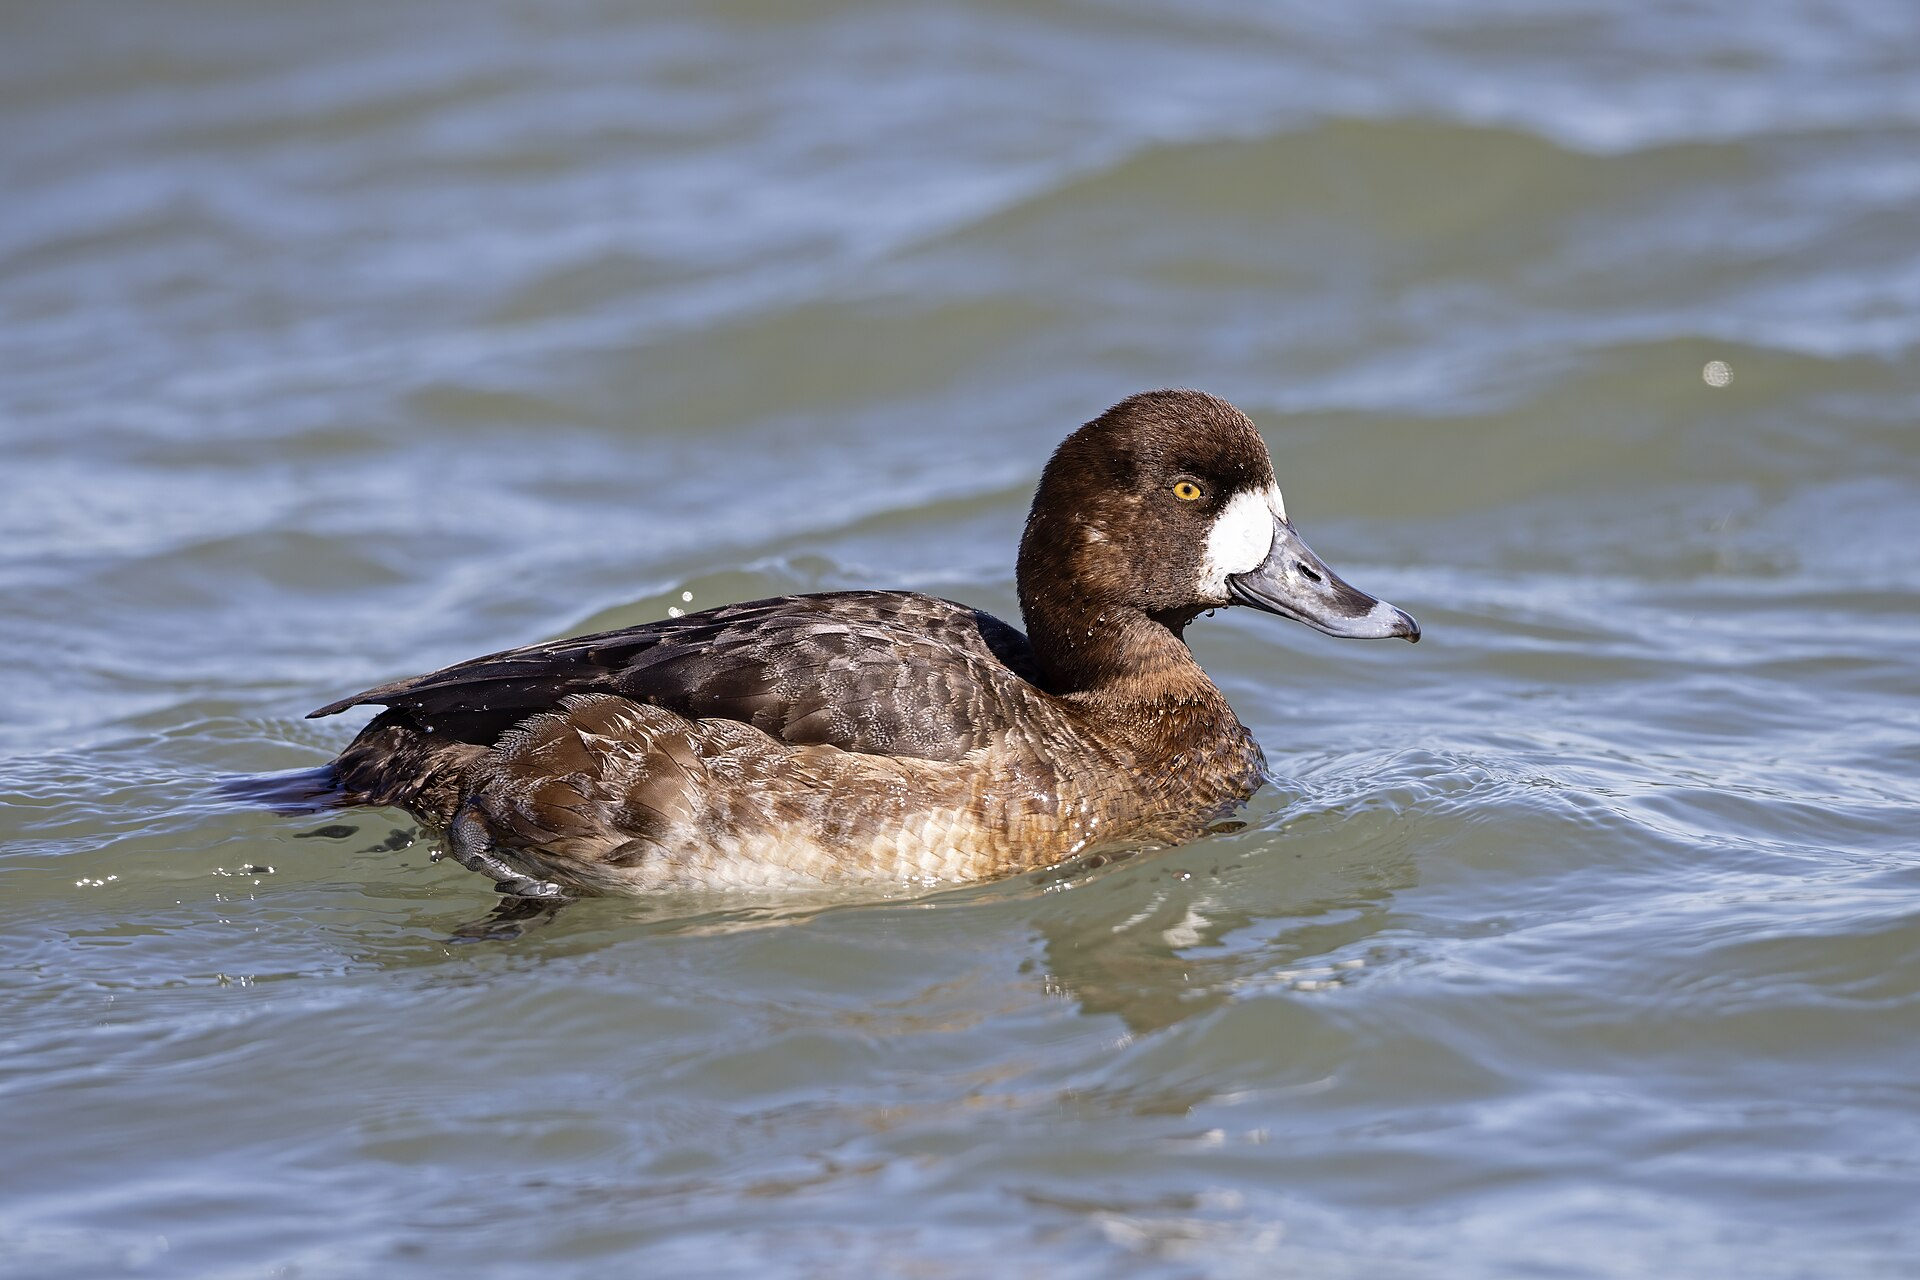
\includegraphics[width=0.7\linewidth, height=3cm, keepaspectratio]{Billeder/Dyr/Fugle/Aender/Dykaender/bjergand_hun.jpg}%
      \end{minipage}
    }%
    \vspace{0.05em}
    \footnotesize Andrik øverst, and nederst
  \end{columns}
\end{frame}

% ========== HAVLIT ==========
\begin{frame}{%
  \begin{minipage}[t]{0.32\textwidth}
    Havlit
  \end{minipage}%
  \hfill
  \begin{minipage}[t]{0.36\textwidth}
    \centering
    \footnotesize\textbf{Jagttid:} Ingen jagttid
  \end{minipage}%
  \hfill
  \begin{minipage}[t]{0.15\textwidth}
    \noindent\raggedleft
    
\includegraphics[width=0.5cm, height=0.5cm, keepaspectratio]{Billeder/Ikoner/star.png}
  \end{minipage}%
}
  \vspace{0.25em}
  \begin{columns}[T]
    % --- Venstre kolonne: Tekst ---
    \column{0.55\textwidth}
    \setlength{\parskip}{0.5em}
    \tiny
    \RaggedRight
    \textbf{\textit{Clangula hyemalis}} – lille dykand med meget lang hale \par
    \textbf{Udseende:}\\
    \quad – Andrik: Brun, sort, hvid med meget lange halefjer \par
    \quad – And: Hvid, brun spraglet, kort kraftigt næb
    % --- Højre kolonne: Billeder ---
    \column{0.40\textwidth}
    \centering
    \fbox{%
      \begin{minipage}{\linewidth}
        \centering
        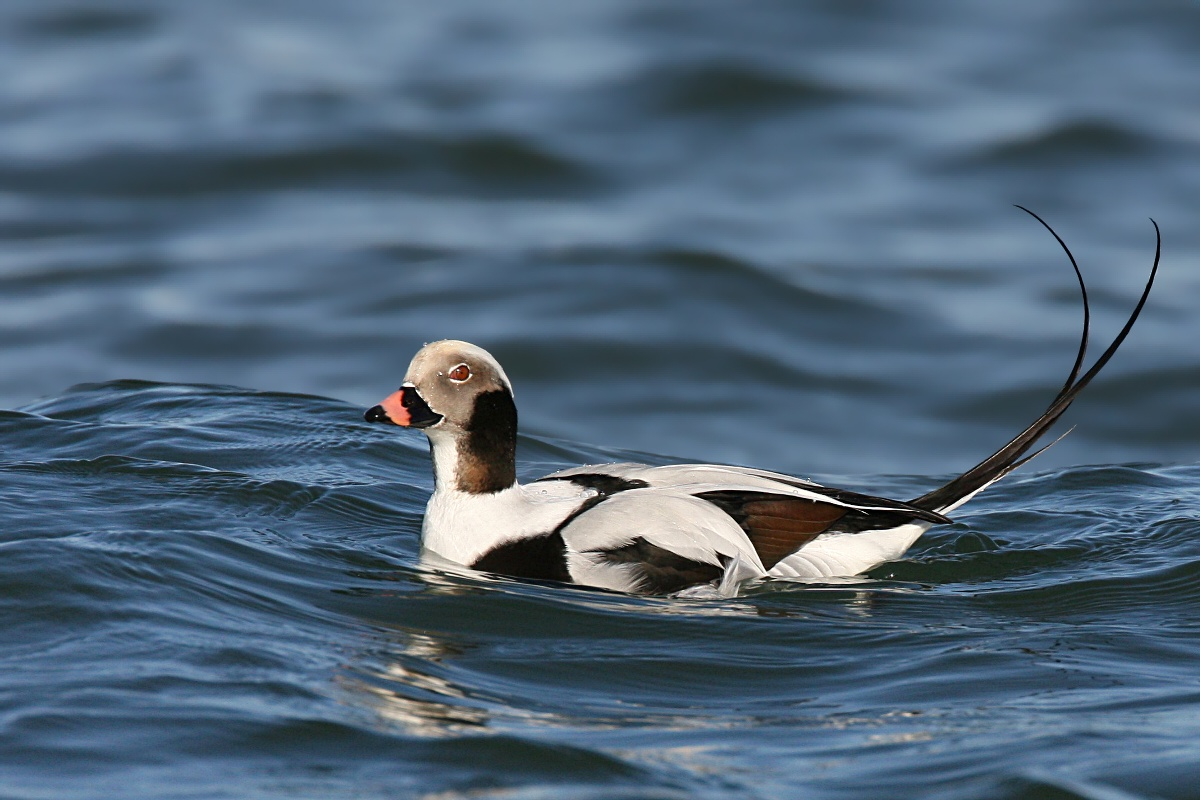
\includegraphics[width=0.7\linewidth, height=3cm, keepaspectratio]{Billeder/Dyr/Fugle/Aender/Dykaender/havlit_han.jpg}\\[0.5em]
        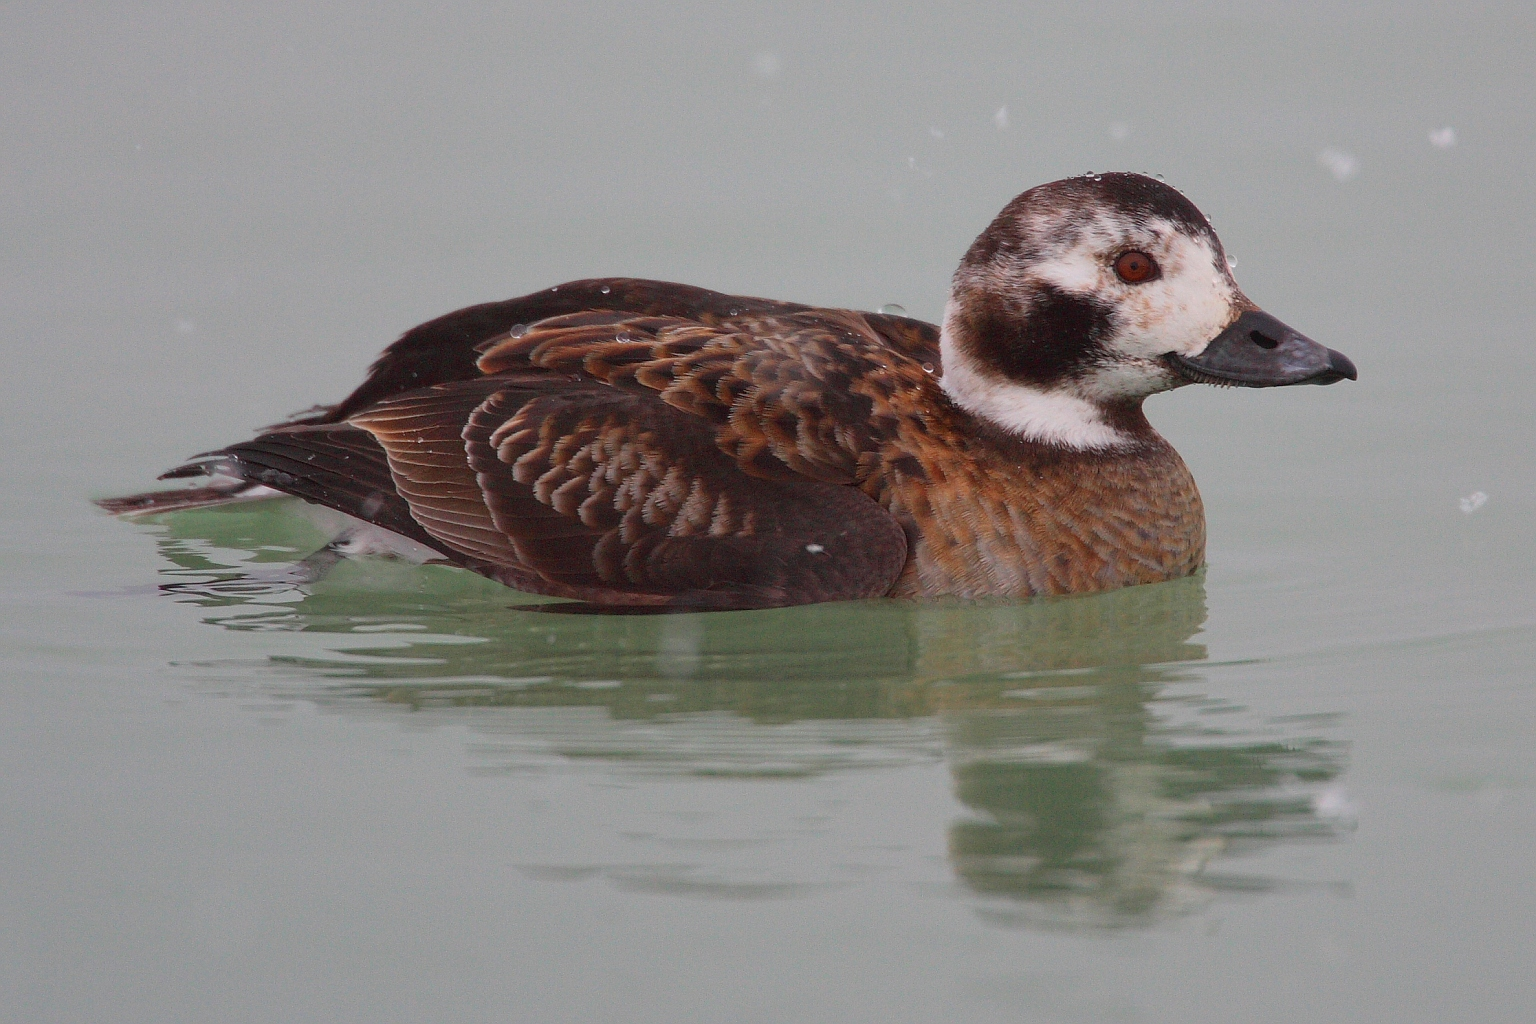
\includegraphics[width=0.7\linewidth, height=3cm, keepaspectratio]{Billeder/Dyr/Fugle/Aender/Dykaender/havlit_hun.jpg}%
      \end{minipage}
    }%
    \vspace{0.05em}
    \footnotesize Andrik øverst, and nederst
  \end{columns}
\end{frame}

% ========== SORTAND ==========
\begin{frame}{%
  \begin{minipage}[t]{0.32\textwidth}
    Sortand
  \end{minipage}%
  \hfill
  \begin{minipage}[t]{0.36\textwidth}
    \centering
    \footnotesize\textbf{Jagttid:} 1.\ oktober -- 31.\ januar
  \end{minipage}%
  \hfill
  \begin{minipage}[t]{0.15\textwidth}
    \noindent\raggedleft
    
\includegraphics[width=0.5cm, height=0.5cm, keepaspectratio]{Billeder/Ikoner/star.png}
  \end{minipage}%
}
  \vspace{0.25em}
  \begin{columns}[T]
    % --- Venstre kolonne: Tekst ---
    \column{0.55\textwidth}
    \setlength{\parskip}{0.5em}
    \tiny
    \RaggedRight
    \textbf{\textit{Melanitta nigra}} – mellemstor kompakt dykand – lever på havet \par
    \textbf{Udseende:}\\
    \quad – Andrik: Ensfarvet sort, orange knop inderst på næbbet \par
    \quad – And: Ensfarvet mørkbrun med lysebrun halsplet
    % --- Højre kolonne: Billeder ---
    \column{0.40\textwidth}
    \centering
    \fbox{%
      \begin{minipage}{\linewidth}
        \centering
        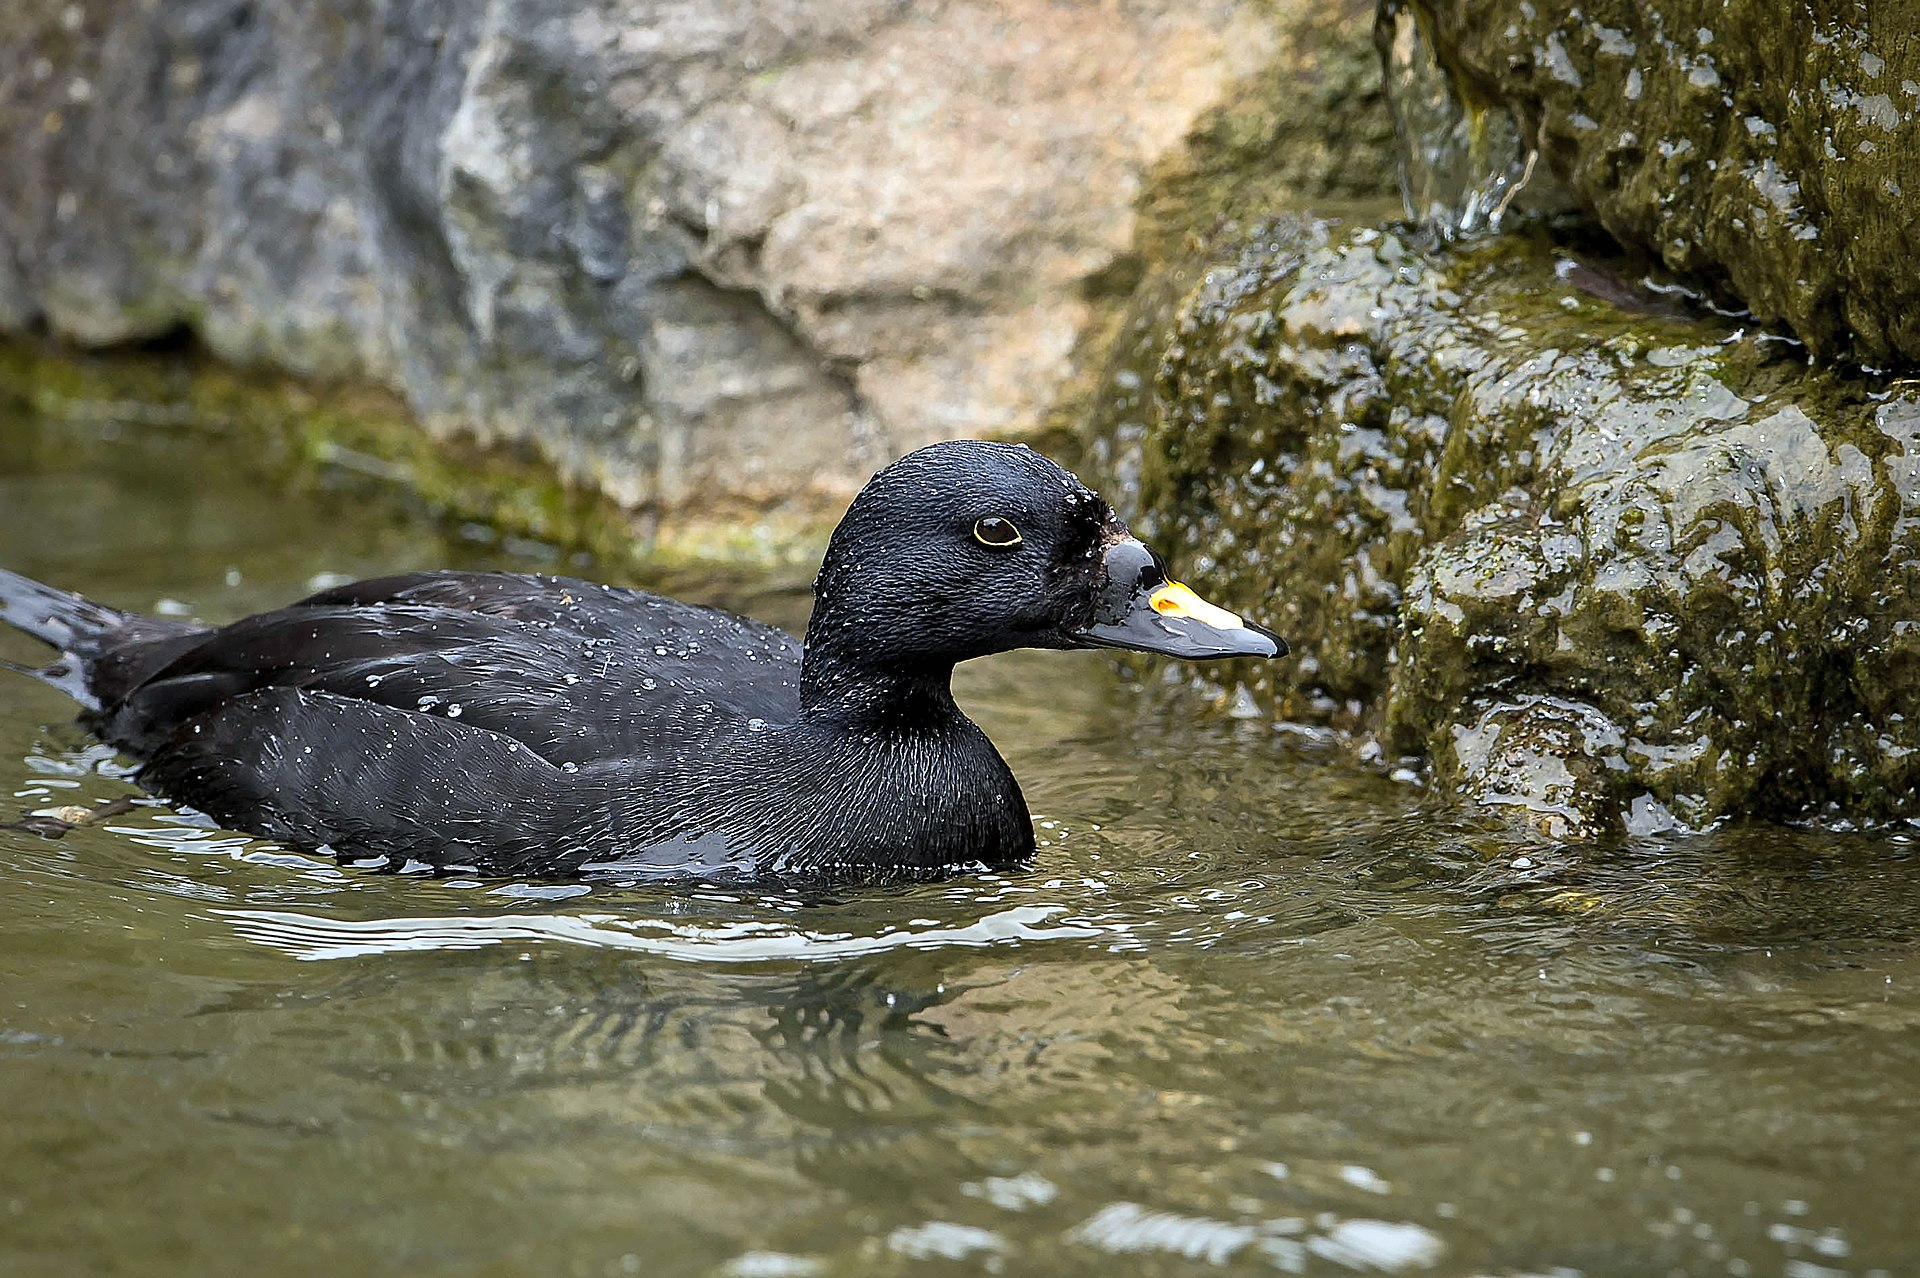
\includegraphics[width=0.7\linewidth, height=3cm, keepaspectratio]{Billeder/Dyr/Fugle/Aender/Dykaender/sortand_han.jpg}\\[0.5em]
        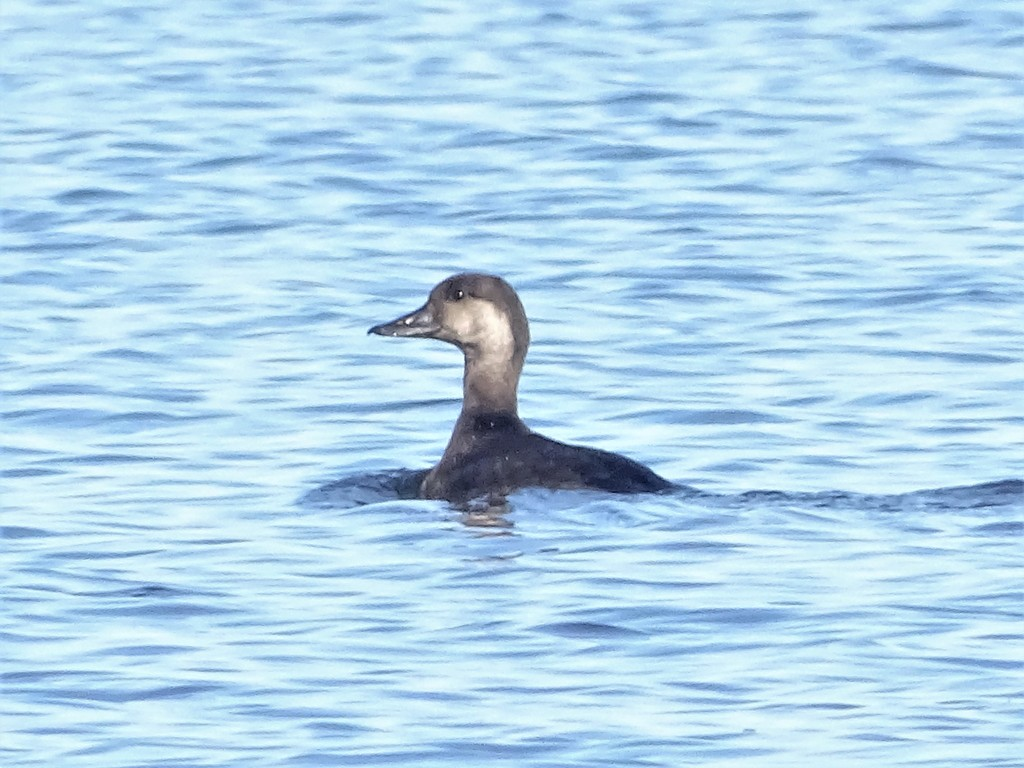
\includegraphics[width=0.7\linewidth, height=3cm, keepaspectratio]{Billeder/Dyr/Fugle/Aender/Dykaender/sortand_hun.jpg}%
      \end{minipage}
    }%
    \vspace{0.05em}
    \footnotesize Andrik øverst, and nederst
  \end{columns}
\end{frame}

% ========== FLØJLSAND ==========
\begin{frame}{%
  \begin{minipage}[t]{0.32\textwidth}
    Fløjlsand
  \end{minipage}%
  \hfill
  \begin{minipage}[t]{0.36\textwidth}
    \centering
    \footnotesize\textbf{Jagttid:} Ingen jagttid
  \end{minipage}%
  \hfill
  \begin{minipage}[t]{0.15\textwidth}
    \noindent\raggedleft
    
\includegraphics[width=0.5cm, height=0.5cm, keepaspectratio]{Billeder/Ikoner/star.png}
  \end{minipage}%
}
  \vspace{0.25em}
  \begin{columns}[T]
    % --- Venstre kolonne: Tekst ---
    \column{0.55\textwidth}
    \setlength{\parskip}{0.5em}
    \tiny
    \RaggedRight
    \textbf{\textit{Melanitta fusca}} – mellemstor kraftig dykand \par
    \textbf{Udseende:}\\
    \quad – Andrik: Sort krop med hvide fjer på vinger \par
    \quad – And: Mørk med hvidt vingespejl og plet bag næbbet
    % --- Højre kolonne: Billeder ---
    \column{0.40\textwidth}
    \centering
    \fbox{%
      \begin{minipage}{\linewidth}
        \centering
        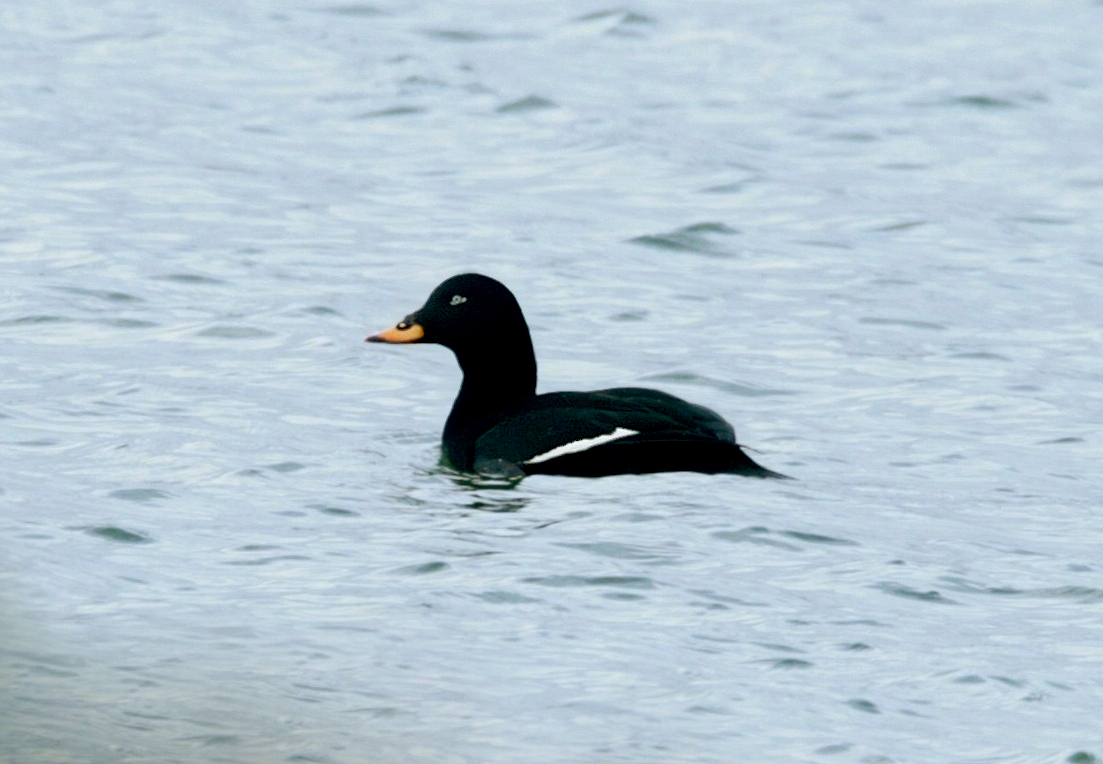
\includegraphics[width=0.7\linewidth, height=3cm, keepaspectratio]{Billeder/Dyr/Fugle/Aender/Dykaender/fløjlsand_han.jpg}\\[0.5em]
        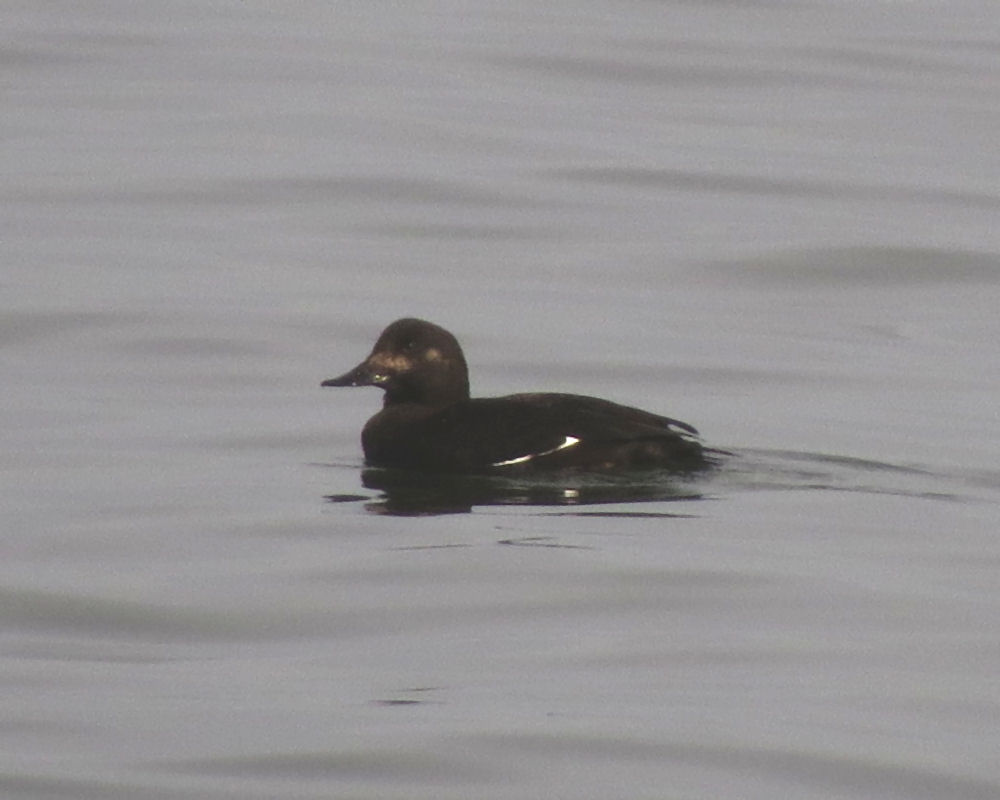
\includegraphics[width=0.7\linewidth, height=3cm, keepaspectratio]{Billeder/Dyr/Fugle/Aender/Dykaender/fløjlsand_hun.jpg}%
      \end{minipage}
    }%
    \vspace{0.05em}
    \footnotesize Andrik øverst, and nederst
  \end{columns}
\end{frame}

% ========== AMERIKANSK SKARVEAND ==========
\begin{frame}{%
  \begin{minipage}[c]{0.30\textwidth}
    Amerikansk \\ skarveand
  \end{minipage}%
  \hfill
  \begin{minipage}[c]{0.45\textwidth}
    \footnotesize
    \textbf{Jagttid:} Ingen jagttid \\
    \textbf{Regulering:} Uden aftale: Hele året (invasiv)
  \end{minipage}%
  \hfill
  \begin{minipage}[c]{0.15\textwidth}
    \noindent\raggedleft
    
\includegraphics[width=0.5cm, height=0.5cm, keepaspectratio]{Billeder/Ikoner/star.png}
  \end{minipage}%
}
  \vspace{0.25em}
  \begin{columns}[T]
    % --- Venstre kolonne: Tekst ---
    \column{0.55\textwidth}
    \setlength{\parskip}{0.5em}
    \tiny
    \RaggedRight
    \textbf{\textit{Oxyura jamaicensis}} – meget lille dykand som er klassificeret som invasiv \par
    \textbf{Udseende:}\\
    \quad – Andrik: Hvide kinder, lyseblåt næb \par
    \quad – And: Brunplettet, lille spids hale
    % --- Højre kolonne: Billeder ---
    \column{0.40\textwidth}
    \centering
    \fbox{%
      \begin{minipage}{\linewidth}
        \centering
        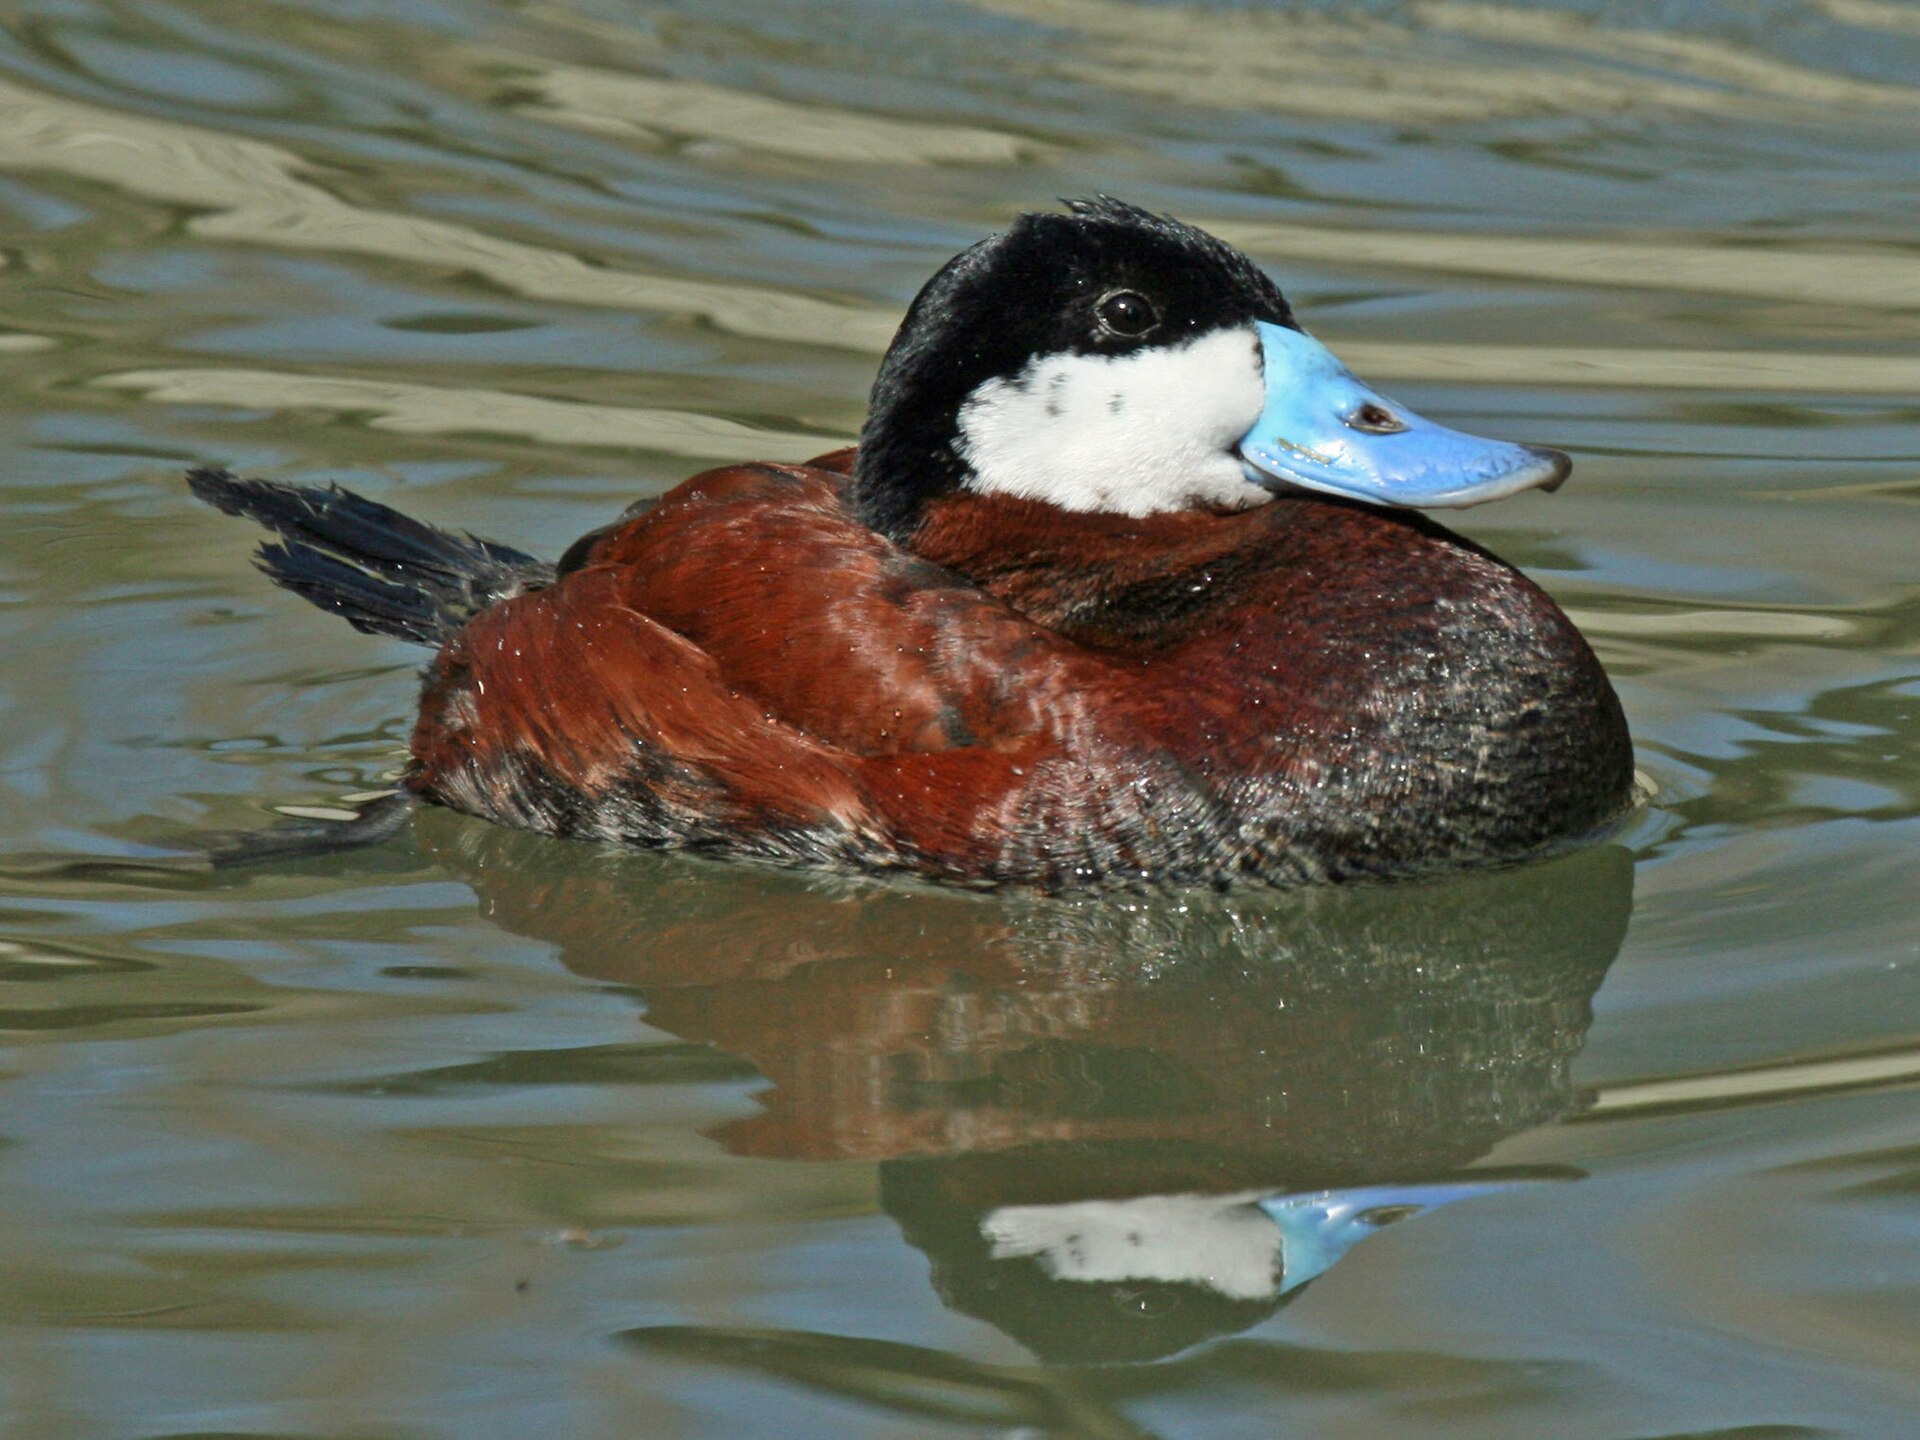
\includegraphics[width=0.7\linewidth, height=3cm, keepaspectratio]{Billeder/Dyr/Fugle/Aender/Dykaender/am_skarveand_han.jpg}\\[0.5em]
        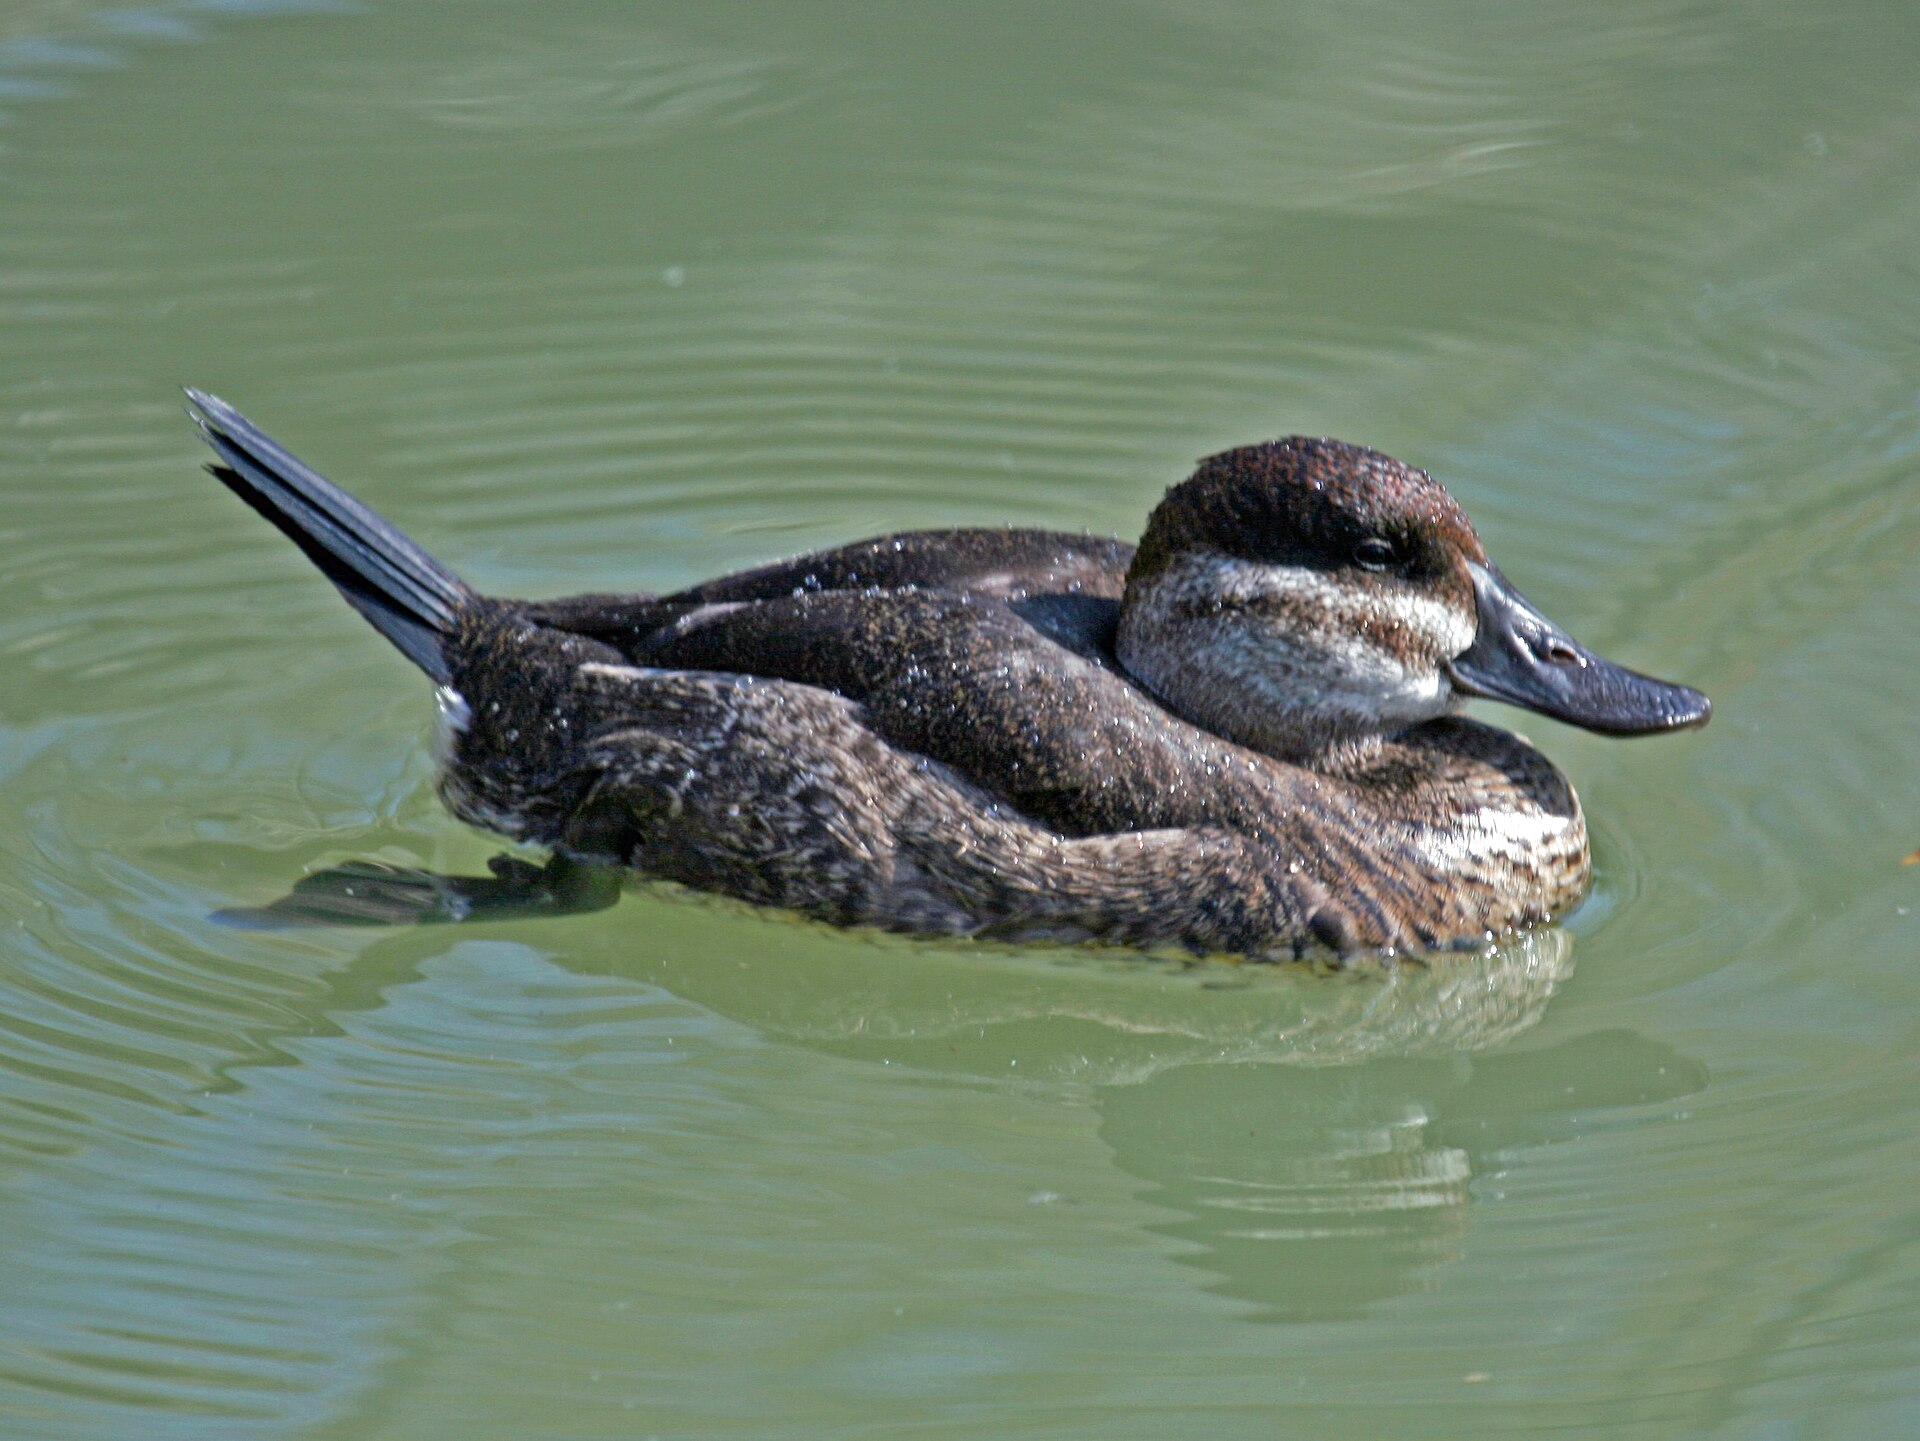
\includegraphics[width=0.7\linewidth, height=3cm, keepaspectratio]{Billeder/Dyr/Fugle/Aender/Dykaender/am_skarveand_hun.jpg}
      \end{minipage}
    }%
    \vspace{0.05em}
    \footnotesize Andrik øverst, and nederst
  \end{columns}
\end{frame}



\section{Gravænder}

\begin{frame}
  \vspace{3em}
  \begin{center}
    {\LARGE \textbf{Gravænder}}
    \vspace{2em}
    \\ Artsbestemmelse og vildtbiologi
\par
{\normalsize }
\vspace{1em}
\par
  \end{center}
\end{frame}

% ========== GRAVAND ==========
\begin{frame}{%
  \begin{minipage}[c]{0.30\textwidth}
    Gravand
  \end{minipage}%
  \hfill
  \begin{minipage}[c]{0.45\textwidth}
    \footnotesize
    \textbf{Jagttid:} Ingen jagttid
  \end{minipage}%
  \hfill
  \begin{minipage}[c]{0.15\textwidth}
    \noindent\raggedleft
    
\includegraphics[width=0.5cm, height=0.5cm, keepaspectratio]{Billeder/Ikoner/star.png}
  \end{minipage}%
}
  \vspace{0.25em}
  \begin{columns}[T]
    % --- Venstre kolonne: Tekst ---
    \column{0.55\textwidth}
    \setlength{\parskip}{0.5em}
    \tiny
    \RaggedRight
    \textbf{\textit{Tadorna tadorna}} – meget stor and som bor i rævegrave (deraf navnet) \par
    \textbf{Udseende:}\\
    \quad – Andrik: Rød, hvid, sort med knop på næbbet \par
    \quad – And: Rød, hvid, sort
    % --- Højre kolonne: To billeder ---
    \column{0.40\textwidth}
    \centering
    \fbox{%
      \begin{minipage}{\linewidth}
        \centering
        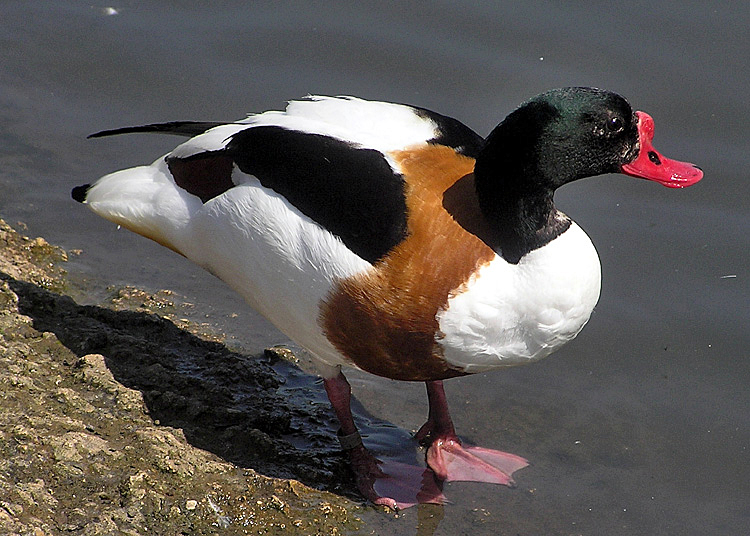
\includegraphics[width=0.7\linewidth, height=3cm, keepaspectratio]{Billeder/Dyr/Fugle/Aender/Gravaender/gravand_han.jpg}\\[0.5em]
        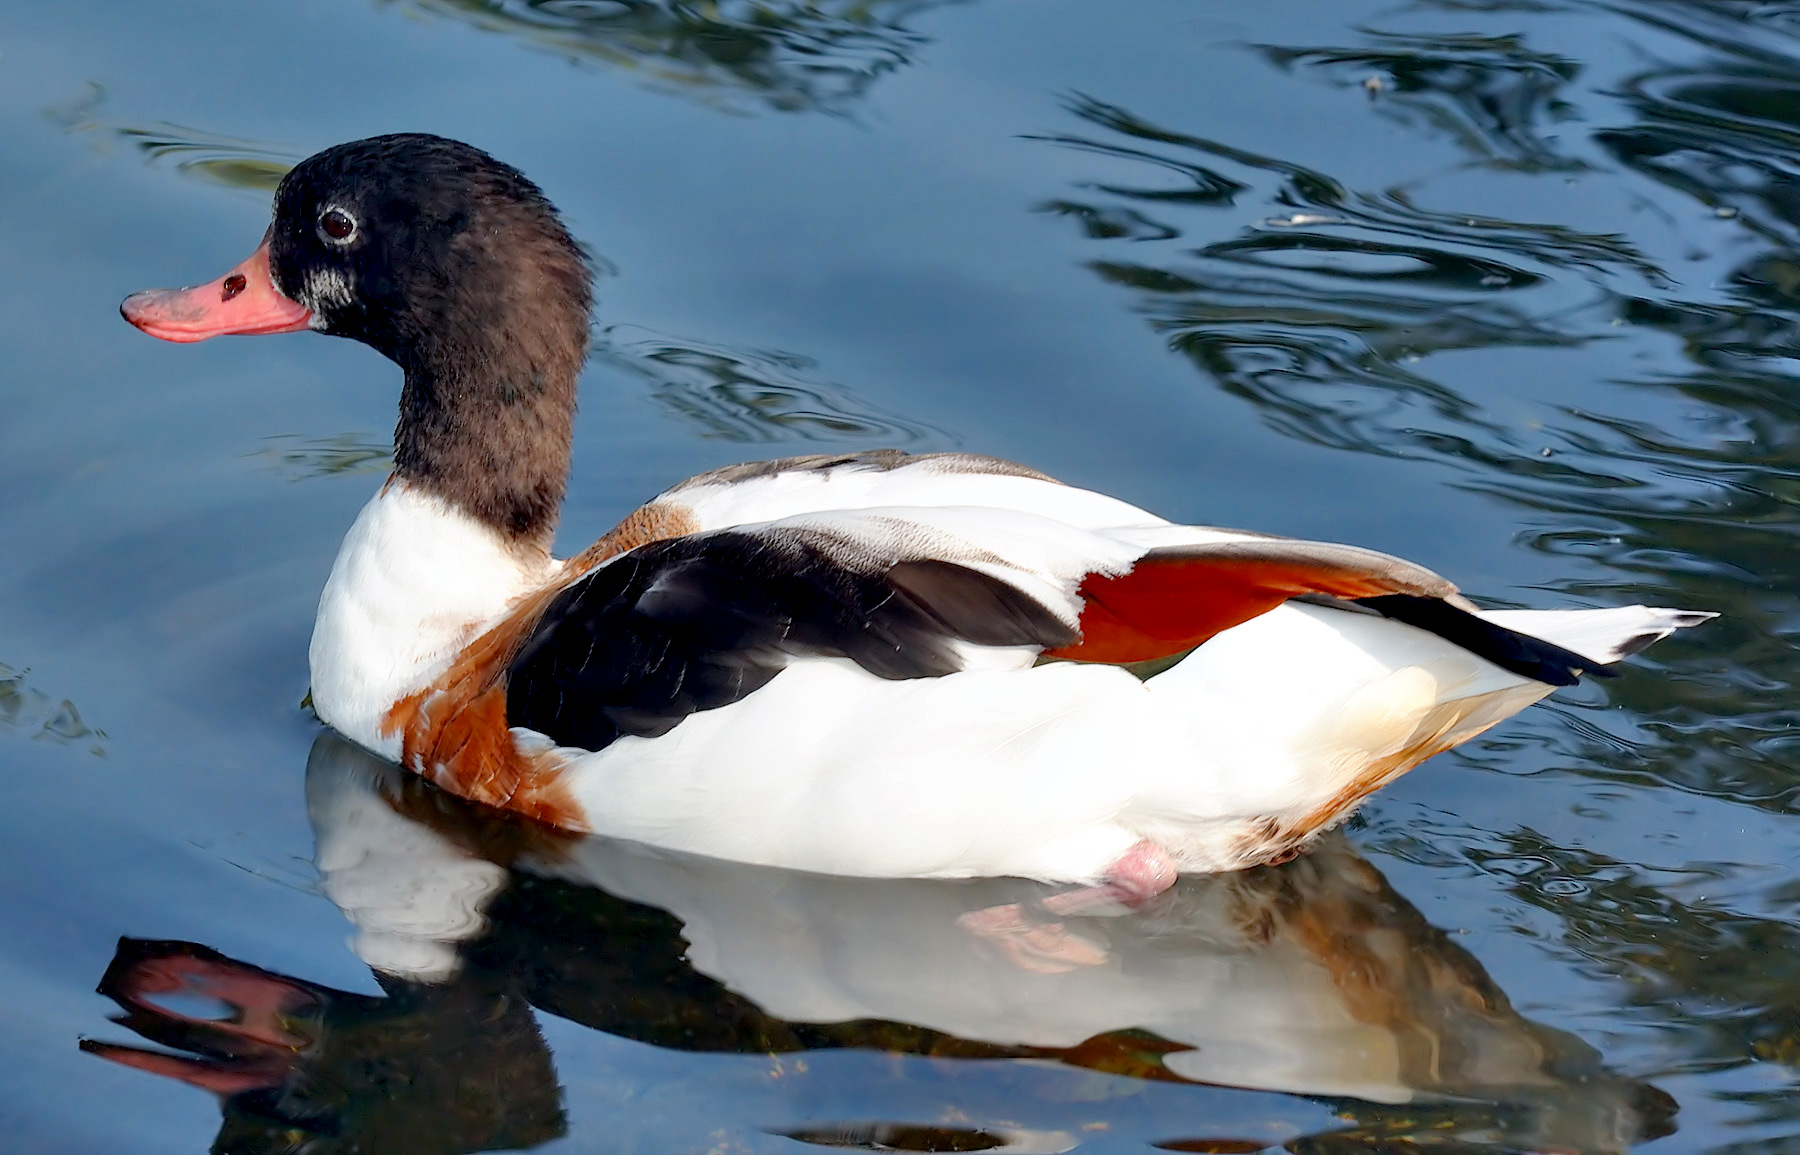
\includegraphics[width=0.7\linewidth, height=3cm, keepaspectratio]{Billeder/Dyr/Fugle/Aender/Gravaender/gravand_hun.jpg}
      \end{minipage}
    }%
    \vspace{0.05em}
    \footnotesize Andrik øverst, and nederst
  \end{columns}
\end{frame}

% ========== NILGÅS ==========
\begin{frame}{%
  \begin{minipage}[c]{0.30\textwidth}
    Nilgås
  \end{minipage}%
  \hfill
  \begin{minipage}[c]{0.45\textwidth}
    \footnotesize
    \textbf{Jagttid:} 1.\ sep. -- 31.\ jan. \\
    \textbf{Regulering:} Uden aftale: Hele året (invasiv)
  \end{minipage}%
  \hfill
  \begin{minipage}[c]{0.15\textwidth}
    \noindent\raggedleft
    
\includegraphics[width=0.5cm, height=0.5cm, keepaspectratio]{Billeder/Ikoner/star.png}
  \end{minipage}%
}
  \vspace{0.25em}
  \begin{columns}[T]
    % --- Venstre kolonne: Tekst ---
    \column{0.55\textwidth}
    \setlength{\parskip}{0.5em}
    \tiny
    \RaggedRight
    \textbf{\textit{Alopochen aegyptiaca}} – stor andelignende fugl som hverken er gås eller and \par
    \textbf{Udseende:}\\
    \quad – Begge: Broget med pletter rundt om øjnene
    % --- Højre kolonne: Ét billede ---
    \column{0.40\textwidth}
    \centering
    \fbox{%
      \begin{minipage}{\linewidth}
        \centering
        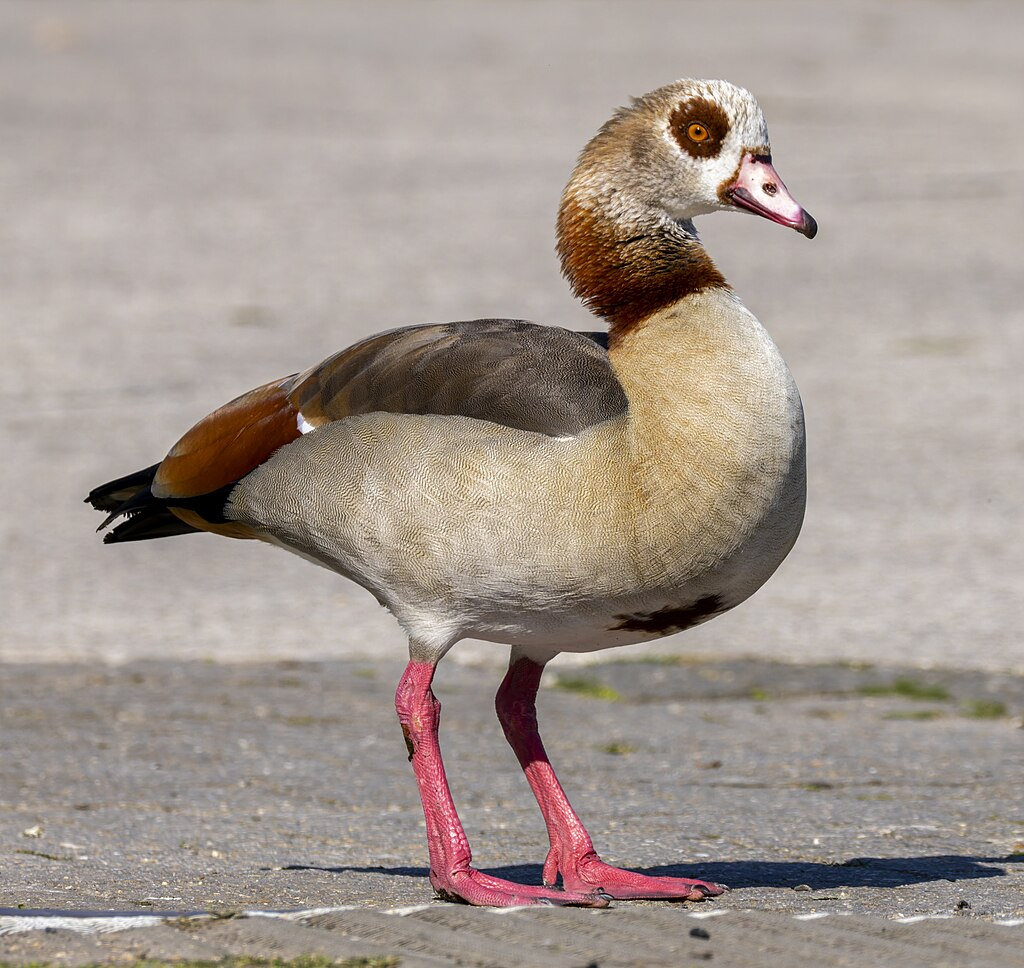
\includegraphics[width=0.85\linewidth, height=5.5cm, keepaspectratio]{Billeder/Dyr/Fugle/Aender/Gravaender/nilgås.jpg}
      \end{minipage}
    }%
  \end{columns}
\end{frame}

\section{Skalleslugere}

\begin{frame}
  \vspace{3em}
  \begin{center}
    {\LARGE \textbf{Skalleslugere}}
    \vspace{2em}
    \\ Artsbestemmelse og vildtbiologi
\par
{\normalsize }
\vspace{1em}
\par
  \end{center}
\end{frame}

\begin{frame}{%
  \begin{minipage}[t]{0.32\textwidth}
    Toppet skallesluger
  \end{minipage}%
  \hfill
  \begin{minipage}[t]{0.36\textwidth}
    \centering
    \footnotesize\textbf{Jagttid:} Ingen jagttid
  \end{minipage}%
  \hfill
  \begin{minipage}[t]{0.15\textwidth}
    \noindent\raggedleft
    
\includegraphics[width=0.5cm, height=0.5cm, keepaspectratio]{Billeder/Ikoner/star.png}%
    \hspace{0.2em}%
    
\includegraphics[width=0.5cm, height=0.5cm, keepaspectratio]{Billeder/Ikoner/star.png}
  \end{minipage}%
} % Ændret: Højre minipage nu med begge ikoner side om side
  \vspace{0.25em}
  \begin{columns}[T]
    % --- Venstre kolonne: Tekst ---
    \column{0.55\textwidth}
    \setlength{\parskip}{0.5em}
    \small
    \RaggedRight\textbf{\textit{Mergus serrator}} – lang slank dykand \par

    \textbf{Udseende:} \\
    \quad – Andrik: metalgrønt hoved, røde øjne, hvid halsring, langt næb \\
    \quad – And: spraglet grå med langt tyndt næb \par

    \textbf{Levesteder:} \\
    \quad – Kyster og fjorde

    \textbf{Føde:} \\
    \quad – Småfisk og krebsdyr \par

    \textbf{Udbredelse:} \\
    \quad – Hele Danmark \par

    \textbf{Træk/standfugl} \\
    \quad – Begge \par

    % --- Højre kolonne: To billeder stablet over hinanden (større størrelse) ---
    \column{0.40\textwidth}
    \centering
    \fbox{%
      \begin{minipage}{\linewidth}
        \centering
        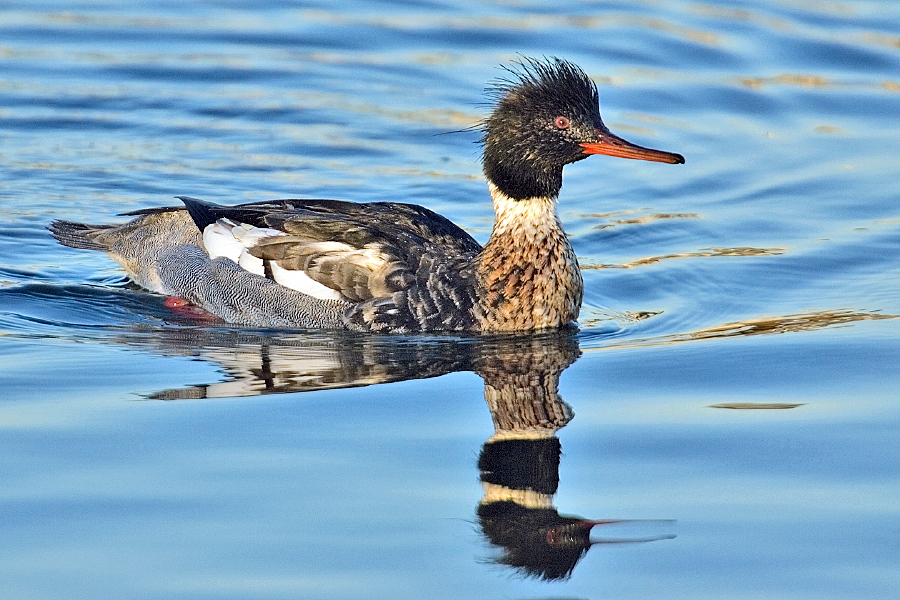
\includegraphics[width=0.8\linewidth, height=3.5cm, keepaspectratio]{Billeder/Dyr/Fugle/Skalleslugere/toppet_skallesluger_han.jpg}\\[0.5em]
        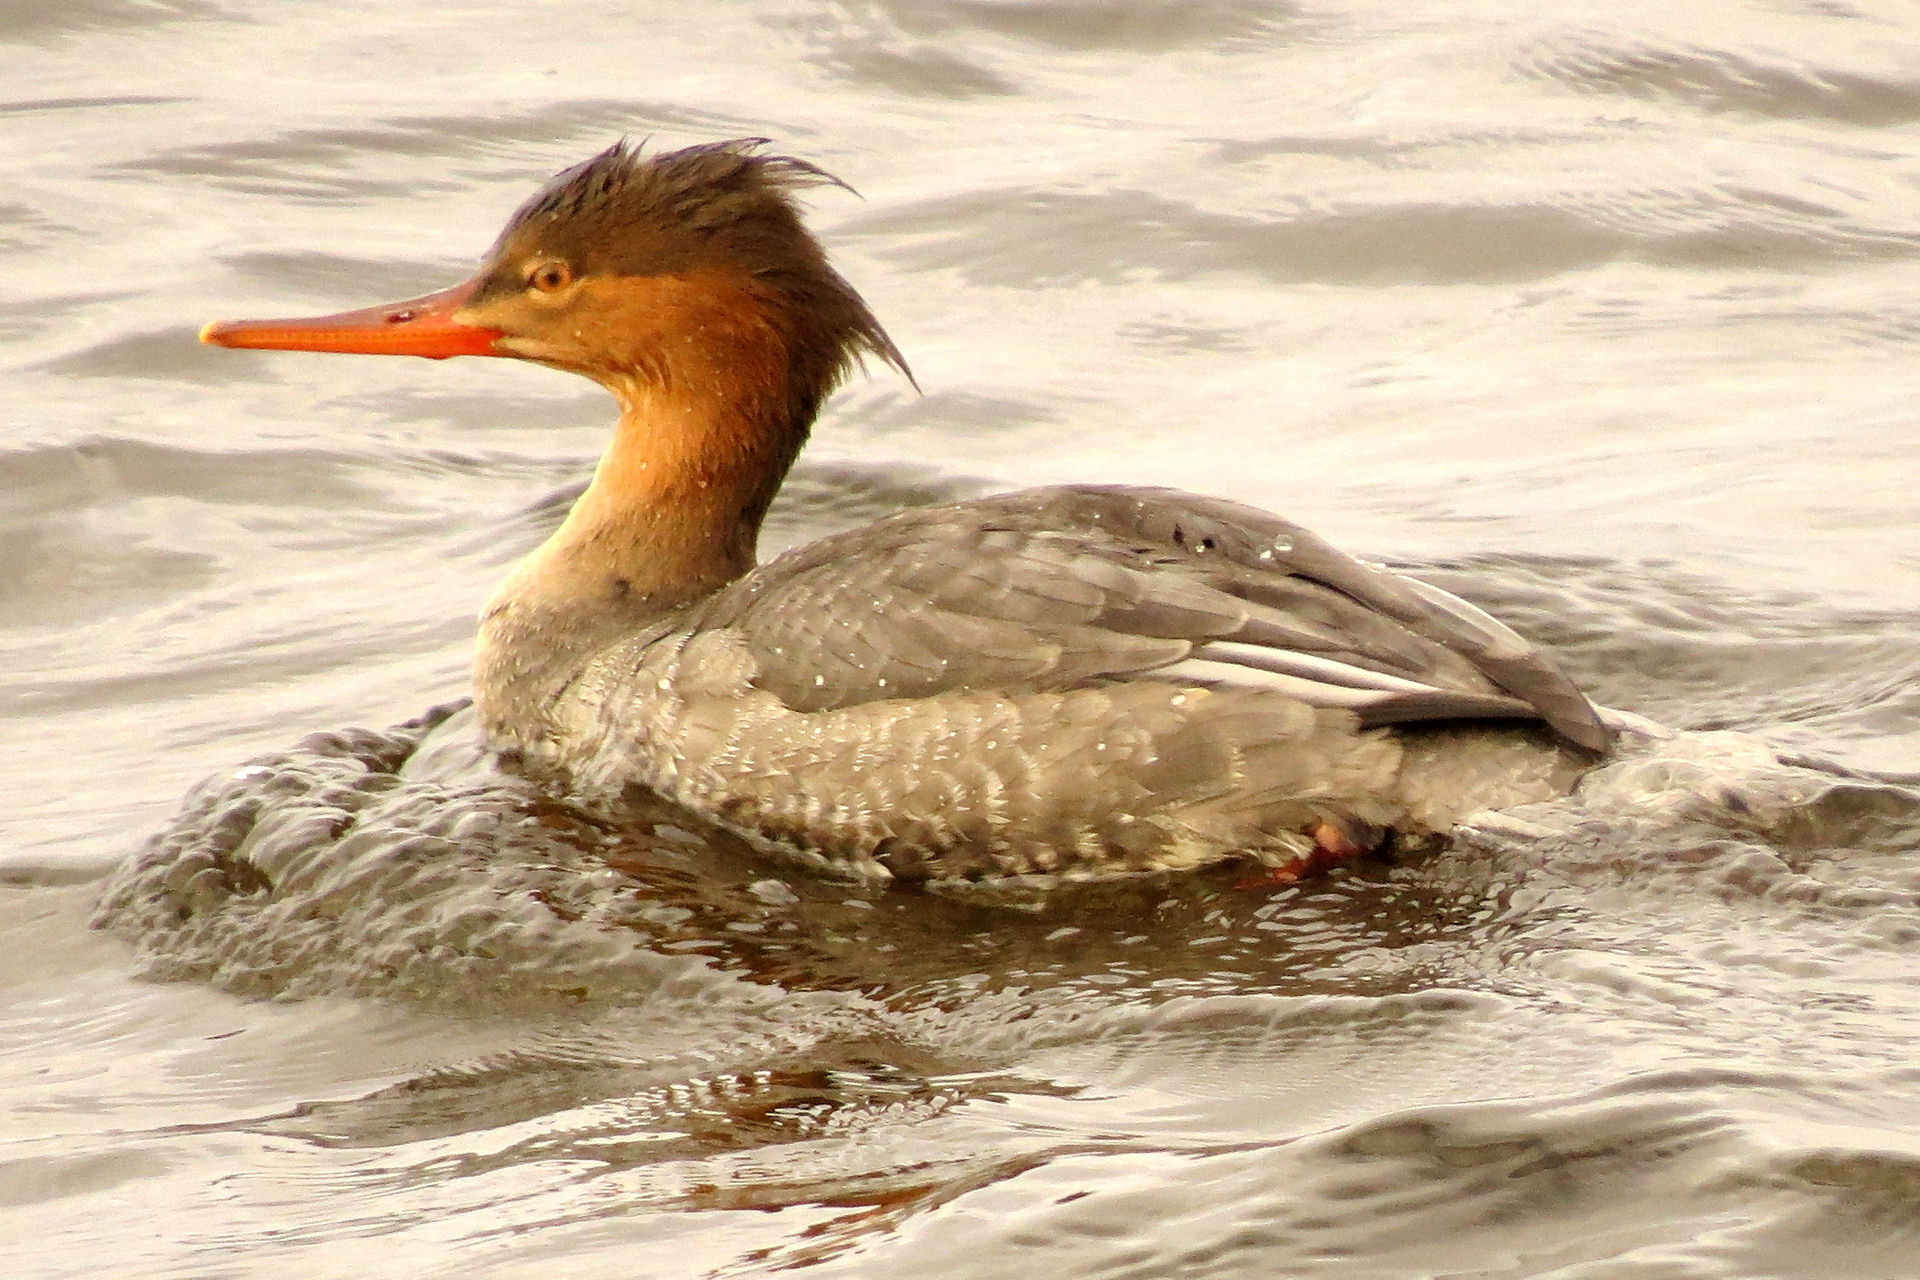
\includegraphics[width=0.8\linewidth, height=3.0cm, keepaspectratio]{Billeder/Dyr/Fugle/Skalleslugere/toppet_skallesluger_hun.jpg}%
      \end{minipage}
    }%
    \vspace{0.05em}
    \footnotesize Andrik øverst, and nederst
  \end{columns}
\end{frame}

\begin{frame}{%
  \begin{minipage}[t]{0.32\textwidth}
    Lille skallesluger
  \end{minipage}%
  \hfill
  \begin{minipage}[t]{0.36\textwidth}
    \centering
    \footnotesize\textbf{Jagttid:} Ingen jagttid
  \end{minipage}%
  \hfill
  \begin{minipage}[t]{0.15\textwidth}
    \noindent\raggedleft
    
\includegraphics[width=0.55cm, height=0.55cm, keepaspectratio]{Billeder/Ikoner/star.png}%
  \end{minipage}%
} 
  \vspace{0.25em}
  \begin{columns}[T]
    % --- Venstre kolonne: Tekst ---
    \column{0.55\textwidth}
    \setlength{\parskip}{0.5em}
    \small
    \RaggedRight\textbf{\textit{Mergellus albellus}} – Mindste skallesluger i Danmark. Anden kan forveksles med andre ænder \par

    \textbf{Udseende:} \\
    \quad – Andrik: hvid med sorte aftegninger \\
    \quad – And: brunt hoved med hvide kinder, kort kraftigt næb \par

    

    % --- Højre kolonne: To billeder stablet over hinanden ---
    \column{0.40\textwidth}
    \centering
    \fbox{%
      \begin{minipage}{\linewidth}
        \centering
        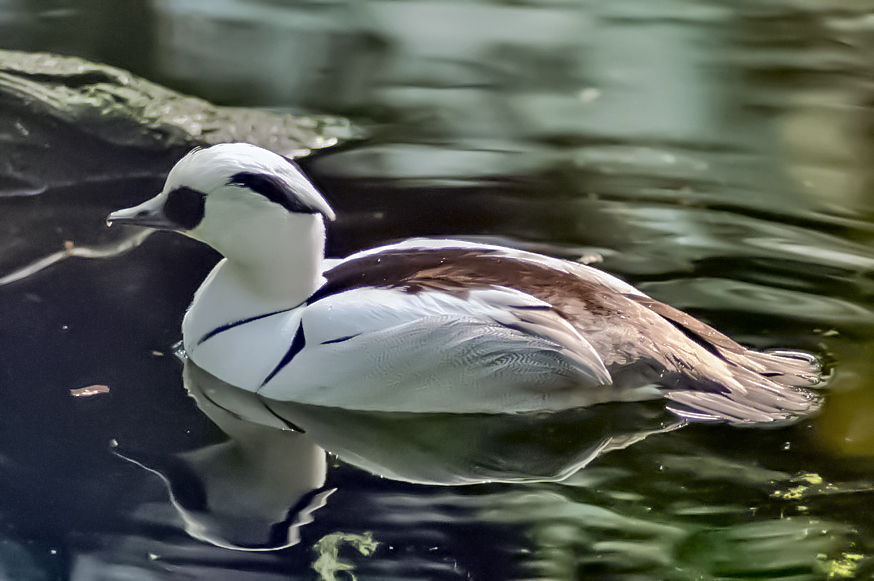
\includegraphics[width=0.8\linewidth, height=3cm, keepaspectratio]{Billeder/Dyr/Fugle/Skalleslugere/lille_skallesluger_han.jpg}\\[0.5em]
        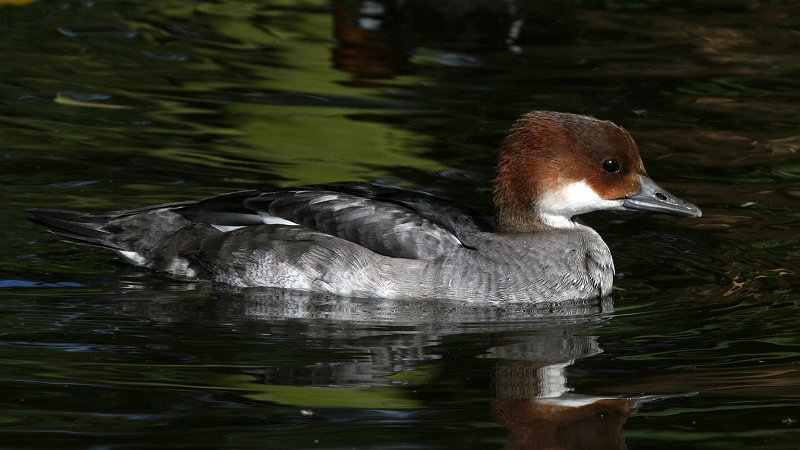
\includegraphics[width=0.8\linewidth, height=3cm, keepaspectratio]{Billeder/Dyr/Fugle/Skalleslugere/lille_skallesluger_hun.jpg}%
      \end{minipage}
    }%
    \vspace{0.05em}
    \footnotesize Andrik øverst, and nederst
  \end{columns}
\end{frame}


\begin{frame}{%
  \begin{minipage}[t]{0.32\textwidth}
    Stor skallesluger
  \end{minipage}%
  \hfill
  \begin{minipage}[t]{0.36\textwidth}
    \centering
    \footnotesize\textbf{Jagttid:} Ingen jagttid
  \end{minipage}%
  \hfill
  \begin{minipage}[t]{0.15\textwidth}
    \noindent\raggedleft
    
\includegraphics[width=0.55cm, height=0.55cm, keepaspectratio]{Billeder/Ikoner/star.png}%
  \end{minipage}%
} 
  \vspace{0.25em}
  \begin{columns}[T]
    % --- Venstre kolonne: Tekst ---
    \column{0.55\textwidth}
    \setlength{\parskip}{0.5em}
    \small
    \RaggedRight\textbf{\textit{Mergus merganser}} – støre skallesluger i Danmark \par

    \textbf{Udseende:} \\
    \quad – Andrik: mørkt hoved, hvid krop, langt rødt næb \\
    \quad – And: pjusket brunt hoved, grå krop \par

    

    % --- Højre kolonne: To billeder stablet over hinanden ---
    \column{0.40\textwidth}
    \centering
    \fbox{%
      \begin{minipage}{\linewidth}
        \centering
        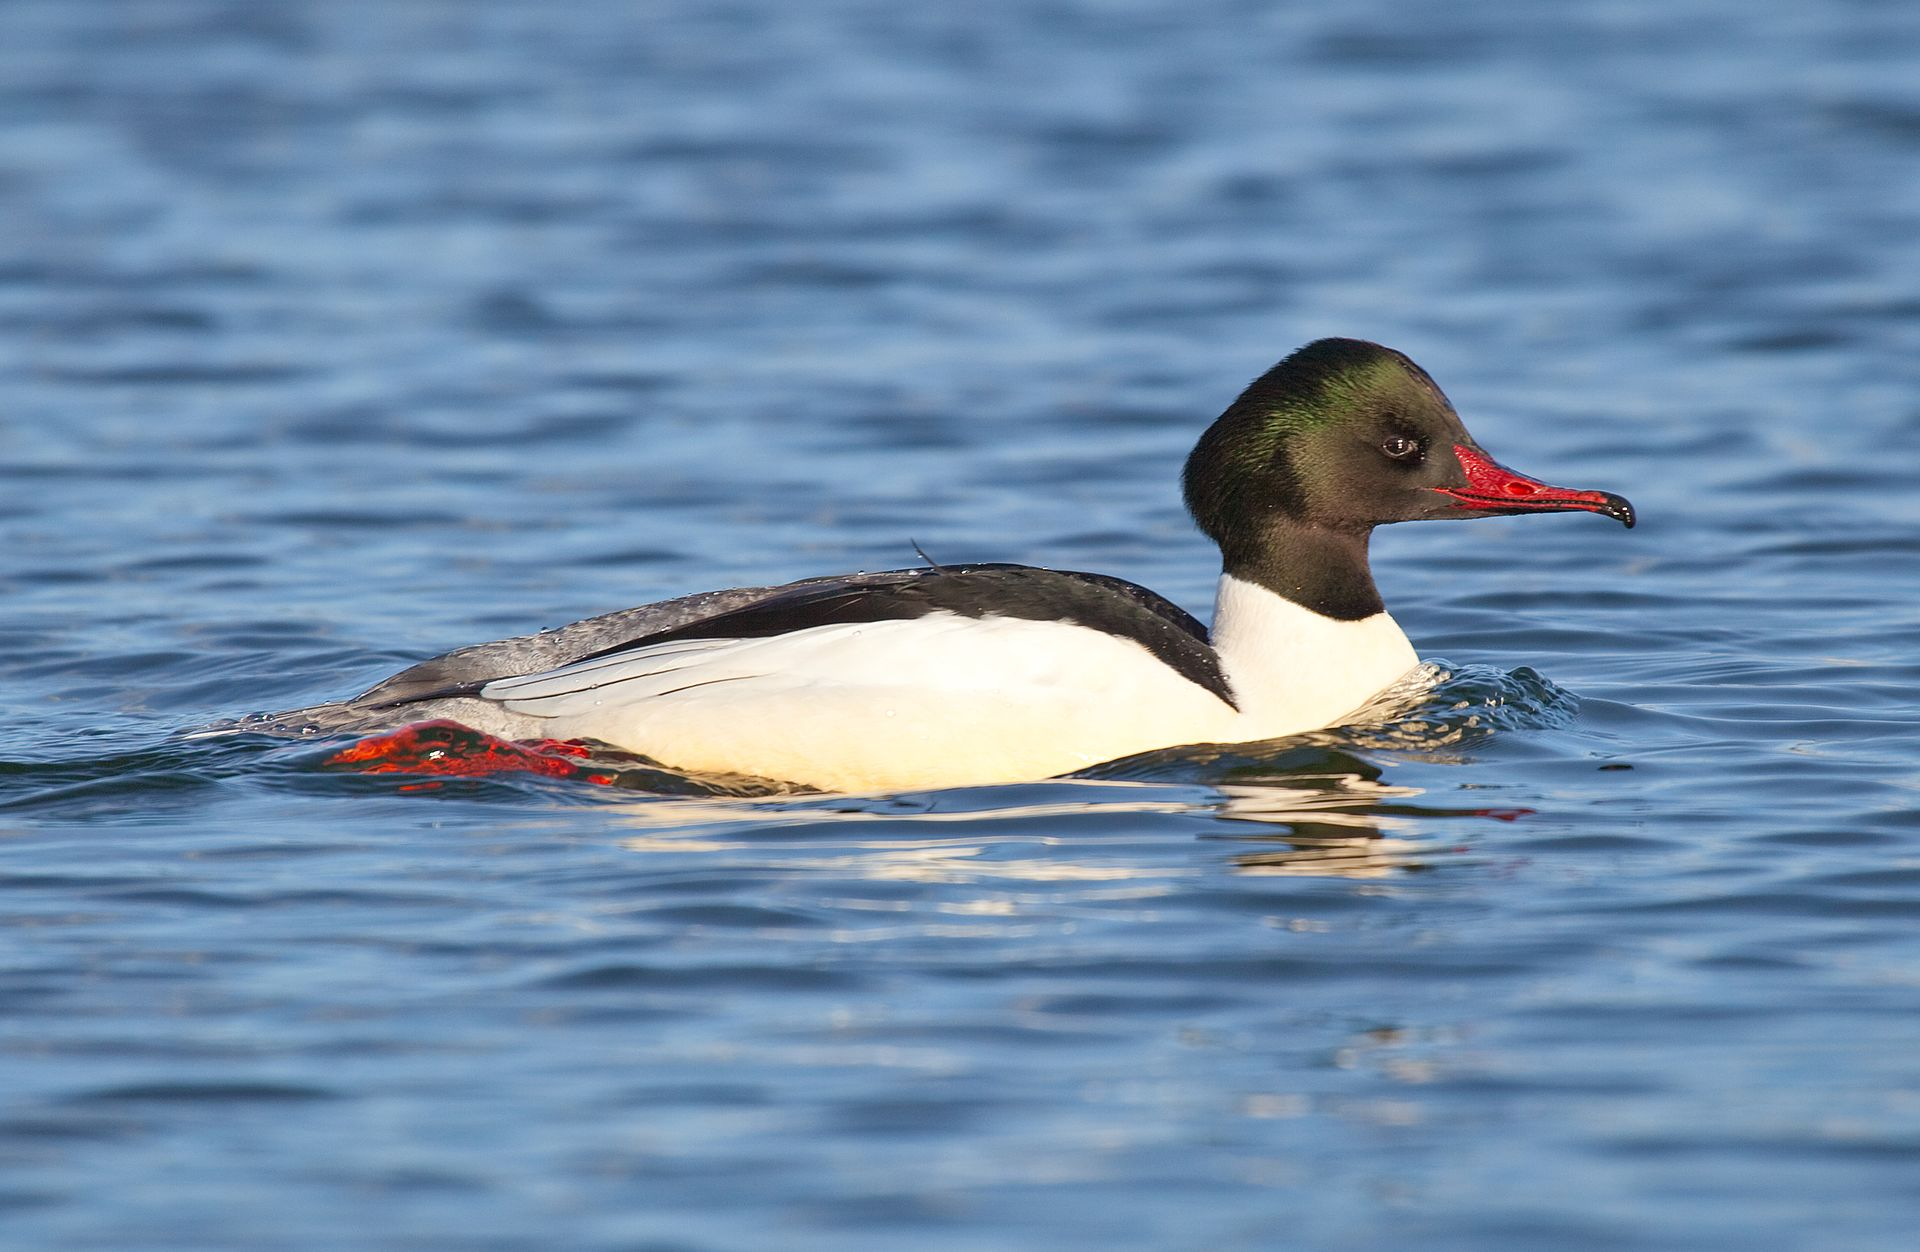
\includegraphics[width=0.8\linewidth, height=3cm, keepaspectratio]{Billeder/Dyr/Fugle/Skalleslugere/stor_skallesluger_han.jpg}\\[0.5em]
        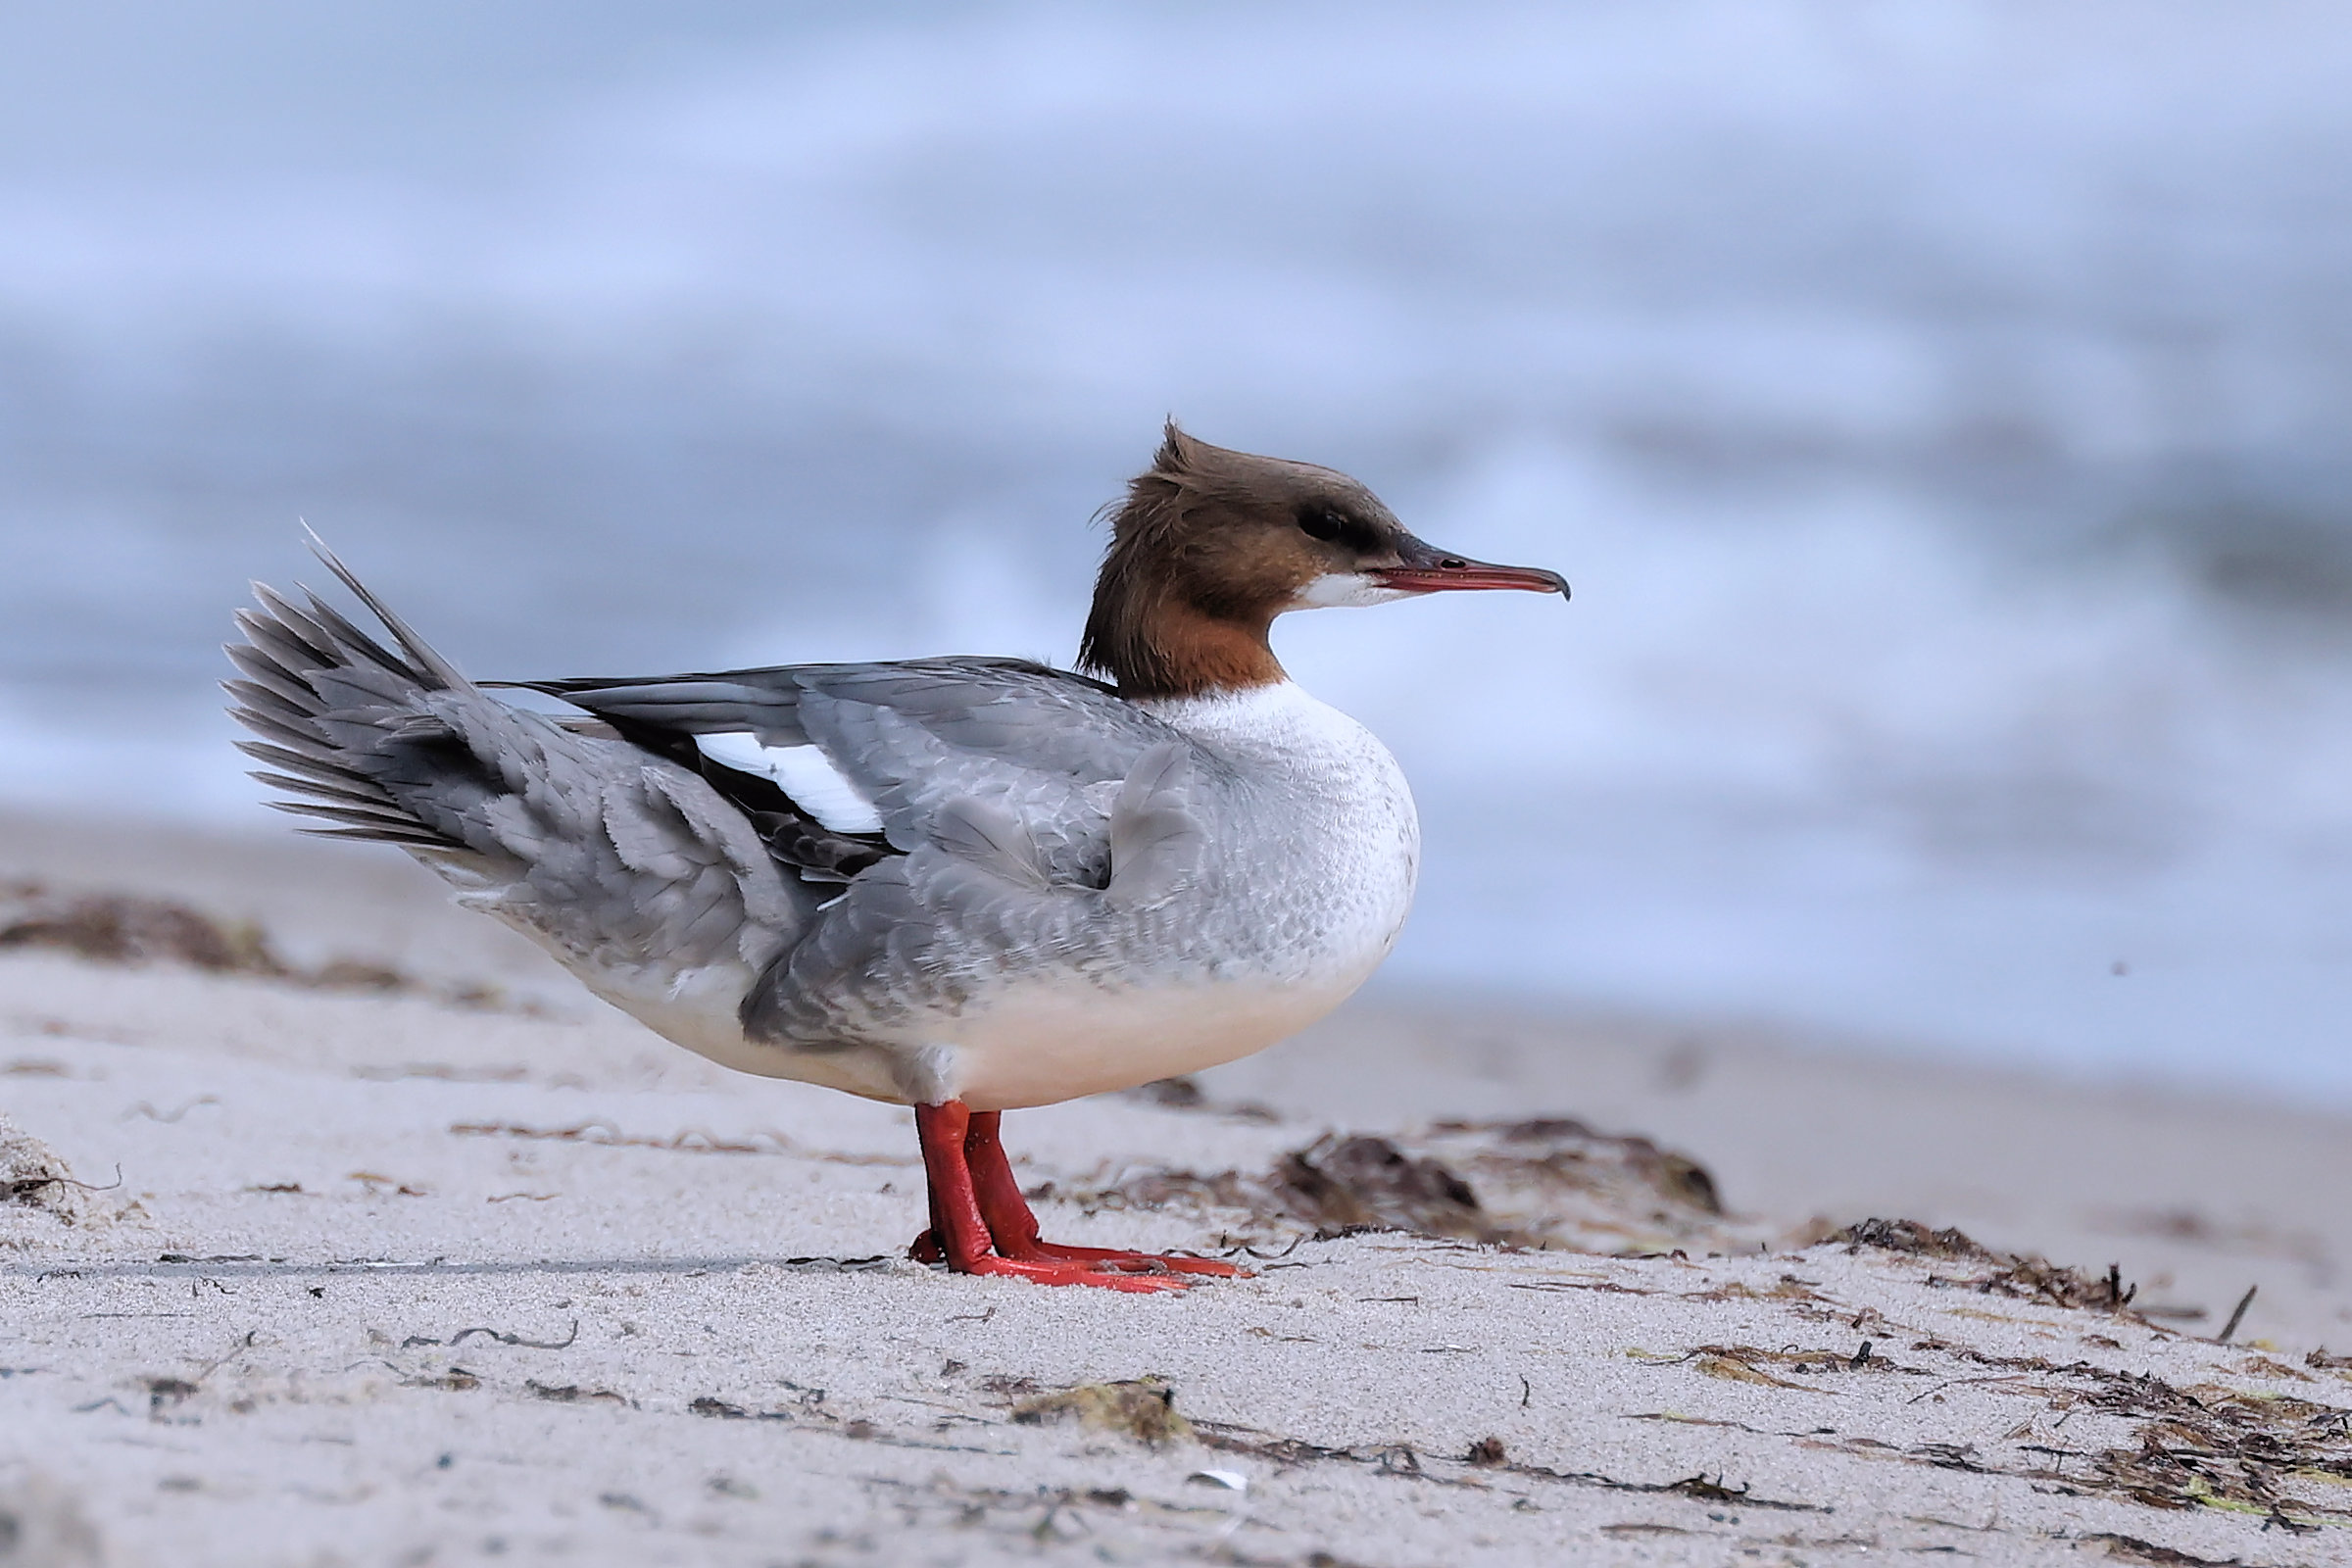
\includegraphics[width=0.8\linewidth, height=3cm, keepaspectratio]{Billeder/Dyr/Fugle/Skalleslugere/stor_skallesluger_hun.jpg}%
      \end{minipage}
    }%
    \vspace{0.05em}
    \footnotesize Andrik øverst, and nederst
  \end{columns}
\end{frame}

\section{Våbenbekendtgørelsen}

\begin{frame}
\vspace{3em}
\begin{center}
{\LARGE \textbf{Bekendtgørelse om våben og ammunition mv.}}
\vspace{2em}
\par
% Våbenbekendtgørelsen
{\normalsize \href{https://www.retsinformation.dk/eli/lta/2021/2531}{BEK nr 2531 af 20/12/2021}}
\vspace{1em}
\par

\end{center}
\end{frame}

\begin{frame}{Adgang til Våben: Jagttegn og Tilladelser}

\vspace{1em}

\begin{columns}[c] % c = center vertically

\column{0.05\textwidth} % Venstre margin

\column{0.7\textwidth} % Midten: Bullets

\small

\raggedright

\begin{itemize}

\itemsep0.6em % Justér afstand mellem bullets

\item Et jagttegn udstedes kun med \textbf{samtykke fra Politiet} (vurdering af vandel/egnethed, jf. § 6).

\item Du skal være fyldt \textbf{18 år} for selv at kunne \structure{erhverve} og \structure{besidde} skydevåben.

\item Våben må kun håndteres af personer, der kan fremvise \textbf{gyldigt jagttegn} eller \structure{våbentilladelse} (§ 20).

\item Du må bruge haglgevær under \structure{jagtprøven} og til instruktion, da kursuslærere må overlade våben til dig (§ 21).

\item \textbf{Ungjægerordningen}: Er du under 18 år, skal du jage \textbf{i følge med} en myndig jæger (over 18 år).

\end{itemize}

\column{0.25\textwidth} % Højre: Ikon

\centering

\vspace{0pt}


\includegraphics[width=0.9\linewidth]{Billeder/Redskaber/jagttegn_billede.jpg} % Antager et ikon, der passer til 'Tilladelse' (evt. et jagttegn)

\end{columns}

\end{frame}
\begin{frame}{Opbevaring af våben og ammunition § 24}

\vspace{1em}

\begin{columns}[c] % c = center vertically

\column{0.05\textwidth} % Venstre margin (kan fjernes eller justeres)



\column{0.7\textwidth} % Midten: Bullets

\small

\raggedright



\begin{itemize}

\itemsep0.6em % Justér afstand mellem bullets

\item Våben og ammunition skal opbevares forsvarligt og \textbf{utilgængeligt} for uvedkommende.

\item Skabe under \textbf{1.000 kg} skal være fastboltet til gulv/væg.

\item Nøgler til skabet skal opbevares separat og utilgængeligt.

\item Der sondres mellem to typer af våbenskabe, som styres af antallet af våben, der skal opbevares.

\item Max 25 regulære våben, hvor max 10 våben må være særligt farlige våben \textbf{kræver} (min. EN 1143-1 \textbf{Grade 0}).

\item Flere end 25 regulære våben og/eller 10 særligt farlige våben \textbf{kræver} (min. EN 1143-1 \textbf{Grade 1}).

\item Ammunition må opbevares ved siden af, men ikke i våbnet.

\end{itemize}



\column{0.25\textwidth} % Højre: Ikon (størrelsen tilpasses her)

\centering

\vspace{0pt} % hjælper med vertikal centring i nogle temaer

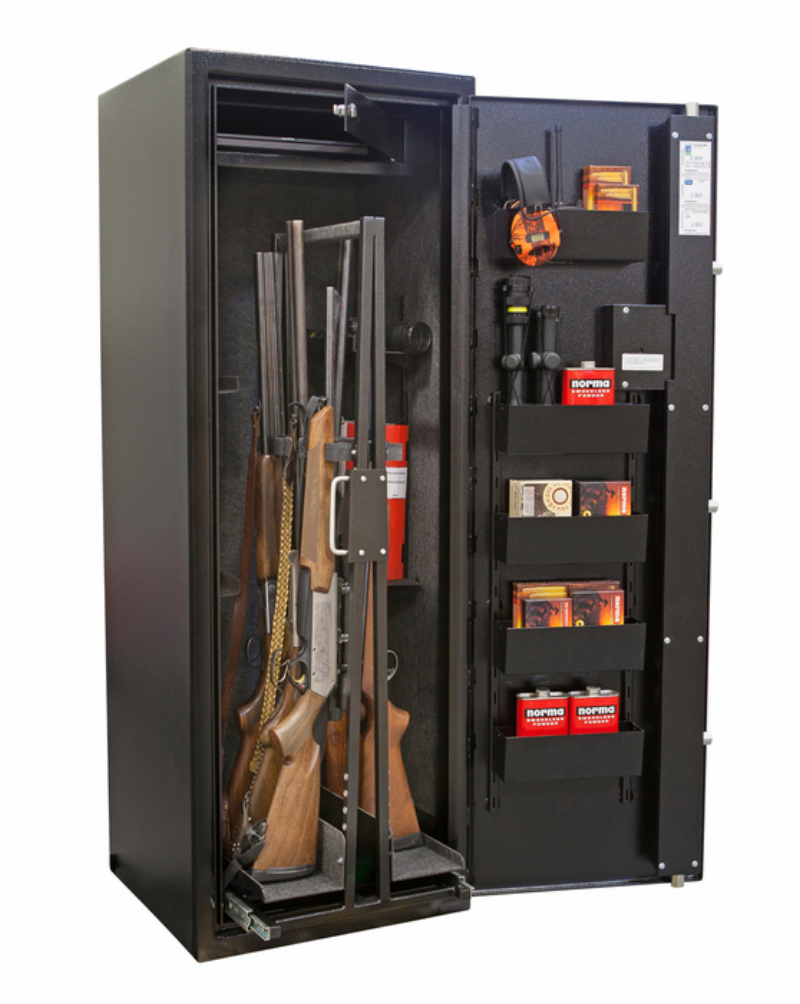
\includegraphics[width=0.8\linewidth]{Billeder/Redskaber/vaabenskab.png}



\end{columns}

\end{frame}
\begin{frame}{Særligt farlige våben og sikringskrav}

\begin{itemize}
    \item \textbf{Særligt farlige våben} (defineret i bekendtgørelsen):
    \begin{itemize}
        \item Pistoler (inkl. enkeltskud, halvautomatiske, revolvere – undtagen forladevåben)
        \item Fuld- og halvautomatiske våben (halvautomatisk haglgevær)
        \item Glatløbede haglgeværer med pibelængde under 55 cm
    \end{itemize}
    \vspace{1em}
    \item \textbf{Vigtigt at huske}:
    \begin{itemize}
        \item Det samlede antal våben på adressen afgør sikringskravet – også selvom våbnene opbevares i flere skabe
        \item Sikringsniveauet er strengere for særligt farlige våben, da de anses for en større risiko end et højere antal almindelige våben
    \end{itemize}
\end{itemize}

\end{frame}
\begin{frame}{Overdragelse og Overladelse af Våben (§ 20)}

\vspace{1em}

\begin{columns}[c] % c = center vertically

\column{0.05\textwidth} % Venstre margin

\column{0.7\textwidth} % Midten: Bullets

\small

\raggedright

\begin{itemize}

\itemsep0.3em % Justér afstand mellem bullets

\item \textbf{Hovedregel:} Våben må kun overdrages eller overlades til personer, der kan fremvise \structure{fornøden våbentilladelse}.

\item \textbf{Forskel riffel og haglvåben:} Haglvåben kan overlades til en anden person med jagttegn. Riffel må kun overdrages til person med våbentilladelse til pågældende våben.

\item \textbf{Identifikation:} Den, der modtager våbnet, skal fremvise \structure{original billedlegitimation} for at bevise, at tilladelsen tilhører vedkommende.

\item \textbf{Udlåners ansvar:} Den, der låner våbnet ud, har pligt til at kontrollere \structure{både tilladelse og legitimation}.

\item \textbf{Ungjægere:} Glatløbede haglgeværer må overlades til kursister/aspiranter af \textbf{godkendte lærere/prøvesagkyndige} i forbindelse med instruktion og prøve (§ 21).

\end{itemize}

\column{0.25\textwidth} % Højre: Ikon

\centering

\vspace{0pt}

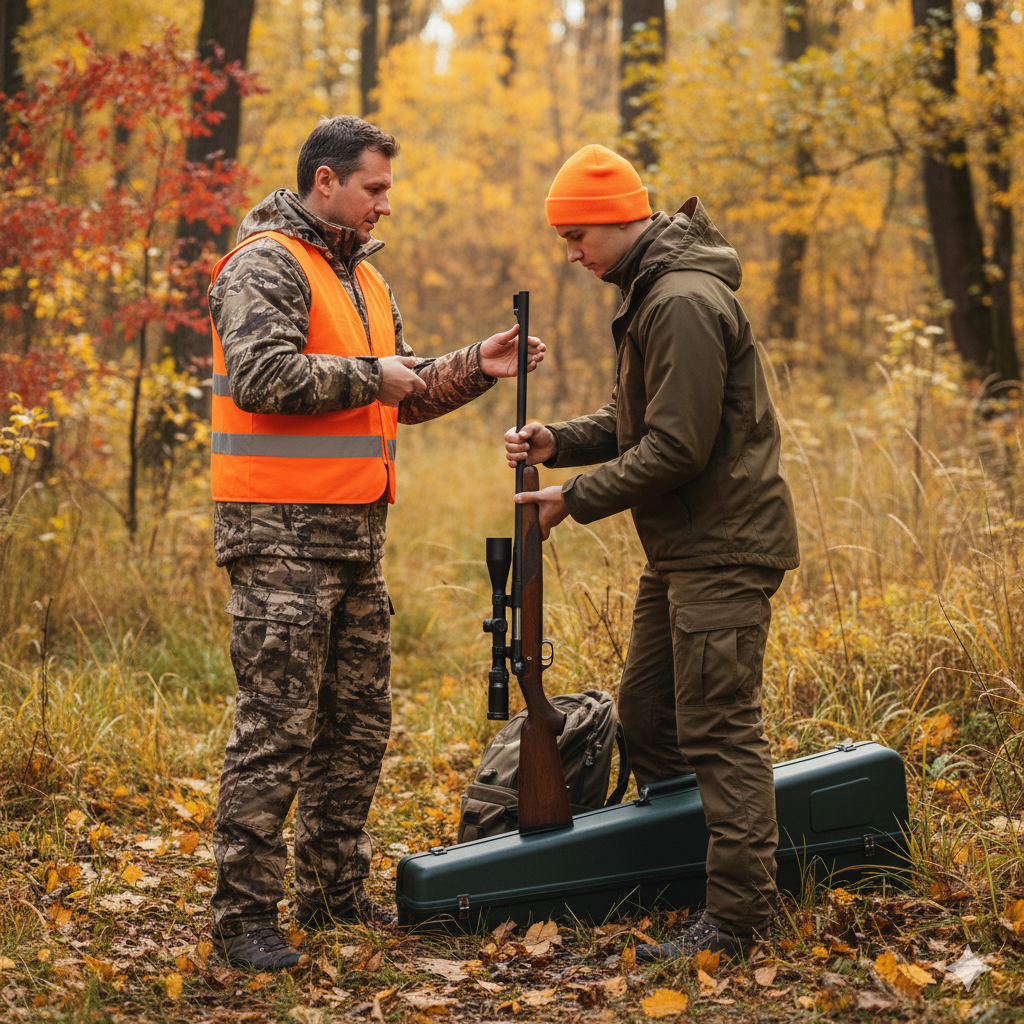
\includegraphics[width=0.9\linewidth]{Billeder/Redskaber/overdragelse.png} % Forslag til et ikon, der symboliserer overladelse/aftale

\end{columns}

\end{frame}
\begin{frame}{Transport af Skydevåben (§ 11)}

\vspace{1em}

\begin{columns}[c] % c = center vertically

\column{0.05\textwidth} % Venstre margin

\column{0.7\textwidth} % Midten: Bullets

\small

\raggedright

\begin{itemize}

\itemsep0.6em % Justér afstand mellem bullets

\item \textbf{Formål:} Transport må kun ske i forbindelse med anerkendelsesværdige formål (f.eks. til/fra \structure{opbevaring, anvendelsessted, køb/salg eller reparation}).

\item \textbf{Forsvarlighed:} Våben skal transporteres \textbf{forsvarligt} (f.eks. under konstant tilsyn eller tildækket i aflåst transportmiddel).

\item \textbf{Indpakning:} Skydevåben skal være \structure{indpakket i lukket etui eller lignende} (f.eks. våbenkuffert).

\item \textbf{Ammunition:} Skydevåben må \textbf{IKKE indeholde ammunition} under transport uden for anvendelsesområdet (jagt/skydebane).

\item \textbf{Bæring:} Våben må \textbf{IKKE} transporteres i side- eller skulderhylstre på kroppen.

\end{itemize}

\column{0.25\textwidth} % Højre: Ikon

\centering

\vspace{0pt}

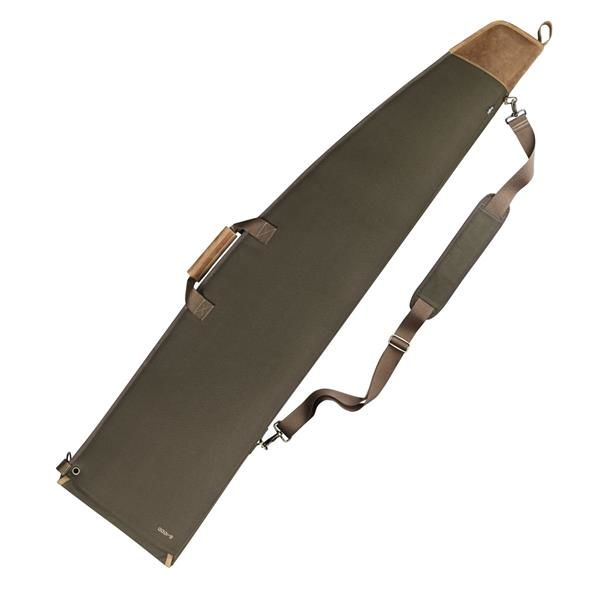
\includegraphics[width=0.9\linewidth]{Billeder/Redskaber/futeral.jpg} % Forslag til et ikon, der symboliserer transport/bil

\end{columns}

\end{frame}

\section{Cirkulære om våben og ammunition m.v.}

\begin{frame}
  \vspace{3em}
  \begin{center}
    {\LARGE \textbf{Cirkulære om våben og ammunition m.v.}} \\
    \vspace{1em}
    CIR1H nr 10066 af 29/10/2025, § 16
  \end{center}
\end{frame}

\begin{frame}{\S\ 16, Personer under 18 år}
\begin{itemize}
    \item Tilladelse kan gives til personer under 18 år, hvis de:
    \begin{itemize}
        \item er medlem af skytte- eller jagtforening og fyldt 16 år, eller
        \item har jagttegn
    \end{itemize}
    \item Personer fyldt 16 år kan desuden få tilladelse til luft-/fjedervåben ($\leq$ 4,5 mm)
    \item Tilladelse til foreningsmedlemmer gælder kun våben, der anvendes i foreningen
    \item Tilladelse kræver skriftligt samtykke fra forældremyndighedsindehavere, som også påtager sig opbevaringsansvar
    \item Politiet skal sikre, at forældre er bekendt med rettigheder/pligter og opfylder opbevaringskrav (\S\ 48 i våbenbekendtgørelsen)
\end{itemize}
\end{frame}

\section{Repetition Teori 1}

\begin{frame}
  \vspace{3em}
  \begin{center}
    {\LARGE \textbf{Repetition: Teori 1 (Kahoot)}}
  \end{center}
\end{frame}

% ========== TITEL: GÆS ==========
\begin{frame}
  \vspace{1.5em}
  \begin{center}
    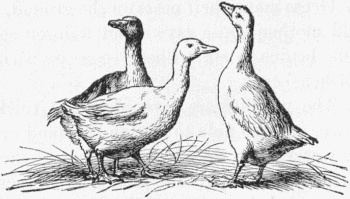
\includegraphics[width=12cm, height=4cm, keepaspectratio]{Billeder/Dyr/Fugle/Gaes/gæs.jpg}\\[1.2em]
    {\LARGE \textbf{Gæs}}\\[0.6em]
    
    Artsbestemmelse \&  vildtbiologi \\[0.9em]
    {\tiny\color{gray}
    CC BY 4.0 – kan frit anvendes, også kommercielt. Rettighederne må ikke skærpes.\\[0.05em]
    Udviklet af Aleksander Sønder, OSJAGTTEGN.DK}
  \end{center}
\end{frame}

% ========== GRÅGÅS ==========
\begin{frame}{%
  \begin{minipage}[c]{0.30\textwidth}
    Grågås
  \end{minipage}%
  \hfill
  \begin{minipage}[c]{0.45\textwidth}
    \footnotesize
    \textbf{Jagttid:} 1.\ sep.--31.\ jan. samt 1.\--31.\ aug.* \\
    \textbf{Regulering:} Efter aftale: 1.\--31.\ jul. \& 1.\--29.\ jan.
  \end{minipage}%
  \hfill
  \begin{minipage}[c]{0.15\textwidth}
    \noindent\raggedleft
    
\includegraphics[width=0.5cm, height=0.5cm, keepaspectratio]{Billeder/Ikoner/star.png}%
    \hspace{0.2em}%
    
\includegraphics[width=0.5cm, height=0.5cm, keepaspectratio]{Billeder/Ikoner/star.png}%
    \hspace{0.2em}%
    
\includegraphics[width=0.5cm, height=0.5cm, keepaspectratio]{Billeder/Ikoner/star.png}
  \end{minipage}%
}
  \vspace{0.25em}
  \begin{columns}[T]
    % --- Venstre kolonne: Tekst ---
    \column{0.45\textwidth}
    \setlength{\parskip}{0.5em}
    \tiny
    \RaggedRight
    \textbf{\textit{Anser anser}} – største af de grå gæs \par
    \textbf{Udseende:}\\
    \quad – Kødfarvede ben \\
    \quad – Kraftig hals \\
    \quad – Orangerødt næb \par
    \textbf{Levesteder:} Nær vådområder og på marker. \par
    \textbf{Føde:} Planteføde. \par
    \textbf{Udbredelse:} Hele Danmark. \par
    \textbf{Træk/standfugl:} Begge \par
    \textbf{Forplantning:}\\
    \quad – \textbf{Yngleforhold:} Yngler i hele Danmark \\
    \quad – \textbf{Kønsmoden:} Ca. 3 år \\
    \quad – \textbf{Mono/polygam:} Monogam \\
    \quad – \textbf{Bestandsomsætning:} Langsom \\
    \quad – \textbf{Kuld:} 4–6 æg
    \par
    \textbf{* Jagttid 1. - 31. august:} \\
    \quad – \textbf{Krav} På arealer i omdrift (aktive marker/landbrug) med minimumsafstand på 300m til ferske vandre større end 3ha
    % --- Højre kolonne: Større billede ---
    \column{0.52\textwidth}
    \centering
    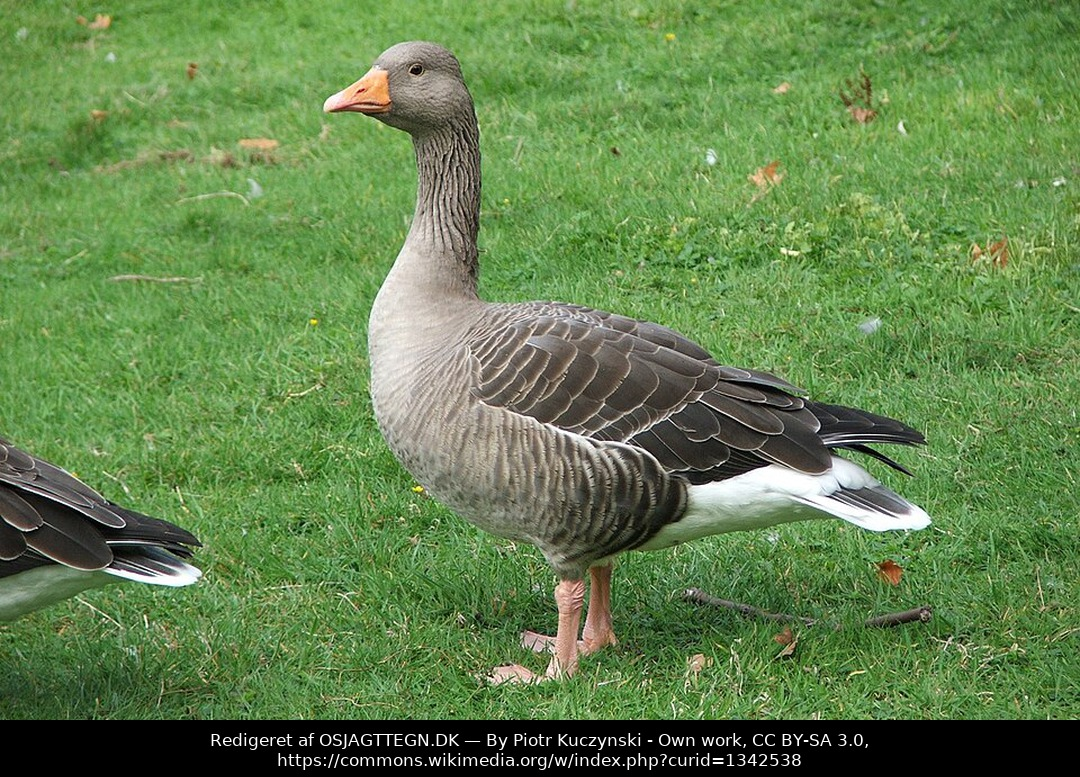
\includegraphics[width=\linewidth, height=7.2cm, keepaspectratio]{Billeder/Dyr/Fugle/Gaes/grågås.jpg}
  \end{columns}
\end{frame}
% ========== KNORTEGÅS ==========
\begin{frame}{%
  \begin{minipage}[c]{0.30\textwidth}
    Knortegås
  \end{minipage}%
  \hfill
  \begin{minipage}[c]{0.45\textwidth}
    \footnotesize
    \textbf{Jagttid:} Ingen jagttid
  \end{minipage}%
  \hfill
  \begin{minipage}[c]{0.15\textwidth}
    \noindent\raggedleft
    
\includegraphics[width=0.5cm, height=0.5cm, keepaspectratio]{Billeder/Ikoner/star.png}%
    \hspace{0.2em}%
    
\includegraphics[width=0.5cm, height=0.5cm, keepaspectratio]{Billeder/Ikoner/star.png}
  \end{minipage}%
}
  \vspace{0.25em}
  \begin{columns}[T]
    % --- Venstre kolonne: Tekst ---
    \column{0.45\textwidth}
    \setlength{\parskip}{0.5em}
    \tiny
    \RaggedRight
    \textbf{\textit{Branta bernicla}} – lille rajgås hvor navnet refererer til deres knurrende kald \par
    \textbf{Udseende:}\\
    \quad – Mørk med hvid halsring \par
    \textbf{Levesteder:} Kyster og fjorde. \par
    \textbf{Føde:} Ålegræs. \par
    \textbf{Udbredelse:} Overvintrer langs kysterne i Danmark. \par
    \textbf{Træk/standfugl:} Trækfugl
    % --- Højre kolonne: Større billede ---
    \column{0.52\textwidth}
    \centering
    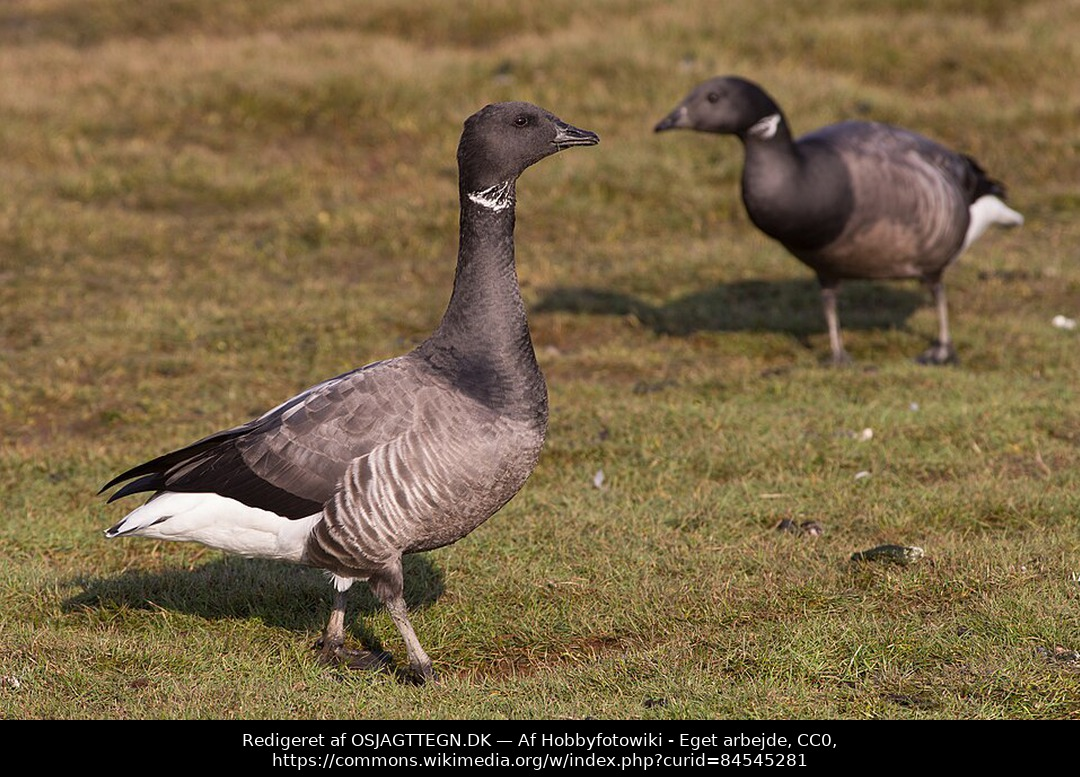
\includegraphics[width=\linewidth, height=7.2cm, keepaspectratio]{Billeder/Dyr/Fugle/Gaes/knortegås.jpg}
  \end{columns}
\end{frame}
% ========== KORTNÆBBET GÅS ==========
\begin{frame}{%
  \begin{minipage}[c]{0.30\textwidth}
    Kortnæbbet gås
  \end{minipage}%
  \hfill
  \begin{minipage}[c]{0.45\textwidth}
    \footnotesize
    \textbf{Jagttid:} 1.\ september -- 31.\ januar
  \end{minipage}%
  \hfill
  \begin{minipage}[c]{0.15\textwidth}
    \noindent\raggedleft
    
\includegraphics[width=0.5cm, height=0.5cm, keepaspectratio]{Billeder/Ikoner/star.png}%
    \hspace{0.2em}%
    
\includegraphics[width=0.5cm, height=0.5cm, keepaspectratio]{Billeder/Ikoner/star.png}
  \end{minipage}%
}
  \vspace{0.25em}
  \begin{columns}[T]
    % --- Venstre kolonne: Tekst ---
    \column{0.45\textwidth}
    \setlength{\parskip}{0.5em}
    \tiny
    \RaggedRight
    \textbf{\textit{Anser brachyrhynchus}} – kendes på det korte næb, men forveksles let med de øvrige grå gæs \par
    \textbf{Udseende:}\\
    \quad – Kort kraftigt lyserødt næb, lyserøde ben \par
    \textbf{Levesteder:} Vådområder og landbrugsarealer. \par
    \textbf{Føde:} Planteføde. \par
    \textbf{Udbredelse:} Langs vestkysten som trækfugl. \par
    \textbf{Træk/standfugl:} Trækfugl
    % --- Højre kolonne: Større billede ---
    \column{0.52\textwidth}
    \centering
    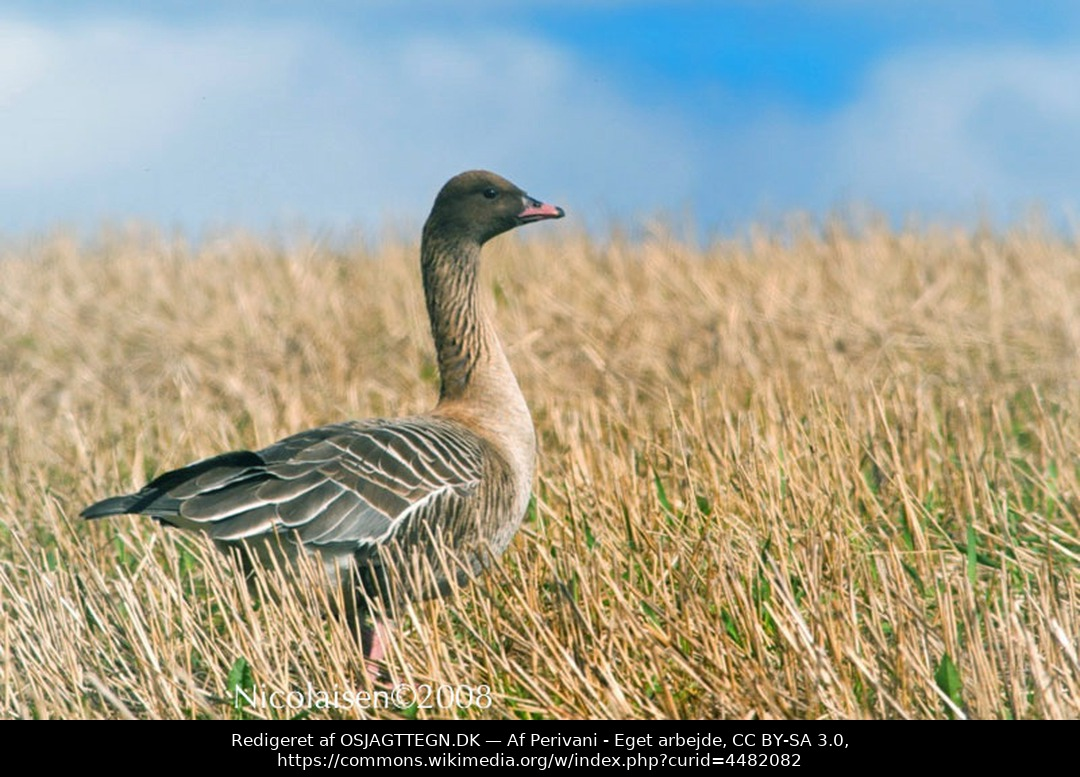
\includegraphics[width=\linewidth, height=7.2cm, keepaspectratio]{Billeder/Dyr/Fugle/Gaes/kortnæbbet_gås.jpg}
  \end{columns}
\end{frame}
% ========== SÆDGÅS ==========
\begin{frame}{%
  \begin{minipage}[c]{0.30\textwidth}
    Sædgås
  \end{minipage}%
  \hfill
  \begin{minipage}[c]{0.45\textwidth}
    \footnotesize
    \textbf{Jagttid:} Ingen jagttid
  \end{minipage}%
  \hfill
  \begin{minipage}[c]{0.15\textwidth}
    \noindent\raggedleft
    
\includegraphics[width=0.5cm, height=0.5cm, keepaspectratio]{Billeder/Ikoner/star.png}
  \end{minipage}%
}
  \vspace{0.25em}
  \begin{columns}[T]
    % --- Venstre kolonne: Tekst ---
    \column{0.45\textwidth}
    \setlength{\parskip}{0.5em}
    \tiny
    \RaggedRight
    \textbf{\textit{Anser fabalis}} – i familien "grå gæs" \par
    \textbf{Udseende:}\\
    \quad – Næb er orangegult, orangegule ben
    % --- Højre kolonne: Større billede ---
    \column{0.52\textwidth}
    \centering
    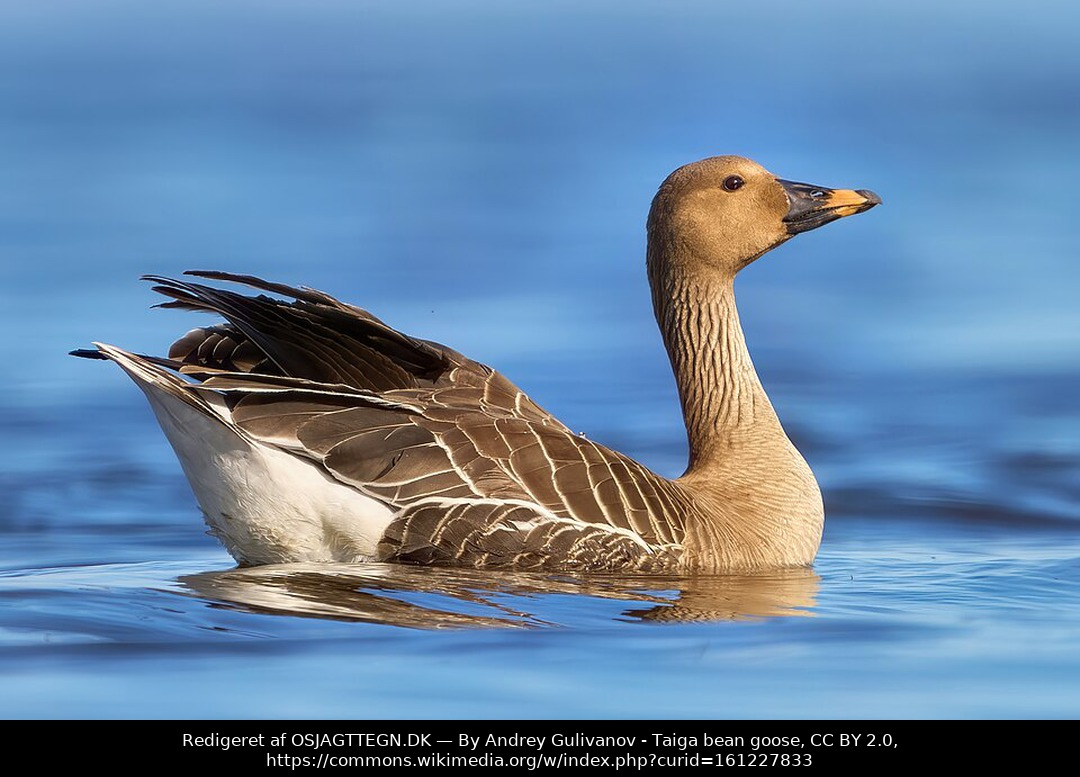
\includegraphics[width=\linewidth, height=7.2cm, keepaspectratio]{Billeder/Dyr/Fugle/Gaes/sædgås.jpg}
  \end{columns}
\end{frame}
% ========== BLISGÅS ==========
\begin{frame}{%
  \begin{minipage}[c]{0.30\textwidth}
    Blisgås
  \end{minipage}%
  \hfill
  \begin{minipage}[c]{0.45\textwidth}
    \footnotesize
    \textbf{Jagttid:} 1.\ september -- 31.\ januar
  \end{minipage}%
  \hfill
  \begin{minipage}[c]{0.15\textwidth}
    \noindent\raggedleft
    
\includegraphics[width=0.5cm, height=0.5cm, keepaspectratio]{Billeder/Ikoner/star.png}
  \end{minipage}%
}
  \vspace{0.25em}
  \begin{columns}[T]
    % --- Venstre kolonne: Tekst ---
    \column{0.45\textwidth}
    \setlength{\parskip}{0.5em}
    \tiny
    \RaggedRight
    \textbf{\textit{Anser albifrons}} – i familien "grå gæs" \par
    \textbf{Udseende:}\\
    \quad – Hvid blis ved næbroden, lyserødt næb, orange ben
    % --- Højre kolonne: Større billede ---
    \column{0.52\textwidth}
    \centering
    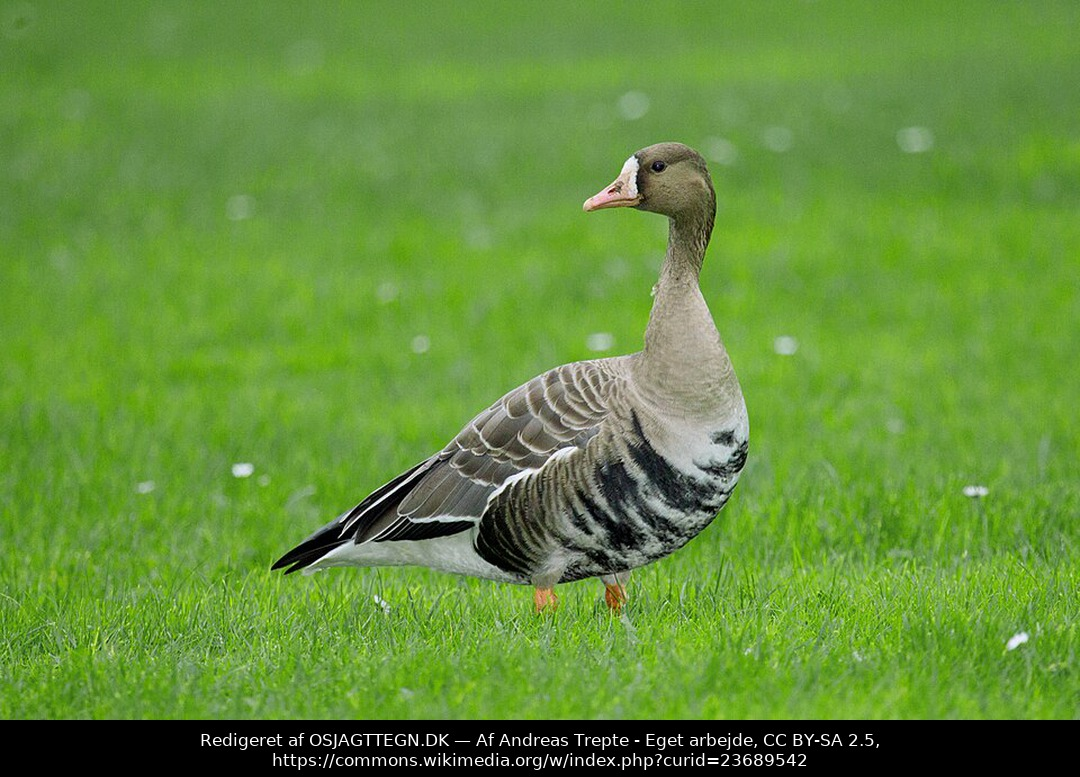
\includegraphics[width=\linewidth, height=7.2cm, keepaspectratio]{Billeder/Dyr/Fugle/Gaes/blisgås.jpg}
  \end{columns}
\end{frame}
% ========== BRAMGÅS ==========
\begin{frame}{%
  \begin{minipage}[c]{0.30\textwidth}
    Bramgås
  \end{minipage}%
  \hfill
  \begin{minipage}[c]{0.45\textwidth}
    \footnotesize
    \textbf{Jagttid:} Ingen jagttid
  \end{minipage}%
  \hfill
  \begin{minipage}[c]{0.15\textwidth}
    \noindent\raggedleft
    
\includegraphics[width=0.5cm, height=0.5cm, keepaspectratio]{Billeder/Ikoner/star.png}
  \end{minipage}%
}
  \vspace{0.25em}
  \begin{columns}[T]
    % --- Venstre kolonne: Tekst ---
    \column{0.45\textwidth}
    \setlength{\parskip}{0.5em}
    \tiny
    \RaggedRight
    \textbf{\textit{Branta leucopsis}} – lille rajgås som er i familie med knortegås og canadagås \par
    \textbf{Udseende:}\\
    \quad – Hvid kindplet der dækker det meste af hovedet
    % --- Højre kolonne: Større billede ---
    \column{0.52\textwidth}
    \centering
    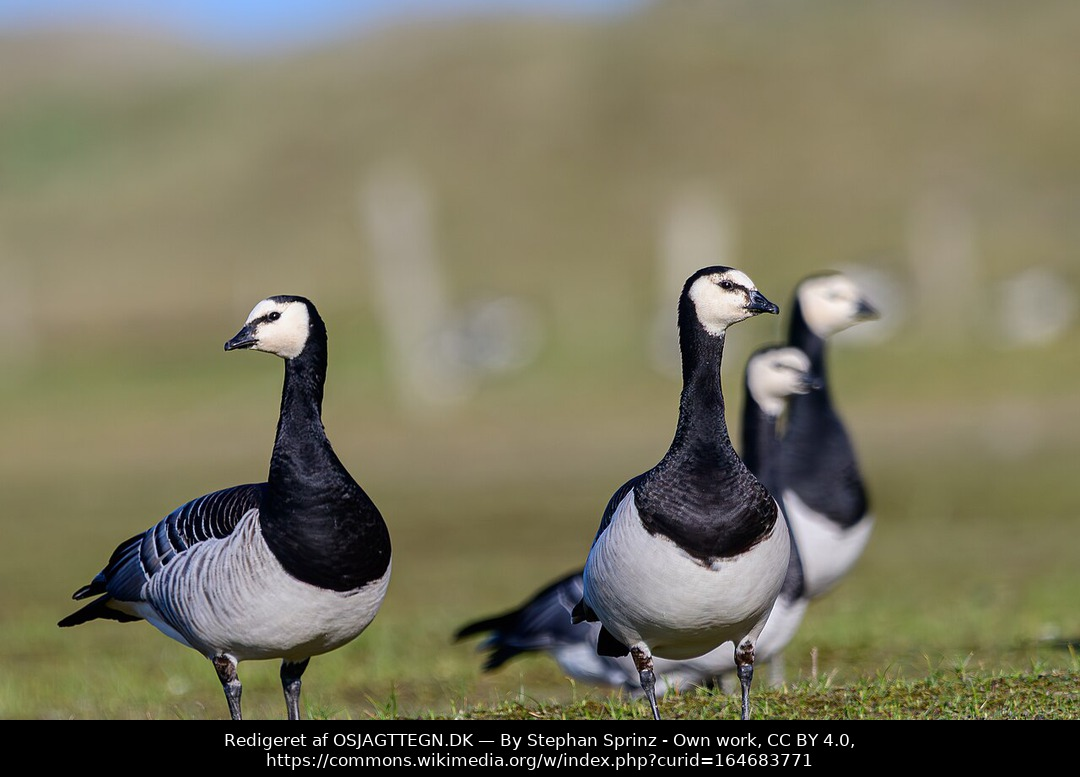
\includegraphics[width=\linewidth, height=7.2cm, keepaspectratio]{Billeder/Dyr/Fugle/Gaes/bramgås.jpg}
  \end{columns}
\end{frame}
% ========== CANADAGÅS ==========
\begin{frame}{%
  \begin{minipage}[c]{0.30\textwidth}
    Canadagås
  \end{minipage}%
  \hfill
  \begin{minipage}[c]{0.45\textwidth}
    \footnotesize
    \textbf{Jagttid:} 1.\ sep. -- 31.\ jan. samt 1.\ -- 31.\ aug.*
  \end{minipage}%
  \hfill
  \begin{minipage}[c]{0.15\textwidth}
    \noindent\raggedleft
    
\includegraphics[width=0.5cm, height=0.5cm, keepaspectratio]{Billeder/Ikoner/star.png}
  \end{minipage}%
}
  \vspace{0.25em}
  \begin{columns}[T]
    % --- Venstre kolonne: Tekst ---
    \column{0.45\textwidth}
    \setlength{\parskip}{0.5em}
    \tiny
    \RaggedRight
    \textbf{\textit{Branta canadensis}} – større hjemmehørende gås i rajgæs-familien \par
    \textbf{Udseende:}\\
    \quad – Stor krop og hvid plet bag øjet på kinden
    \par
    \textbf{* Jagttid 1. - 31. august:} \\
    \quad – \textbf{Krav} På arealer i omdrift (aktive marker/landbrug) med minimumsafstand på 300m til ferske vandre større end 3ha
    % --- Højre kolonne: Større billede ---
    \column{0.52\textwidth}
    \centering
    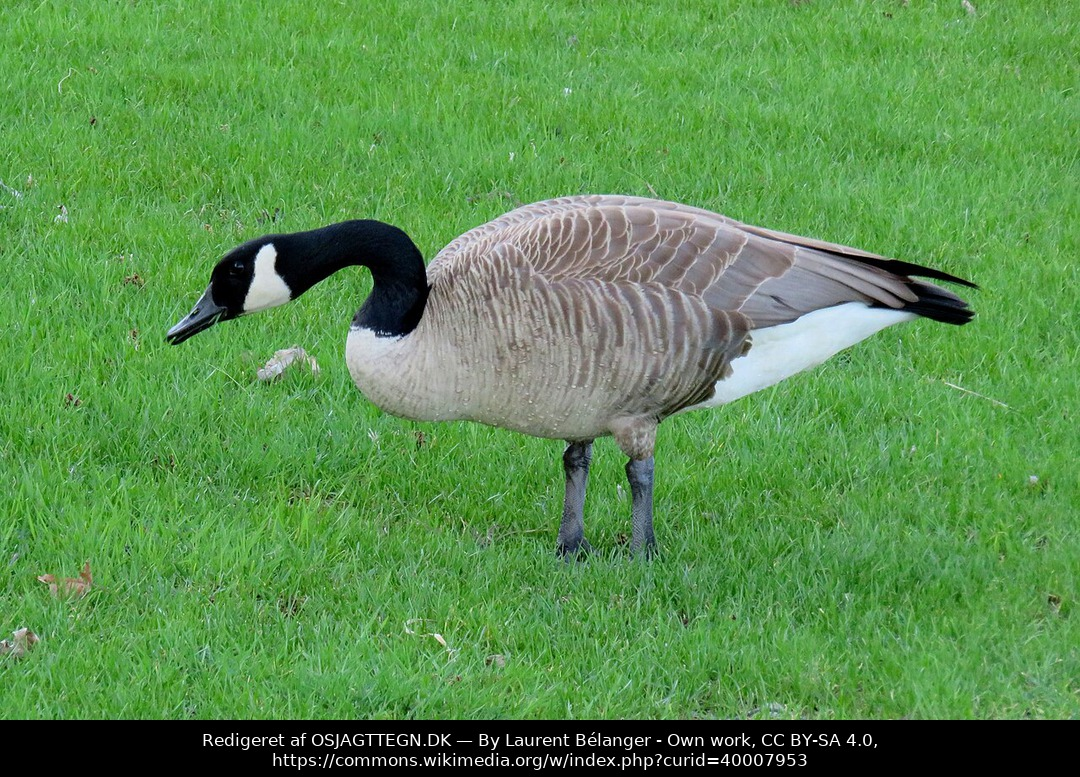
\includegraphics[width=\linewidth, height=7.2cm, keepaspectratio]{Billeder/Dyr/Fugle/Gaes/canadagås.jpg}
  \end{columns}
\end{frame}

\section{Storkefugle}

\begin{frame}
  \vspace{3em}
  \begin{center}
    {\LARGE \textbf{Storkefugle}}
    \vspace{2em}
    \\ Artsbestemmelse og vildtbiologi
\par
{\normalsize }
\vspace{1em}
\par
  \end{center}
\end{frame}

\begin{frame}{%
\begin{minipage}[t]{0.85\textwidth}
Fiskehejre
\end{minipage}%
\hfill
\begin{minipage}[t]{0.1\textwidth}
\raggedleft

\includegraphics[width=0.55cm, height=0.55cm, keepaspectratio]{Billeder/Ikoner/star.png}%
\end{minipage}%
}
\vspace{0.25em}
\begin{columns}[T]
% --- Venstre kolonne: Tekst ---
\column{0.55\textwidth}
\setlength{\parskip}{0.5em}
\small
\RaggedRight\textbf{\textit{Ardea cinerea}} – Særegen storkelignende slank fugl der jager langs kyster, søer, vandløb osv \par

\textbf{Udseende:} \\
\quad – Grå krop med sort nakketop, spidst langt gult næb \par

% --- Højre kolonne: Et billede ---
\column{0.40\textwidth}
\centering
\fbox{%
\begin{minipage}{\linewidth}
\centering
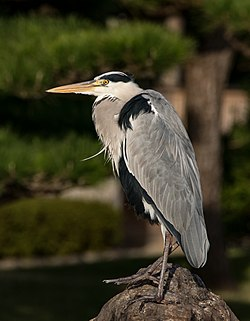
\includegraphics[width=0.8\linewidth, height=10cm, keepaspectratio]{Billeder/Dyr/Fugle/Hejrer/fiskehejre.jpg}
\end{minipage}
}%
\end{columns}
\end{frame}

\section{Årefodede fugle}

\begin{frame}
  \vspace{3em}
  \begin{center}
    {\LARGE \textbf{Årefodede fugle}}
    \vspace{2em}
    \\ Artsbestemmelse og vildtbiologi
\par
{\normalsize }
\vspace{1em}
\par
  \end{center}
\end{frame}

\begin{frame}{%
\begin{minipage}[t]{0.85\textwidth}
Skarv (mellemskarv og storskarv)
\end{minipage}%
\hfill
\begin{minipage}[t]{0.1\textwidth}
\raggedleft

\includegraphics[width=0.5cm, height=0.5cm, keepaspectratio]{Billeder/Ikoner/star.png}%
\hspace{0.2em}%

\includegraphics[width=0.5cm, height=0.5cm, keepaspectratio]{Billeder/Ikoner/star.png}
\end{minipage}%
}
\vspace{0.25em}
\begin{columns}[T]
% --- Venstre kolonne: Tekst ---
\column{0.55\textwidth}
\setlength{\parskip}{0.5em}
\small
\RaggedRight\textbf{\textit{Phalacrocorax carbo}} – Sort fugl også kaldet ålekrage \par % Rettet til Troldand's latinske navn og beskrivelse

\textbf{Udseende:} \\
\quad – Slank sort med kraftig gult næb der er tydeligt nedadbøjet i spidsen \par

\textbf{Levesteder:} \\
\quad – Kyster, fjorde, søer og større vandløb

\textbf{Føde:} \\
\quad – Fisk \par

\textbf{Udbredelse:} \\
\quad – Hele Danmark \par

\textbf{Træk/standfugl} \\
\quad – Mellemskarv yngler, storskarv er trækfugl \par

% --- Højre kolonne: Kun ét billede (Hannen) ---
\column{0.40\textwidth}
\centering
\fbox{%
\begin{minipage}{\linewidth}
\centering
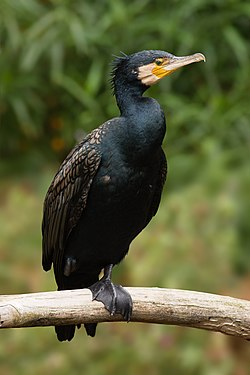
\includegraphics[width=0.8\linewidth, height=6.5cm, keepaspectratio]{Billeder/Dyr/Fugle/Skarver/skarv.jpg}%
\end{minipage}
}%
\end{columns}
\end{frame}

\section{Våbenhåndtering}

\begin{frame}
  \vspace{3em}
  \begin{center}
    {\LARGE \textbf{Våbenhåndtering}}
  \end{center}
\end{frame}



\begin{frame}{Våbenhåndtering – trin for trin}
  \vspace{0.3em} % Mindsket plads
  \begin{columns}[T]
    % --- Venstre kolonne: Opstart + Forhindring (Originalt indhold) ---
    \column{0.48\textwidth}
    \setlength{\parskip}{0.28em} % Mindsket afstand mellem afsnit
    \footnotesize
    \RaggedRight

    \textbf{-- Opstart --} \\
    1. Fødder i skudretning – fri for mennesker. \\
    2. Forskæfte med \textit{modsatte hånd} af skulderen du vil lægge geværet til. \\
    3. Åbn geværet lodret med topnøgle. \\
    4. Kig igennem – \textit{tomt og rent}. \\
    5. Før gennem vandret (knækket). \\
    6. Isæt patroner. \\
    7. Luk i \textbf{45°} – hør \textit{klik}. \\
    8. Før op til \textit{semi-klar}. \\
    9. \textit{Fingre væk} fra aftrækker/sikring. \par

    \vspace{0.3em} % Mindsket plads
    \textbf{-- Forhindring --} \\
    10. Før geværet ned gennem vandret. \\
    11. Åbn – patroner \textit{i lommen}. \\
    12. Forcer med \textit{knækket gevær}. \\
    13. Efterse løbene. \\
    14. Isæt patroner igen. \\
    15. Før op gennem vandret. \par

    % --- Højre kolonne: Skudafgivelse (Originalt indhold) ---
    \column{0.48\textwidth}
    \setlength{\parskip}{0.28em} % Mindsket afstand mellem afsnit
    \footnotesize
    \RaggedRight

    \textbf{-- Skudafgivelse --} \\
    16. Geværet lades \\
    17. Op til \textit{semi-klar}. \\
    18. Kolbe mod bryst – nær armhule. Min 30° \\
    19. Meld: \textbf{„KLAR!“} \\
    20. Afsikring \textit{frem}. \\
    21. Affyr 1–2 skud. \\
    22. Ned til bryst. \\
    23. Sikring \textit{tilbage}. \\
    24. Ned gennem vandret. \\
    25. Åbn – fjern afskudte. \\
    26. Gentag \textbf{4 gange}. \\
    27. Aflever \textit{alle patroner}. \par

  \end{columns}
\end{frame}

\section{Jagt fra kunstige skjul}

\begin{frame}
  \vspace{3em}
  \begin{center}
    {\LARGE \textbf{Jagt fra kunstige skjul}
    }
    \\
    \vspace{1em}
    Bekendtgørelse om udsætning af vildt, jagtmåder og jagtredskaber
    \\
    \vspace{1em}
    BEK nr 1652 af 19/12/2017, Kapitel 1
  \end{center}
\end{frame}

\begin{frame}
    \frametitle{Forbud mod jagt på pattedyr fra kunstige skjul (§ 1)}

    \vspace{1.5cm}

    § 1

    \vspace{0.5cm}

    Der må ikke drives jagt på pattedyr fra

    \vspace{0.5cm}

    1) kunstigt skjul, herunder hus, hytte, jordhul, eller

    \vspace{0.5cm}

    2) platform eller sæde, der er hævet mere end 50 cm over det omgivende terræn.

    \vspace{0.5cm}

    Med to undtagelser

    \vspace{2.5cm}
\end{frame}

\begin{frame}
    \frametitle{Varianter af kunstige skjul}

    \begin{columns}
        \column{0.5\textwidth}
        \centering
        \begin{figure}
            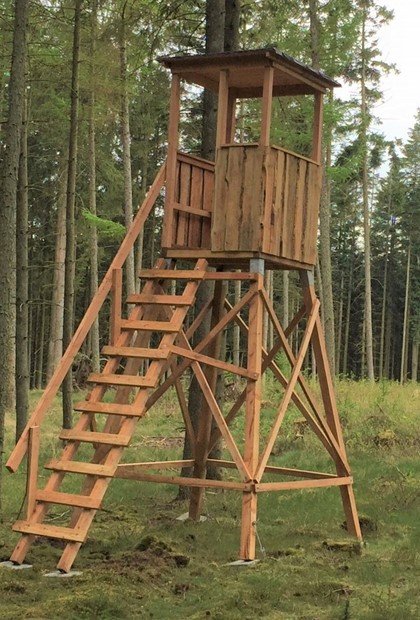
\includegraphics[width=0.5\textwidth]{Billeder/Redskaber/jagttårn.jpg}
            \caption{\textbf{Jagttårn} (jægeren kan skyde stående)}
        \end{figure}
        
        \column{0.5\textwidth}
        \centering
        \begin{figure}
            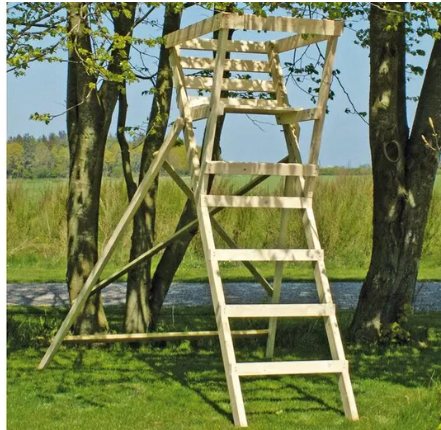
\includegraphics[width=0.5\textwidth]{Billeder/Redskaber/jagtstige.png}
            \caption{\textbf{Jagtstige} (jægeren kan skyde siddende)}
        \end{figure}
    \end{columns}

    \vspace{1cm}  % Plads til tekst under

    \centering
\end{frame}

\begin{frame}
    \frametitle{Regler for skydetårne (§ 1)}

    \begin{columns}[T]  % T for top-alignment
        \column{0.6\textwidth}
        \begin{itemize}
            \item Højere end 50 cm over omkringliggende areal
            \item Min 130 m til skel med mindre andet er aftalt skriftligt
            \item Udført i træ eller metal
            \item Opsættes i min 0,5 hektar skov eller ydre/inde skovbryn
            \item Må ikke skæmme (samme højde som øvrig bevoksning)
            \item Højde til plateau max 5m
            \item Sider max 110cm høje
            \item Plateau max 2 $m^2$
            \item Tag i et plan, ikke-reflekterende, max 10 cm udhæng
        \end{itemize}
        
        \column{0.4\textwidth}
        \centering
        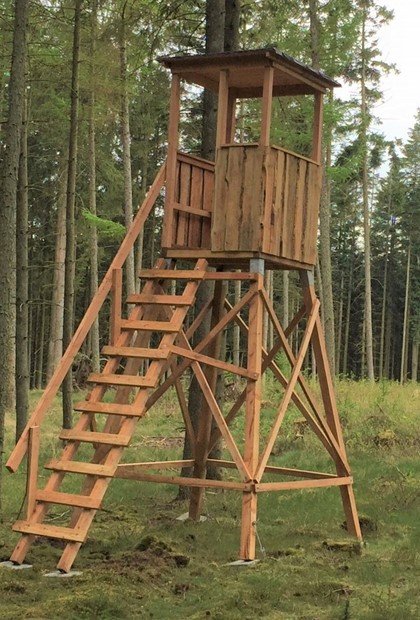
\includegraphics[width=0.7\textwidth]{Billeder/Redskaber/jagttårn.jpg}  % Mindre billede nu
        \vspace{0.5cm}
        \small 
    \end{columns}

\end{frame}

\begin{frame}
    \frametitle{Regler for skydestiger (§ 1)}

    \begin{columns}[T]  % T for top-alignment
        \column{0.6\textwidth}
        \begin{itemize}
            \item Højere end 50 cm over omkringliggende areal
            \item Min 130 m til skel med mindre andet er aftalt skriftligt
            \item De skal være mobile eller midlertidige konstruktioner
            \item Opsættes i hegn eller bevoksninger (ikke 0,5 hektar regel)
            \item Må ikke skæmme (samme højde som øvrig bevoksning)
            \item Højde til plateau max 5 m
        \end{itemize}
        
        \column{0.4\textwidth}
        \centering
        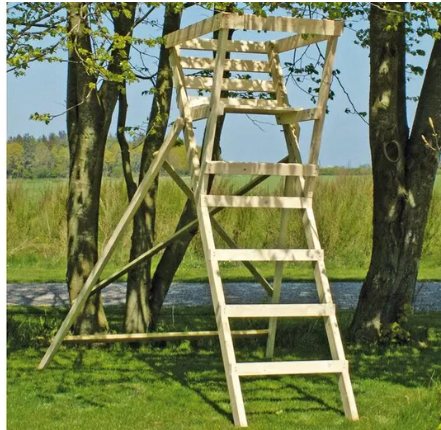
\includegraphics[width=0.7\textwidth]{Billeder/Redskaber/jagtstige.png}  % Mindre billede nu
        \vspace{0.5cm}
        \small 
    \end{columns}

    \end{frame}

\begin{frame}
    \frametitle{Regler for kunstige skjul på fugle (§ 3)}

    \begin{columns}[T]  % T for top-alignment
        \column{0.6\textwidth}
        \begin{itemize}
            \item Gulvet/ståstedet må højest være hævet 50 cm over terrænnet
            \item Ellers er kreativiteten ubegrænset – brug camouflage, net, siv, grene osv.
            \item Skjulet kan være midlertidigt (flytbart) eller mere fast (f.eks. ramme med net)
            \item Ofte brugt til andejagt, duejagt eller kragejagt med lokkefugle
            \item Husk at våbentype skal passe til skjulet (typisk haglgevær til fugle) (§ 2)
            \item Skjulet skal camouflages godt for ikke at skræmme vildtet
        \end{itemize}
        
        \column{0.4\textwidth}
        \centering
        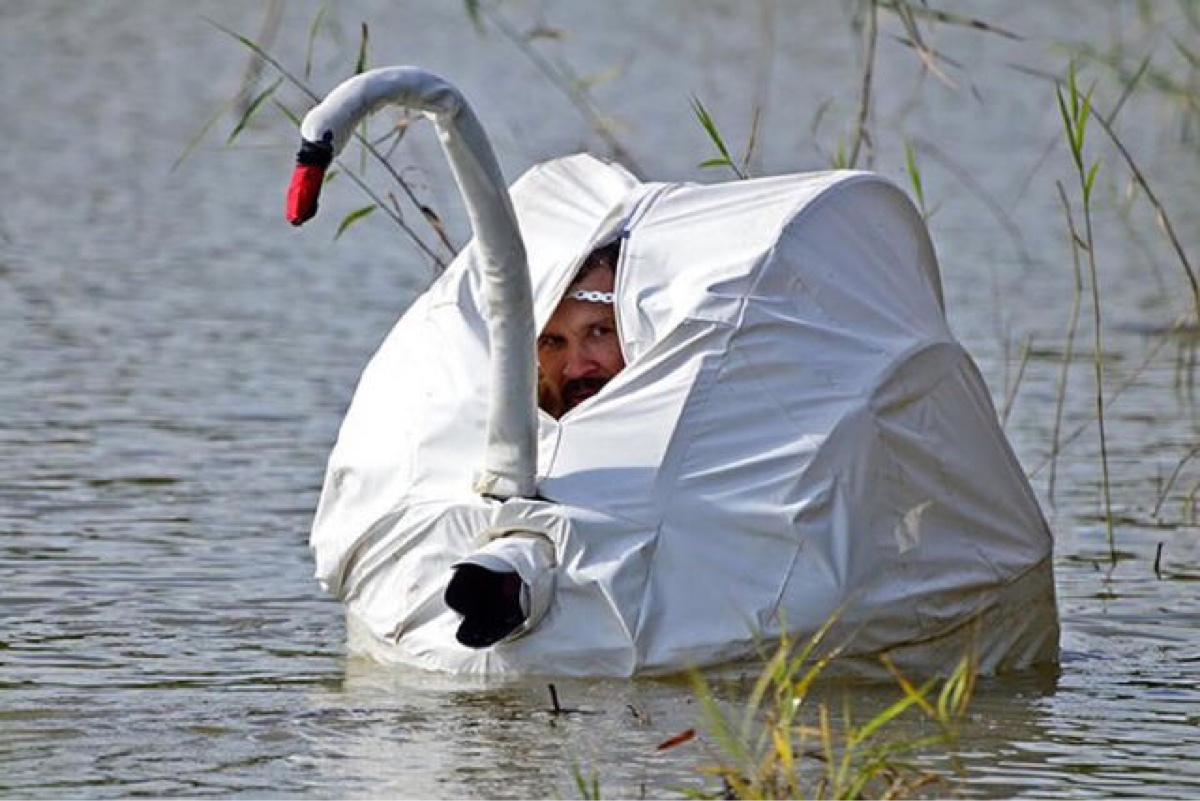
\includegraphics[width=0.9\textwidth]{Billeder/Redskaber/kunstigtskjul.jpg}
        \vspace{0.5cm}
        
    \end{columns}

\end{frame}


\section{Jagttermer - Del 1}

\begin{frame}
  \vspace{3em}
  \begin{center}
    {\LARGE \textbf{Jagttermer - Del 1}
    }
    \\
    \vspace{1em}
  \end{center}
\end{frame}


\begin{frame}{Jagttermer - Del 1 (A-F)}

\vspace{0.3em} % Mindre top-afstand

\begin{columns}[T]
    % --- Venstre kolonne: A-C ---
    \column{0.48\textwidth}
    \textbf{\large A, B, C}
    \setlength{\parskip}{0.1em} % Mindre afstand mellem punkter
    \scriptsize % Mindre skriftstørrelse
    \RaggedRight
    \begin{itemize}
        \item \textbf{Anskudssted:} Stedet, hvor vildtet blev ramt.
        \item \textbf{Anskyde:} Ramme vildt uden at skuddet er dræbende.
        \item \textbf{Afskydning:} Mængden af vildt skudt på et terræn.
        \item \textbf{Apport:} Kommando til hund om at hente nedlagt vildt.
        \item \textbf{Anstandsjagt:} Ventejagt fra et udvalgt sted.
        \item \textbf{Bagskud:} Skud til vildt, der løber/flyver direkte væk.
        \item \textbf{Bladet:} Primært træfområde på hårvildt (hjerte/lunger).
        \item \textbf{Brunsttid:} Tidsrummet, hvor parring foregår.
        \item \textbf{Brække op:} Åbne klovbærende vildt og tage indvoldene ud.
    \end{itemize}

    % --- Højre kolonne: D-F ---
    \column{0.48\textwidth}
    \textbf{\large D, E, F}
    \setlength{\parskip}{0.1em} % Mindre afstand mellem punkter
    \scriptsize % Mindre skriftstørrelse
    \RaggedRight
    \begin{itemize}
        \item \textbf{Doublé:} Nedlægge to stykker vildt i to skud i træk.
        \item \textbf{Esser:} Fødesøgning for hjortevildt og hare.
        \item \textbf{Fald:} 1) Ekskrementer 2) Stor ankomst af trækfugle.
        \item \textbf{Fangstskud:} Skud, der aflives anskudt vildt med.
        \item \textbf{Forende:} Dø (om vildt).
        \item \textbf{Forlægge:} Partere vildt (især klovbærende).
        \item \textbf{Fouragere:} Vildtets fødesøgning (andet end hjortevildt/hare).
        \item \textbf{Fællesjagt:} Organiseret jagt med et større antal deltagere.
    \end{itemize}
\end{columns}

\end{frame}

\end{document}